\chapter{Building a Baseline for Quantitiative Risk Assessments}


\begin{center}\vspace{-0.5\baselineskip}\parbox{0.85\textwidth}{\small\itshape
We conducted a\index{risk assessment} \gls{riskassessment} to better understand the \gls{threat}\index{threat} of criminal action against an in-house system.  We examined both \index{cybercrime}\gls{cybercrime} and physical crimes using data that was normalized to a\index{per capita} \gls{percapita} rates of crimes.  We drew from \gls{fbi} \gls{ic3} annual reports and\index{Chattanooga} Chattanooga Police\index{open data} Open Data records.  The \index{population}\gls{population}\index{sample} \gls{sample}s were taken from the\index{US Census} \gls{us} Census Bureau reports.  We were able to build a baseline simulation that can be used to better understand the context of the likelihood and severity of observed events in the lab.\par}\end{center}
\section{Introduction}
\begin{figure}[H]
  \centering
  \rotatebox{0}{\scalebox{1}{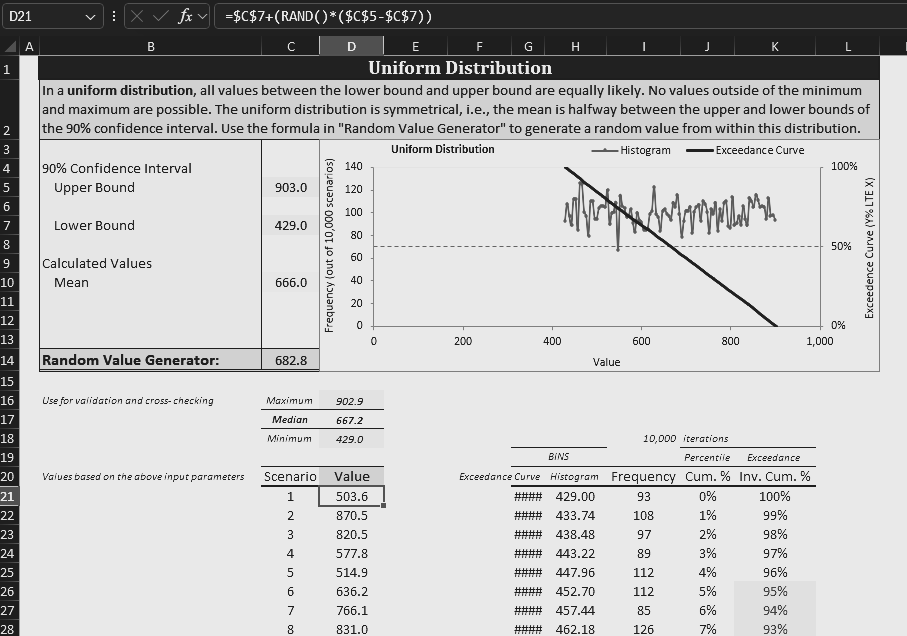
\includegraphics[width=\linewidth]{figures/Screenshot 2026-07-28 145652.png}}}
  \caption{Example run of a\index{Monte Carlo simulation} \gls{montecarlo} using state-level data to set bounds.  Here we chose\index{personal data breach} Personal \gls{databreach} victim counts from 2016 and 2022 as upper and lower bounds. 10,000 rows projected randomized values between these bounds and determined\index{mean} \gls{mean} and counts by\index{confidence interval} \gls{confidenceinterval}.
  \protect\endnote{Monte Carlo Modeling Toolkit authored by Derek E. Brink, \gls{cissp}, \url{www.linkedin.com/in/derekbrink}. March 2023.}
  }
  \label{fig:screenshot-montecarlo1}
\end{figure}
\subsection{Background and Content}
We had a modest amount of education in\index{statistics} \gls{statistics} as we began the project.  Our skills were derived primarily from three college courses.  At\index{Chattanooga}\index{Chattanooga State Community College} Chattanooga State Community College in 2011, we had courses in "Elementary Statistics." \endnote{Triola, Mario F. Elementary Statistics Technology Update + Mystatlab Student Access Code Card. Pearson College Division, 2012.} This was an algebra-based course that focused on the fundamentals of applying data to\index{normal distribution} \gls{normaldistribution}s.  Also there in 2012, we had a course in "Statistics for Engineers." \endnote{Levine, David M, et al. Applied Statistics for Engineers and Scientists. Pearson, 2001.} This was an algebra-based course that discussed various quality control techniques and\index{statistical} statistical modeling.  In 2023 at\index{Harvard University Extension School} Harvard University Extension School, we had a graduate course in "Risk in Information Security" with Derek Brink.  \endnote{Hubbard, Douglas W, and Richard Seiersen. How to Measure Anything in Cybersecurity Risk. Wiley, 2016.}  Professor Brink authored the Excel spreadsheet which we have used for\index{Monte Carlo simulation} \gls{montecarlo}s.

\begin{figure}[H]
  \centering
  \rotatebox{0}{\scalebox{1}{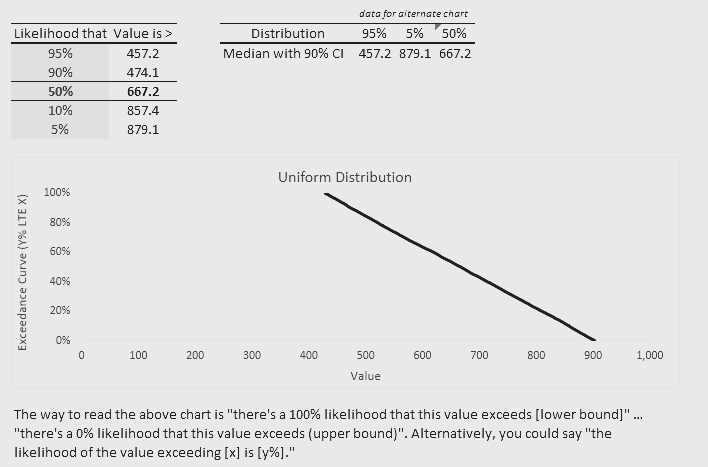
\includegraphics[width=\linewidth]{figures/Screenshot 2026-07-28 145609.png}}}
  \caption{Example results of applying\index{Monte Carlo simulation} \gls{montecarlo} to forecasting.  Here we see the assertion that there is a 90\% likelihood that the number of victims will be between 457 and 879; the\index{mean} \gls{mean} of the simulation was 667.\protect\endnote{Monte Carlo Modeling Toolkit authored by Derek E. Brink, CISSP, \url{www.linkedin.com/in/derekbrink}. March 2023.}}
  \label{fig:screenshot-montecarlo2}
\end{figure}

The spreadsheet conducts 10,000 simulations of data points between user-supplied bounds.  Sheets in the Excel workbook are capable of conducting a variety of these simulations.  They are differentiated by modeling style (uniform, triangular,\index{normal distribution} normal, \gls{binary}, or\index{discrete} discrete) and points of interest (count, cost, or percentage).

Each of the simulating rows follows these general steps:
\begin{itemize}
\item{Reference the lower bound.}
\item{Ascertain the range between lower and upper bounds.}
\item{Generate a random number.}
\item{Multiply the random number against the range value.}
\item{Install the generated random value in a cell.}
\end{itemize}
The row values are then counted, sorted, and ranked into\index{confidence interval} \gls{confidenceinterval}s.  The values and critical points are plotted on various graphs.  The end result is that it is easy for an opertor of the spreadsheet to generate a\index{Monte Carlo simulation} \gls{montecarlo} of a\index{distribution} \gls{distribution} between bounds.  Since there are enough iterations (10,000), the simulation can have\index{statistical} statistical value.  Since the inputs on the spreadsheet can be readily modified and since the cells are calculated upon page saving or loading, new simulations can be run with ease.  We recognized Professor Brink's spreadsheet was a useful tool that we could apply to forecasts of interest to us here.
\subsection{Problem Statement}
We need a cheap source of risk information to inform procedural decisions in the lab.  We can't afford to pay a vendor for intelligence feeds.  Free \gls{attack}-specific feeds that work well for defense technologies like Snort or Suricata are not in a form that would inform policy-level risk decisions.  We want to gather this information efficiently and without generating any civil or criminal liability or threats; we're not going to conduct firsthand research in \index{cybercrime} \gls{cybercrime} forums to determine what shape a localized risk might take.  We want to be able to  use publicly available \index{cybercrime} \gls{cybercrime} data in order to persue commercial-grade decisions on a localized scale in a manner that is informed and practical.

These conditions suggest that we should use the following resources:
\begin{itemize}
  \item \gls{us} \gls{ic3} data
  \item \gls{cert} data from other nations
  \item\index{open data} Open Data from local government agencies
  \item MITRE ATT\&CK for guiding data selection
  \item Other scientifically valid\index{open data} Open Data sources.
\end{itemize}

We found during our research that there would sometimes be promising documents published by security vendors and software companies.  Unfortunately, many of those were not accompanied by scientifically valid\index{open data} open data sources.  So it is with caution that we could sometimes accept the assertions; however, we sometimes found that the reports were useless beyond identifying an anecdotal cause, condition, or effect.  Without data to quantify those identified conditions, we were sometimes left with a good idea that could not be proven in a manner that supported a\index{risk assessment!quantitative} quantitative \gls{riskassessment}.  In those times, those leads had to sometimes be abandoned or be allowed to fall short of their potential impact.  Unscientific assertions from vendors seemed to be a trend in our research environment; unscientific assertions from vendors is such a part of the problem's environment that it is a problem almost unto itself.

\subsection{Project Objectives}
We want to be able to conduct a quantative \gls{riskassessment} for our small project lab that would be scientific and illustrative enough to allow others to accept it as guidance.

We want others to be able to conduct their own\index{risk assessment} risk assessments
and be able to use these notes as a pattern for their own benefit.

We want to be able to use scaled-to-size \gls{ic3} data in a\index{Monte Carlo simulation} \gls{montecarlo} as a baseline for understanding the potential rates and severity of \gls{cybercrime} encounters.

We want to proceed with an educated, professionally supported philosophical framework of ideas.  We didn't want to decay into philosophical edge cases like harshly questioning cause and effect, blindly ignoring unquantified threats, or emotionally fueling conspiratorial fears.  We need to keep our feet on the ground and our systems defended; but, if the\index{risk assessment} \gls{riskassessment} shows that threats are rare or severe, then we need to understand that through quantitative analysis.

\subsubsection{Limits on\index{hypothesis testing} \Gls{hypothesis} Testing}
By themselves, the\index{Monte Carlo simulation} \gls{montecarlo}s will allow us to make some narrow assertions, but for the\index{statistics} \gls{statistics} to have greater local benefit follow-on data gathering and analysis would be needed.  In this project we are scaling down national and state level data to a more localized scope.  However, that doesn't provide us with testable\index{hypothesis} \gls{hypothesis}.  These\index{statistics} statistics could be used as a baseline for understanding the context of other treatments, measurements, or forecasts; but, by themselves, there will be little we can prove or disprove with our simulations.  We will be able to make simple assertions about the likelihood and severity of impact certain \gls{cybercrime} types may have on our\index{sample} \gls{sample}, but we will not be able to forecast the effectiveness of any local treatments, mitigations, or defensive techniques.

\subsection{Scope of Work}
We chose to limit our risk analysis to the algebraic scaling of \gls{ic3} data on Excel spreadsheets to limit the calculations by hand.  The data has four main trends (victim count, victim impact, suspect count, suspect impact), but to keep the analysis productive we would proceed all the way through with victim count.  This would support an assessment of likelihood.  Then we would go through the mathematics again to determine severity by scaling the values of victim impact.  With those two categories available, we would have the minimum amount of data needed to conduct a quantitative assessment of likelihood and severity.  This would meet the minimum expectations of most\index{risk assessment} risk assessments' data analysis needs.

We would need to scope the data to understand it in a verifiable context.  Since our goal is to analyze a project-sized scaling, we would need to couch that target between verifiable guideposts.  So, we chose to scale state-level data to our city's \index{population}\gls{population}.  Alongside this, we could scale state-level data to a small organization's size (e.g. 150 people as stakeholders).  Since that scaled data would be calculated, we would want to present it in context with states and territories that represented high and low levels of \index{cybercrime} \gls{cybercrime} (California and \index{American Samoa} American Samoa).  This way we would set a scope that would allow a reader to see the effect of scaling from known states down to the small business organization level.
\subsection{Variables}
Not all of the collected \gls{ic3} data categories were stable over time.  As the reports were produced year to year, new threats emerged and the \index{cybercrime} \gls{cybercrime} field changed.  This meant that some categories that were present at the older end of our analysis (2016) were not present at the end of our sampling (2022) or later.  Because of this, we had to ignore some categories or combine others.  Variability in criminal activity affected reporting.

This had indirect effects on our analysis.  Check Fraud and Credit Card Fraud, as activity titles, changed over the years.  Threats to people, in the form of both Terrorism and Stalking, changed over the years.  This meant that we chose to ignore some categories that would seem to have value to commercial businesses while combining counts into one category in others.  Our picking and choosing among the categories genuinely shapes the risk picture we're considering as we do the\index{risk assessment} \gls{riskassessment}.  Our projects and labs can't live in a fictional world where entire \gls{threat} categories don't exist; but, we had to keep the data calculatable in order to proceed.

\subsection{Assumptions, Risks, and Limitations}
We set out to better understand the rates of computer-related crimes in our area using public data sources.  We drew from \gls{fbi} \gls{ic3} annual reports and\index{Chattanooga} Chattanooga Police\index{open data} open data records.  The \gls{ic3} reports provided categorical breakdowns of different types of internet-related crimes.  In the past, we were able to find per-state breakdowns of those crimes.  The \gls{fbi} would provide four views of computer crime:  overall count, overall financial impact, victim count, and per-victim financial impact.  This was available both nationally and per state.  When following up in 2026, we noticed we were only able to immediately discover the national-level summaries of crime.

Anecdotally, we know that we have witnessed several of these crimes at rates higher than shown in these tables (Tables \ref{tab:chattanoogacrime2}, \ref{tab:chattanoogacrime3}, \ref{tab:chattanoogacrime4}).  We suspect that we're seeing numbers this low because few victims are taking the steps necessary to report computer crimes to federal authorities.  For example, when companies or individuals encounter \gls{ransomware}\index{ransomware}, their reactions may involve repairing the afffected endpoint but not informing law enforcement.  Nonetheless, those authorities have been the public's observable source of crime reporting.  While we continue to use this data, we may need to accept that true counts of \index{cybercrime}\gls{cybercrime} in the city must be scaled by an unknown factor.

The\index{Chattanooga}\index{Chattanooga!Police Department} Chattanooga Police Department, like other departments of the City of\index{Chattanooga} Chattanooga, participate in an\index{open data} open data project.  Anonymonized crime reports are provided to the public in a manner that lets us track by approximate region of the city and by category of crime.  We chose to do this because we recognized some crimes would be reported to local police that were not reported to federal authorities.  Some crimes, such as physical break-ins, were more likely to be handled by local police.  Since the systems involved are in-scope for physical damage, we felt the\index{Chattanooga}\index{Chattanooga!Police Department} Chattanooga Police Department's\index{open data} open data would be the best public source for supporting criminal \gls{threat} forecasts for events like burglary from a vehicle.  Some of the crime categories, such as extortion or threats against a person, could be reported to either federal \gls{ic3} or local police; the nature of the threats might be different; but, there may be more direct physical threats reported to local police; there is no formal mimetic analysis that would shuttle a threatening complaint to one law enforcement agency or another.  Meanwhile, some locally policed crimes may focus upon:  employees, facility safeguards, loss of computer equipment in public, loss of computer equipment by theft from facilities or vehicles, and so on.

As we examine the data from the public data sources and we feel that the reported rates are less than our experience would justify, we have to recognize that there may be shortcomings in the reported data.  Perhaps we would do well to scale the rates up to meet our experience.  However, those arbitrary inflations would damage the validity of our academic risk calculations.  So, for the time being, we leave the inflation or deflation of the end results for the reader as a localized adjustment.  Since our main goal is to show a method for determining the risks through the reported data, it could be argued that the exact numbers are less relevant than the demonstrated methods.
\subsubsection{Limitations Imposed by Federal Law Enforcement in Tennessee}
During our research, one shocking fact came to light.  At the Cybersecurity Summit conference in Nashville, TN in 2023, Derek Rousseau, a Special Agent from the \gls{fbi} Nashville Cyber Squad, presented and answered a Q\&A.  To our surprise, the special agent answered a direct question, How much money needs to be at stake for the \gls{fbi} to get involved in a \index{cybercrime} \gls{cybercrime}?  His answer was that the \gls{us} Attorney in Nashville wanted to see at least \$100,000 in damage for domestic crimes or \$400,000 in damage for international crimes.  For damage amounts below that, it was not effective to devote an \gls{fbi} special agent to investigate the crime.  As a result, the special agent encouraged the reporting of smaller crimes so that cases could be aggregated against a suspect to levels that merited federal investigation and prosecution.  Later, as we compare \gls{ic3} crime data, we'll see that many of the annual totals are below these limits.  This suggests that the \gls{us} is prosecuting only a fraction of those reported crimes that affect the \index{population}\gls{population}.
\subsubsection{Limitations Derived from Reporting}
Another limitation on our projections arises from the voluntary nature of the reporting.  Since victims or defenders need to advise the \gls{ic3} of a security event, only those who follow through with the voluntary reporting actions will get counted.  Commercial defenders will see that in their experience only a small number of daily cybersecurity events will seem worthy to report to federal law enforcement; the scope of true attacks would seem through those anecdotes to be much greater than the reported numbers.  Since all of the reports are likely to be initiated by those who speak up, we cannot escape the experimental design problems associated with a\index{sample!convenience}\index{convenience sample} convenience \gls{sample} when using \gls{ic3} data for our\index{statistics} \gls{statistics}.

As we've seen and will see, the grouping of those reports does not match our experimental needs.  States and nations are simply too large to be of practical benefit to defenders.  Most small businesses and organizations will need the value of public information; commercial vendors can provide similar data for a fee; we need the free data, but we need to tailor it down to the size of a defending organization to apply it realistically to\index{risk assessment} risk assessments for cybersecurity defense.
\subsection{Significance of the Project}
We hope to take the mystery out of public\index{statistics} \gls{statistics} for cybersecurity use.  We want to provide the types of workshop examples we've seen locally in\index{open data} open data workshops \endnote{"City of Chattanooga Hub." Chattanooga.Gov, 2025, \url{https://data.chattanooga.gov/}. Accessed 4 Aug. 2026.} but in technical note form.  Ideally, readers should be able to follow these notes and then craft their own projects for forecasting cybersecurity risk using publicly available data sources.
\section{Literature Review}
\subsection{Overview of Existing Solutions or Approaches}
\subsection{Comparisons of Technologies or Frameworks}
\subsection{Gaps in the Literature}
We haven't found many examples outside of college classrooms that allow readers to follow the extrapolation process and formulate their own forecasts for cybersecurity risks.  While there are excellent books on the topics of\index{statistics} \gls{statistics} and cybersecurity, we havent' found works that took public data like this and used it for other purposes.

In our hometown of\index{Chattanooga} Chattanooga, there have been public non-profit efforts to use\index{open data} open data in workshops that are free and open to the public.  Most of the data sets used for those activities are part of local government's participation in an\index{open data} open data initiative. \endnote{"City of Chattanooga Hub." Chattanooga.Gov, 2025, \url{https://data.chattanooga.gov/}} By working through Jupyter notebooks and group discussions, participants might learn more about public bicycle rental use, for example.  Our interests, meanwhile, lay firmly within the cybersecurity realm.
\section{Methodology}
\begin{figure}[H]
  \centering
  \rotatebox{0}{\scalebox{1}{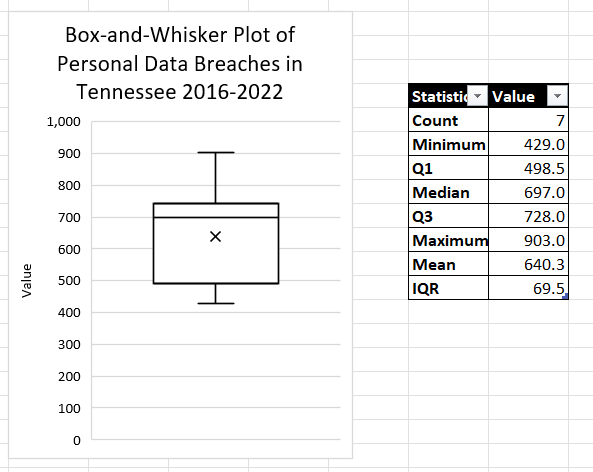
\includegraphics[width=\linewidth]{figures/boxwhisker-tnpersdatabreach2016.png}}}
  \caption{Seven year summary of\index{personal data breach} Personal Data Breaches in Tennessee reported to \gls{ic3}. }
  \label{fig:screenshot-boxwhisker-tnpersdatabreach2016}
\end{figure}
We took \index{cybercrime} \gls{cybercrime} data from a seven year span of \gls{ic3} publications.  The annual reports for the nation and for each state showed a count of victims per category of \index{cybercrime} \gls{cybercrime}.  The \gls{us} \gls{fbi} defined each category for their report.  We put that data into a\index{matrix} \gls{matrix}, organized by year and category of crime.

Each state we chose got its own\index{matrix} \gls{matrix}. We noticed that three states typically had high counts of crime; they were: \index{California} California,\index{Texas} Texas, and\index{Florida} Florida.  We noticed that \gls{us} territories, like \index{American Samoa} American Samoa, \gls{us} Virgin Islands, and\index{Puerto Rico} Puerto Rico, were reported also as if they were a state.  These smaller areas with lower \index{population}\gls{population}s also showed lowed low counts of \index{cybercrime} \gls{cybercrime}.  We chose these high crime areas (e.g.\index{California} California) and low crime areas (e.g. \index{American Samoa} American Samoa) as our guides for choosing maximum and minimum limits.  Our desired target areas were chosen by the target's home state; our intial runs included \index{Chattanooga} Chattanooga, Tennessee.

\subsection{Using State Data to Forecast a Company's Data}

Our main data sets are provided in the public interest; they're based on large units of people like states and nations.  As system operators, we have a much smaller interest; we're interested in company sized elements.  Instead of being concerned with the \index{cybercrime} \gls{cybercrime} fate of over 300 million Americans or 9 million Tennesseans, we are probably more interested in what might happen to 100 stakeholders.

To smooth out the counts of \index{cybercrime} \gls{cybercrime} into rates, we adjusted these state victim counts \index{per capita}\gls{percapita}.  We chose the\index{US Census} \gls{us} Census reports for those years to be the \index{population}\gls{population} values of the states.  This would provide us with a\index{per capita} \gls{percapita} rate of \index{cybercrime} \gls{cybercrime} based on the chosen state which represented the chosen limit or target in the \index{distribution}\gls{distribution}.

Formally, we note this process below as shown in Figure \ref{fig:statcalc-percap}.  $R$ represents our result.  $N_t$ represents our constant for target \index{sample}\gls{sample} \index{population}\gls{population} and is used for multiplying the rate to \index{scale}scale it to match the \index{population}\gls{population} of the target. $t$ represents our starting year for the \index{sample}\gls{sample} from \gls{ic3} and coordinates the rows until it progresses to the final year chosen which is denoted by $n$. $i$ represents our chosen category \index{index}index of \index{cybercrime} \gls{cybercrime}. $j$ represents our year index and is built with $t$ until it progresses to the final year of the \index{sample}\gls{sample} denoted by $n$. $P_j$ represents the \index{population}\gls{population} of the target city at year $j$, drawn from \index{matrix}\gls{matrix} $P$.

\begin{figure}[H]
  \centering




\[
R_j = N_t \sum_{j=t}^{t+6} \frac{X_{j,i}}{P_j}, \quad \text{where } X_{j,i} = \begin{cases} M_{j,i} & \text{if victim count} \\ V_{j,i} & \text{if victim impact} \\ S_{j,i} & \text{if suspect count} \\ D_{j,i} & \text{if suspect impact} \end{cases}
\]

  \caption{Notation for the\index{statistical} statistical calculation of the security event\index{matrix} \gls{matrix} adjusted for\index{per capita} \gls{percapita} rates of incidence.}
  \label{fig:statcalc-percap}
\end{figure}

Five\index{matrix} matrices inform this calculation.  The first, $P$ as shown in Figure \ref{fig:statcalc-popmatrix}, records the target city \index{population}\gls{population} for each year of the \index{sample}\gls{sample} as a single column.

\begin{figure}[H]
  \centering

\[
P=
\text{Years }\left\{
\begin{matrix}
t\\ \vdots\\ j\\ \vdots\\ n
\end{matrix}
\right.
\left[
\begin{array}{c}
\multicolumn{1}{c}{%
  \overbrace{\hphantom{p_{t}}}^{\text{Population}}%
}\\
p_t \\
\vdots \\
p_j \\
\vdots \\
p_n
\end{array}
\right]
\]

  \caption{Structure of the \index{sample}\gls{sample} \index{population}\gls{population}\index{matrix} \gls{matrix} indexed by year.}
  \label{fig:statcalc-popmatrix}
\end{figure}

The second\index{matrix} \gls{matrix}, $M$ as shown in Figure \ref{fig:statevent-victimcount}, organises the raw \index{cybercrime} \gls{cybercrime} counts from \gls{ic3} by category and year, where each entry $a_{j,i}$ is a count that will be adjusted to a\index{per capita} \gls{percapita} rate.


\begin{figure}[H]
  \centering
\[
M=
\text{Years }\left\{
\begin{matrix}
t\\ \vdots\\ j\\ \vdots\\ n
\end{matrix}
\right.
\left[
\begin{array}{ccccccc}
\multicolumn{7}{c}{%
  \overbrace{%
    \hphantom{a_{t,1}\ \cdots\ a_{t,2}\ \cdots\ a_{t,i}\ \cdots\ a_{t,m}}%
  }^{\text{Victim Counts by Categories}}%
}\\
a_{t,1} & \cdots & a_{t,2} & \cdots & a_{t,i} & \cdots & a_{t,m} \\
\vdots  & \ddots & \vdots  & \ddots & \vdots  & \ddots & \vdots \\
a_{j,1} & \cdots & a_{j,2} & \cdots & a_{j,i} & \cdots & a_{j,m} \\
\vdots  & \ddots & \vdots  & \ddots & \vdots  & \ddots & \vdots \\
a_{n,1} & \cdots & a_{n,2} & \cdots & a_{n,i} & \cdots & a_{n,m}
\end{array}
\right]
\]

  \caption{Structure of the security event\index{matrix} \gls{matrix} for victim counts by \index{cybercrime} \gls{cybercrime} categories indexed by year.}
  \label{fig:statevent-victimcount}
\end{figure}


The third\index{matrix} \gls{matrix}, $V$ as shown in Figure \ref{fig:statevent-victimimpact}, organises the victim impact in USD from \gls{ic3} by category and year, where each entry $a_{j,i}$ is a count that will be adjusted later to a\index{per capita} \gls{percapita} rate.
\begin{figure}[H]
  \centering
\[
V=
\text{Years }\left\{
\begin{matrix}
t\\ \vdots\\ j\\ \vdots\\ n
\end{matrix}
\right.
\left[
\begin{array}{ccccccc}
\multicolumn{7}{c}{%
  \overbrace{%
    \hphantom{a_{t,1}\ \cdots\ a_{t,2}\ \cdots\ a_{t,i}\ \cdots\ a_{t,m}}%
  }^{\text{Victim Impacts by Categories}}%
}\\
a_{t,1} & \cdots & a_{t,2} & \cdots & a_{t,i} & \cdots & a_{t,m} \\
\vdots  & \ddots & \vdots  & \ddots & \vdots  & \ddots & \vdots \\
a_{j,1} & \cdots & a_{j,2} & \cdots & a_{j,i} & \cdots & a_{j,m} \\
\vdots  & \ddots & \vdots  & \ddots & \vdots  & \ddots & \vdots \\
a_{n,1} & \cdots & a_{n,2} & \cdots & a_{n,i} & \cdots & a_{n,m}
\end{array}
\right]
\]


  \caption{Structure of the security event\index{matrix} \gls{matrix} for victim impacts, as in dollars of damage, by \index{cybercrime} \gls{cybercrime} categories indexed by year.}
  \label{fig:statevent-victimimpact}
\end{figure}

The fourth\index{matrix} \gls{matrix}, $S$ as shown in Figure \ref{fig:statevent-suspectcount}, organises the count of suspects from \gls{ic3} by category and year.  Each entry $a_{j,i}$ helps us to understand how many suspects are operating within an area of concern.  This is a count that will be adjusted later to a\index{per capita} \gls{percapita} rate.

\begin{figure}[H]
  \centering
\[
S=
\text{Years }\left\{
\begin{matrix}
t\\ \vdots\\ j\\ \vdots\\ n
\end{matrix}
\right.
\left[
\begin{array}{ccccccc}
\multicolumn{7}{c}{%
  \overbrace{%
    \hphantom{a_{t,1}\ \cdots\ a_{t,2}\ \cdots\ a_{t,i}\ \cdots\ a_{t,m}}%
  }^{\text{Suspect Counts by Categories}}%
}\\
a_{t,1} & \cdots & a_{t,2} & \cdots & a_{t,i} & \cdots & a_{t,m} \\
\vdots  & \ddots & \vdots  & \ddots & \vdots  & \ddots & \vdots \\
a_{j,1} & \cdots & a_{j,2} & \cdots & a_{j,i} & \cdots & a_{j,m} \\
\vdots  & \ddots & \vdots  & \ddots & \vdots  & \ddots & \vdots \\
a_{n,1} & \cdots & a_{n,2} & \cdots & a_{n,i} & \cdots & a_{n,m}
\end{array}
\right]
\]

  \caption{Structure of the security event\index{matrix} \gls{matrix} for suspect counts by \index{cybercrime} \gls{cybercrime} categories indexed by year.  These counts consider the number of actors who engage victims in a given area.}
  \label{fig:statevent-suspectcount}
\end{figure}

The fifth\index{matrix} \gls{matrix}, $D$ as shown in Figure \ref{fig:statevent-suspectdamage}, organises the damages attributed by suspects in USD from \gls{ic3} by category and year, where each entry $a_{j,i}$ is a count that will be adjusted later to a\index{per capita} \gls{percapita} rate.  This helps us to understand rates of effective impact, per suspect, in a given area.

\begin{figure}[H]
  \centering
\[
D=
\text{Years }\left\{
\begin{matrix}
t\\ \vdots\\ j\\ \vdots\\ n
\end{matrix}
\right.
\left[
\begin{array}{ccccccc}
\multicolumn{7}{c}{%
  \overbrace{%
    \hphantom{a_{t,1}\ \cdots\ a_{t,2}\ \cdots\ a_{t,i}\ \cdots\ a_{t,m}}%
  }^{\text{Suspect Damage by Categories}}%
}\\
a_{t,1} & \cdots & a_{t,2} & \cdots & a_{t,i} & \cdots & a_{t,m} \\
\vdots  & \ddots & \vdots  & \ddots & \vdots  & \ddots & \vdots \\
a_{j,1} & \cdots & a_{j,2} & \cdots & a_{j,i} & \cdots & a_{j,m} \\
\vdots  & \ddots & \vdots  & \ddots & \vdots  & \ddots & \vdots \\
a_{n,1} & \cdots & a_{n,2} & \cdots & a_{n,i} & \cdots & a_{n,m}
\end{array}
\right]
\]

  \caption{Structure of the security event\index{matrix} \gls{matrix} for suspect damage, in dollars by perpetrators, by \index{cybercrime} \gls{cybercrime} categories indexed by year.  This tally helps us understand how damaging each actor is to victims.}
  \label{fig:statevent-suspectdamage}
\end{figure}


We apply these\index{matrix} matrices to the formula shown in Figure \ref{fig:statcalc-percap}. The entries $a_{j,i}$ are the raw counts taken from the \gls{ic3} state-level reports for the chosen source state.  Dividing each entry by $P_j$ converts it to a\index{per capita} \gls{percapita} rate; multiplying by $N_t$ then scales that rate to match the \index{population}\gls{population} of the target city.  The \index{population}\gls{population} values in $P$ provide the year-by-year context for $N_t$ and confirm the representativeness of the scaling.  Summing the selected column $i$ of the\index{per capita} \gls{percapita}-adjusted $M$ across all years yields the final result $R$.
\subsection{Methodology for\index{Monte Carlo simulation} \Gls{montecarlo}s in Excel}
We chose \gls{ic3} crime data from \index{American Samoa} American Samoa to act as our lower bound.  We chose data from California to act as our upper bound.  We set those limits by looking at seven year spans of crime data and taking the\index{median} \gls{median}.  This means we would be likely to have observations above and below the limits, but that the limits themselves would have a basis in observation.
We input and processed the data as follows:
\begin{itemize}
\item We imported the data from \gls{ic3} crime tables
\item We calculated counts and costs for:
  \begin{itemize}
    \item \index{Chattanooga} Chattanooga
    \item \index{American Samoa} American Samoa
    \item \index{California} California.
  \end{itemize}
\item We imported a\index{normal distribution} \gls{normaldistribution} table from the\index{Monte Carlo simulation} \gls{montecarlo} Toolkit.
\item We set\index{mean} \gls{mean} summary counts from\index{American Samoa} American Samoa as our lower bound.
\item We set\index{mean} \gls{mean} summary counts from\index{California} California as our upper bound.
\item We accepted the\index{Monte Carlo simulation} \gls{montecarlo} percentages and exceedence curves.
\end{itemize}

There were times when it was obvious that a\index{normal distribution} \gls{normaldistribution} would not fit.  When there was a choice between a count of 0 and 1 events, we ran a supplementary \gls{binary}\index{distribution} \gls{distribution}.  When there was a choice of less than 8 events, we ran a supplementary\index{discrete} discrete\index{distribution} \gls{distribution}.  We needed to change the\index{distribution} \gls{distribution} type when modeling the count or likelihood of an event; we did not need to change from a\index{normal distribution} \gls{normaldistribution} when modeling impact because the range of currency was not overly narrow.

%%%%%%%%%%%%%%%%%%%%%%% POPULATION %%%%%%%%%%%%%%%%%%%%%%%
\subsection{\Gls{population} Changes During\index{sample} Sampled Years}
\begin{table}[H]
  \centering
  \caption{Changes to \index{population}\Gls{population} in Key Areas}
  \label{tab:chattanoogacrime1}
  \begin{tabular}{@{}>{\centering\arraybackslash}
  p{0.10\linewidth} >{\centering\arraybackslash}
  p{0.07\linewidth} >{\centering\arraybackslash}
  p{0.07\linewidth} >{\centering\arraybackslash}
  p{0.07\linewidth} >{\centering\arraybackslash}
  p{0.07\linewidth} >{\centering\arraybackslash}
  p{0.07\linewidth} >{\centering\arraybackslash}
  p{0.07\linewidth} >{\centering\arraybackslash}
  p{0.09\linewidth} >{\centering\arraybackslash}
  p{0.07\linewidth}}
    \toprule
    \textbf{Year} &
    \rotatebox{90}{\begin{tabular}{@{}ll@{}}\index{American Samoa} American Samoa\\Population\end{tabular}} &
    \rotatebox{90}{\begin{tabular}{@{}ll@{}}References\end{tabular}} &
    \rotatebox{90}{\begin{tabular}{@{}ll@{}}City of \index{Chattanooga} Chattanooga\\Population\end{tabular}} &
    \rotatebox{90}{\begin{tabular}{@{}ll@{}}References\end{tabular}} &
    \rotatebox{90}{\begin{tabular}{@{}ll@{}}State of Tennessee\\Population\end{tabular}} &
    \rotatebox{90}{\begin{tabular}{@{}ll@{}}References\end{tabular}} &
    \rotatebox{90}{\begin{tabular}{@{}ll@{}}State of\index{California} California\\Population\end{tabular}} &
    \rotatebox{90}{\begin{tabular}{@{}ll@{}}References\end{tabular}}

    \\
    \midrule
2016&52,245&\endnote{\url{https://fred.stlouisfed.org/series/POPTOTASA647NWDB}}&177,746&\endnote{\url{https://www.census.gov/quickfacts/chattanoogacitytennessee}}&6,646,010&\endnote{\url{https://www.census.gov/quickfacts/fact/table/TN/PST045222}}&39,149,186&\endnote{\url{https://fred.stlouisfed.org/series/CAPOP}}\\
2017&51,586&\endnote{\url{https://fred.stlouisfed.org/series/POPTOTASA647NWDB}}&179,530&\endnote{\url{https://www.census.gov/quickfacts/chattanoogacitytennessee}}&6,708,799&\endnote{\url{https://www.census.gov/quickfacts/fact/table/TN/PST045222}}&39,337,785&\endnote{\url{https://fred.stlouisfed.org/series/CAPOP}}\\
2018&50,908&\endnote{\url{https://fred.stlouisfed.org/series/POPTOTASA647NWDB}}&181,918&\endnote{\url{https://www.census.gov/quickfacts/chattanoogacitytennessee}}&6,771,631&\endnote{\url{https://www.census.gov/quickfacts/fact/table/TN/PST045222}}&39,437,463&\endnote{\url{https://fred.stlouisfed.org/series/CAPOP}}\\
2019&50,209&\endnote{\url{https://fred.stlouisfed.org/series/POPTOTASA647NWDB}}&182,799&\endnote{\url{https://www.census.gov/quickfacts/chattanoogacitytennessee}}&6,829,174&\endnote{\url{https://www.census.gov/quickfacts/fact/table/TN/PST045222}}&39,437,610&\endnote{\url{https://fred.stlouisfed.org/series/CAPOP}}\\
2020&49,751&\endnote{\url{https://fred.stlouisfed.org/series/POPTOTASA647NWDB}}&181,560&\endnote{\url{https://www.census.gov/quickfacts/chattanoogacitytennessee}}&6,925,619&\endnote{\url{https://www2.census.gov/programs-surveys/popest/datasets/2020-2022/state/totals/NST-EST2022-POPCHG2020_2022.csv}}&39,538,223&\endnote{\url{https://fred.stlouisfed.org/series/CAPOP}}\\
2021&49,225&\endnote{\url{https://fred.stlouisfed.org/series/POPTOTASA647NWDB}}&181,163&\endnote{\url{https://www.census.gov/quickfacts/chattanoogacitytennessee}}&6,968,351&\endnote{\url{https://www2.census.gov/programs-surveys/popest/datasets/2020-2022/state/totals/NST-EST2022-POPCHG2020_2022.csv}}&39,152,927&\endnote{\url{https://fred.stlouisfed.org/series/CAPOP}}\\
2022&48,342&\endnote{\url{https://fred.stlouisfed.org/series/POPTOTASA647NWDB}}&184,086&\endnote{\url{https://www.census.gov/quickfacts/chattanoogacitytennessee}}&7,051,339&\endnote{\url{https://www2.census.gov/programs-surveys/popest/datasets/2020-2022/state/totals/NST-EST2022-POPCHG2020_2022.csv}}&39,125,347&\endnote{\url{https://fred.stlouisfed.org/series/CAPOP}}\\

    \bottomrule \end{tabular}
\raggedright{City \index{population}\gls{population} based on the\index{US Census} \gls{us} Census reported \index{population}\gls{population} for the City of\index{Chattanooga} Chattanooga itself.  Surrounding satellite cities and unincorporated areas within the Hamilton County, Tennessee, were not included. \index{population}\Gls{population} for the State of Tennessee provided perspective on calculated rates in later tables. \index{population}\Gls{population} for \index{American Samoa} American Samoa and the State of\index{California} California were included for perspective on maximum and minimum counts in later tables.}
\end{table}


\subsection{Corporate and Personal Data Breaches}

\begin{table}[H]
  \centering
  \caption{Projected In-City Victim Counts, City of\index{Chattanooga} Chattanooga, Threats to System Intrusion}
  \label{tab:chattanoogacrime2}
  \begin{tabular}{@{}>{\centering\arraybackslash}
  p{0.05\linewidth} >{\centering\arraybackslash}
  p{0.35\linewidth} >{\centering\arraybackslash}
  p{0.35\linewidth} >{\centering\arraybackslash}
  p{0.05\linewidth}}
    \toprule
    Year
    &Data Breach
    &Personal Data Breach
    &\\
    \midrule


2016&1&11&\endnote{original\protect\url{https://www.ic3.gov/Media/PDF/AnnualReport/2016State/StateReport.aspx\#?s=47} current \protect\url{https://www.ic3.gov/AnnualReport/Reports/2016_IC3Report.pdf}}\\
2017&1&13&\endnote{original:\protect\url{https://www.ic3.gov/Media/PDF/AnnualReport/2017State/StateReport.aspx\#?s=47} current: \url{https://www.ic3.gov/AnnualReport/Reports/2017_IC3Report.pdf}}\\
2018&0&18&\endnote{original:\protect\url{https://www.ic3.gov/Media/PDF/AnnualReport/2018State/StateReport.aspx\#?s=47} current: \url{https://www.ic3.gov/AnnualReport/Reports/2018_IC3Report.pdf}}\\
2019&0&13&\endnote{original:\protect\url{https://www.ic3.gov/Media/PDF/AnnualReport/2019State/StateReport.aspx\#?s=47} current: \url{https://www.ic3.gov/AnnualReport/Reports/2019_IC3Report.pdf}}\\
2020&0&18&\endnote{original:\protect\url{https://www.ic3.gov/Media/PDF/AnnualReport/2020State/StateReport.aspx\#?s=47} current: \url{https://www.ic3.gov/AnnualReport/Reports/2020_IC3Report.pdf}}\\
2021&0&19&\endnote{original:\protect\url{https://www.ic3.gov/Media/PDF/AnnualReport/2021State/StateReport.aspx\#?s=47} current: \url{https://www.ic3.gov/AnnualReport/Reports/2021_IC3Report.pdf}}\\
2022&1&23&\endnote{original:\protect\url{https://www.ic3.gov/Media/PDF/AnnualReport/2022State/StateReport.aspx\#?s=47} current: \url{https://www.ic3.gov/AnnualReport/Reports/2022_IC3Report.pdf}}\\

    \bottomrule \end{tabular}
  \raggedright{Counts deduced from \gls{ic3} Victim Complaints for Tennessee adjusted for a per-capita rate and then multiplied by the city's \index{population} population for that year.}
\end{table}

%%%%%%%%%%%%%%%%%%%%  DATA BREACH %%%%%%%%%%%%%%%%%%%%%%%%
\newpage
\subsection{Data Breach}
\subsubsection{Lower Bound Computation}
\[
\begin{bmatrix}
\mathbf{x}_{\text{American Samoa}}^{(\text{count})}\\
\mathbf{x}_{\text{American Samoa}}^{(\text{dollars})}
\end{bmatrix}
=
\begin{bmatrix}
0 & \cdots & 0 & \cdots & 0\\
\$0 & \cdots & \$0 & \cdots & \$0
\end{bmatrix}.
\]
% Columns represent years 2016, \cdots, 2017, \cdots, 2022 for American Samoa Data Breach.
% Raw counts: 2016=0, 2017=0, 2022=0.  Raw dollars: 2016=\$0, 2017=\$0, 2022=\$0.
\[
\begin{bmatrix}
\mathbf{x}_{\text{American Samoa}}^{(\text{count scaled to sample population})}\\
\mathbf{x}_{\text{American Samoa}}^{(\text{dollars scaled to sample population})}
\end{bmatrix}
=
\begin{bmatrix}
0 & \cdots & 0 & \cdots & 0\\
\$0 & \cdots & \$0 & \cdots & \$0
\end{bmatrix}.
\]
% Per-capita scaled to Chattanooga population: 2016=0, 2017=0, 2022=0 victims; dollars: all \$0.
  \[
\bar{X}_{\text{American Samoa}}^{(m)}
= \frac{1}{N}\sum_{i=1}^{N} X_{\text{American Samoa},i}^{(m)},
\]
\\
\[
\qquad
m \in \{\text{scaled count},\text{scaled dollars}\}
\]
\[
\begin{bmatrix}
\bar{X}_{\text{American Samoa}}^{(\text{scaled count})}\\
\bar{X}_{\text{American Samoa}}^{(\text{scaled dollars})}
\end{bmatrix}
=
\begin{bmatrix}
0.43\\
\$166{,}890
\end{bmatrix}.
\]
\subsubsection{Upper Bound Computation}
\[
\begin{bmatrix}
\mathbf{x}_{\text{California}}^{(\text{count})}\\
\mathbf{x}_{\text{California}}^{(\text{dollars})}
\end{bmatrix}
=
\begin{bmatrix}
568 & \cdots & 632 & \cdots & 381\\
\$9{,}769{,}361 & \cdots & \$7{,}805{,}797 & \cdots & \$1
\end{bmatrix}.
\]
% Columns represent years 2016, \cdots, 2017, \cdots, 2022 for California Data Breach.
\[
\begin{bmatrix}
\mathbf{x}_{\text{California}}^{(\text{count scaled to sample population})}\\
\mathbf{x}_{\text{California}}^{(\text{dollars scaled to sample population})}
\end{bmatrix}
=
\begin{bmatrix}
2 & \cdots & 2 & \cdots & 2\\
\$34{,}399 & \cdots & \$24{,}702 & \cdots & \$121{,}084
\end{bmatrix}.
\]
\[
\bar{X}_{\text{California}}^{(m)}
= \frac{1}{N}\sum_{i=1}^{N} X_{\text{California},i}^{(m)},
\]
\\
\[
\qquad
m \in \{\text{scaled count},\text{scaled dollars}\}
\]
\[
\begin{bmatrix}
\bar{X}_{\text{California}}^{(\text{scaled count})}\\
\bar{X}_{\text{California}}^{(\text{scaled dollars})}
\end{bmatrix}
=
\begin{bmatrix}
1.26\\
\$44{,}615
\end{bmatrix}.
\]
\subsubsection{Monte Carlo Simulations for Likelihood and Impact}
\begin{figure}[H]
  \centering
  \rotatebox{0}{\scalebox{1}{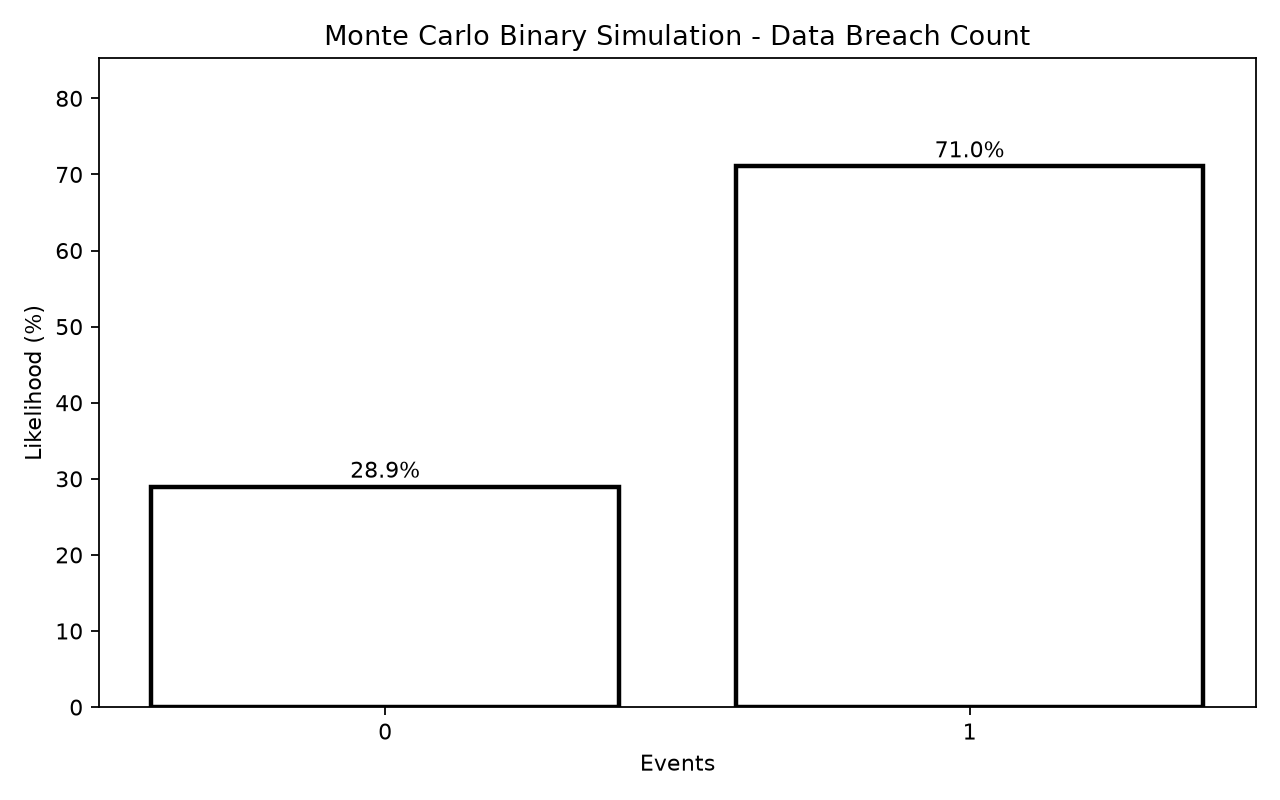
\includegraphics[width=\linewidth]{figures/binary_dataBreach_count.png}}}
  \caption{We ran a\index{Monte Carlo simulation} Monte Carlo simulation of 10,000 iterations with a \gls{binary} distribution to spread random instances between upper and lower bounds taken from the means of seven year samples. We bounded between 0 and 1 possible \index{data breach}\gls{databreach} events over a year.\protect\endnote{\index{sample} Sample size was set equivalent to the City of\index{Chattanooga} Chattanooga to determine the per capita rates for each year over data from \index{American Samoa} American Samoa and\index{California} California.  The means of those rates were used to set upper and lower bounds with \index{American Samoa} American Samoa and\index{California} California representing low and high \index{cybercrime} \gls{cybercrime} counts respectively.}
  \protect\endnote{Monte Carlo Modeling Toolkit authored by Derek E. Brink, \gls{cissp}, \url{www.linkedin.com/in/derekbrink}. March 2023.}
  }
  \label{fig:screenshot-montecarlo-\gls{databreach}-count-binary}
\end{figure}
When we computed the upper and lower bounds, we recognized that a normal distribution would not fit well for forecasting likelihood.  We took the mean of the sample from American Samoa for the lower bound (0); we took the mean from the sample from California for the upper bound (1); we had a separation of 1 unit.  Therefore, we switched to a \gls{binary} model with 2 possible outcomes.
\begin{table}[H]
  \centering
  \caption{Monte Carlo \gls{binary} Simulation Values for \gls{databreach}}
  \label{tab:binary_databreach_montecarlo}
  \begin{center}
  \begin{tabular}{@{}>{\centering\arraybackslash}
  p{0.30\linewidth} >{\centering\arraybackslash}
  p{0.20\linewidth} >{\centering\arraybackslash}
  p{0.20\linewidth}}
    \toprule
Events
&0
&1\\
    \midrule
Likelihood
&29.0\%
&71.0\%\\
    \bottomrule \end{tabular}
    \end{center}
  \raggedright{A\index{Monte Carlo simulation} Monte Carlo simulation was run using a \gls{binary} distribution.  We bounded the simulation between 0 and 1 events.  The probability of a \index{data breach}\gls{databreach} occurring was set to 71\% based on the midpoint of the American Samoa lower bound (0.43) and the California upper bound (1.0).  The resulting distribution showed the effect of randomness on each possible outcome.}
\end{table}

\begin{figure}[H]
  \centering
  \rotatebox{0}{\scalebox{1}{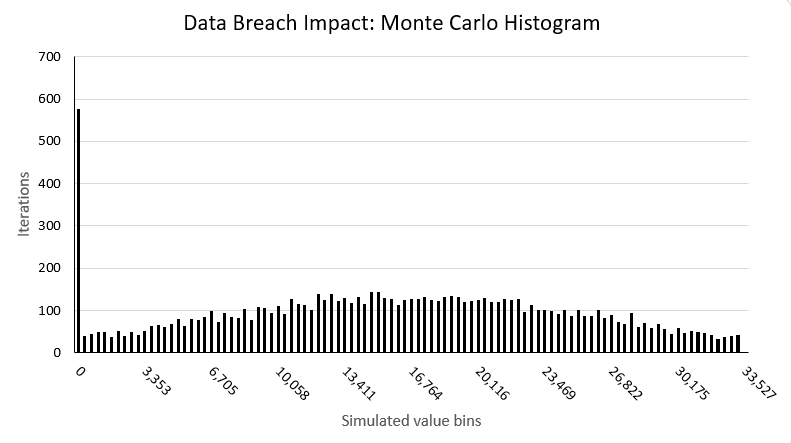
\includegraphics[width=\linewidth]{figures/histogram_dataBreach_impact.png}}}
  \caption{We ran a\index{Monte Carlo simulation} Monte Carlo simulation of 10,000 iterations with a normal distribution to spread random instances between bounds taken from means of seven year samples. We set a lower bound that the events would cost at \$0.  We set an upper bound that the events would cost \$33{,}527.27.  \protect\endnote{\index{sample} Sample size was set equivalent to the City of\index{Chattanooga} Chattanooga to determine the per capita rates for each year over data from \index{American Samoa} American Samoa and\index{California} California.  The means of those rates were used to set upper and lower bounds with \index{American Samoa} American Samoa and\index{California} California representing low and high \index{cybercrime} \gls{cybercrime} impact values respectively.}
  \protect\endnote{Monte Carlo Modeling Toolkit authored by Derek E. Brink, \gls{cissp}, \url{www.linkedin.com/in/derekbrink}. March 2023.}
  }
  \label{fig:screenshot-montecarlo-databreach\index{databreach}-impact-histo}
\end{figure}
\begin{figure}[H]
  \centering
  \rotatebox{0}{\scalebox{1}{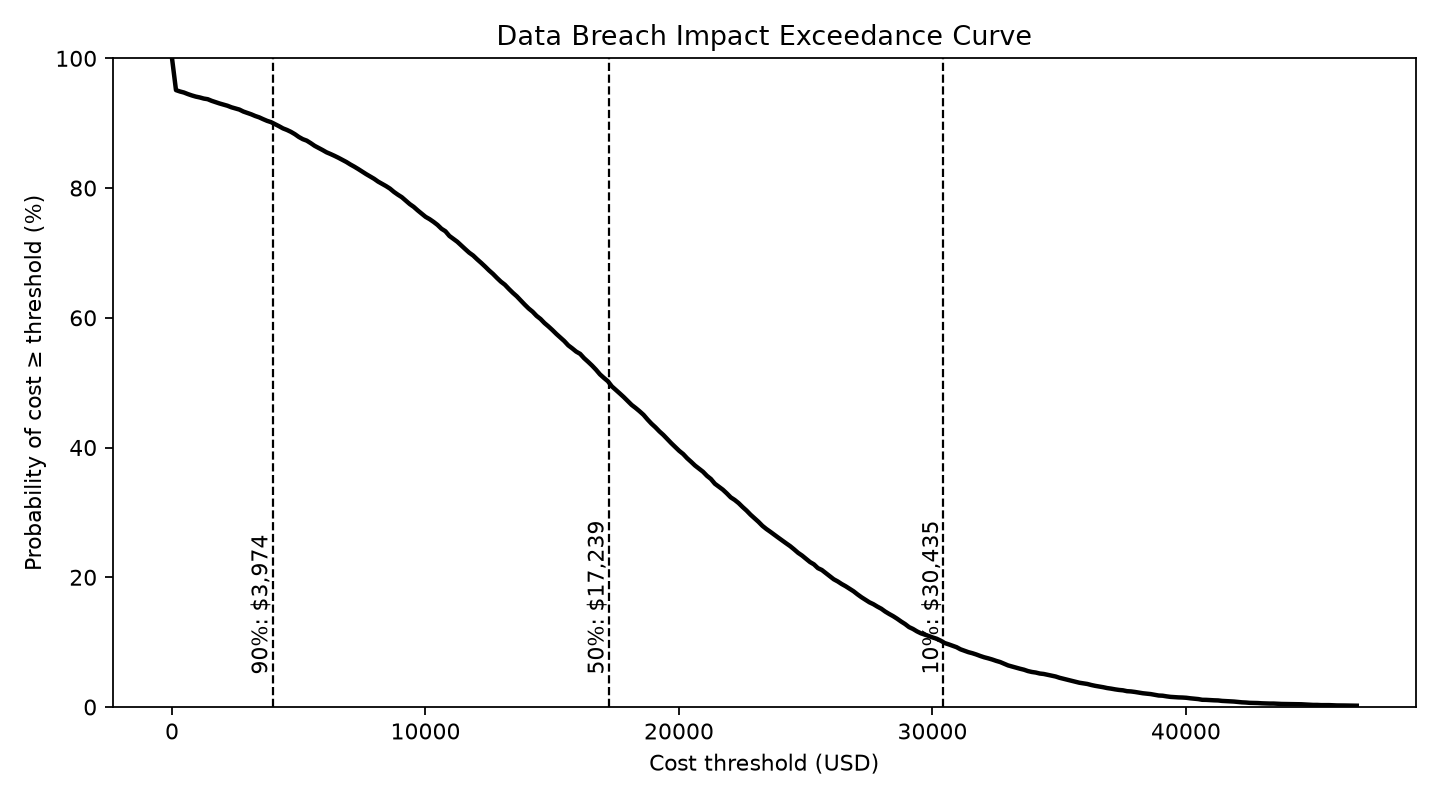
\includegraphics[width=\linewidth]{figures/percent_dataBreach_impact.png}}}
  \[
\mathrm{CI}_{80\%}(\theta) = [\$3{,}824, \$30{,}365]
\]
  \caption{A\index{Monte Carlo simulation} Monte Carlo simulation with a normal distribution suggests that there is a 90\% probability that\index{data breach} data breach events will cost \$3{,}824 or more in a year.  There is a 50\% likelihood that they will cost \$17{,}120 or more in a year.  There is a 10\% chance that they will cost \$30{,}365 or more in a year. \protect\endnote{\index{sample} sample size was set equivalent to the City of\index{Chattanooga} Chattanooga to determine the per capita rates for each year over data from \index{American Samoa} American Samoa and\index{California} California.  The means of those rates were used to set 10\% and 90\%\index{confidence interval} confidence intervals with \index{American Samoa} American Samoa and\index{California} California representing low and high \index{cybercrime} cybercrime impact values respectively.}
  \protect\endnote{Monte Carlo Modeling Toolkit authored by Derek E. Brink, \gls{cissp}, \url{www.linkedin.com/in/derekbrink}. March 2023.}
  }
  \label{fig:screenshot-montecarlo-\gls{databreach}-impact-percent}
\end{figure}
%%%%%%%%%%%%%%%%%%%% PERSONAL DATA BREACH %%%%%%%%%%%%%%%%%%%%
\newpage
\subsection{Personal Data Breach}\label{sec:persdatabreach}
\subsubsection{Lower Bound Computation}
\[
\begin{bmatrix}
\mathbf{x}_{\text{American Samoa}}^{(\text{count})}\\
\mathbf{x}_{\text{American Samoa}}^{(\text{dollars})}
\end{bmatrix}
=
\begin{bmatrix}
2 & \cdots & 1 & \cdots & 3\\
\$0 & \cdots & \$0 & \cdots & \$11
\end{bmatrix}.
\]
\[
\begin{bmatrix}
\mathbf{x}_{\text{American Samoa}}^{(\text{count scaled to sample population})}\\
\mathbf{x}_{\text{American Samoa}}^{(\text{dollars scaled to sample population})}
\end{bmatrix}
=
\begin{bmatrix}
6 & \cdots & 3 & \cdots & 11.42\\
\$0 & \cdots & \$0 & \cdots & \$0
\end{bmatrix}.
\]
  \[
\bar{X}_{\text{American Samoa}}^{(m)}
= \frac{1}{N}\sum_{i=1}^{N} X_{\text{American Samoa},i}^{(m)},
\]
\\
\[
\qquad
m \in \{\text{scaled count},\text{scaled dollars}\}
\]
\[
\begin{bmatrix}
\bar{X}_{\text{American Samoa}}^{(\text{scaled count})}\\
\bar{X}_{\text{American Samoa}}^{(\text{scaled dollars})}
\end{bmatrix}
=
\begin{bmatrix}
5.35\\
\$270.50
\end{bmatrix}.
\]
\subsubsection{Upper Bound Computation}
\[
\begin{bmatrix}
\mathbf{x}_{\text{California}}^{(\text{count})}\\
\mathbf{x}_{\text{California}}^{(\text{dollars})}
\end{bmatrix}
=
\begin{bmatrix}
4{,}031 & \cdots & 4{,}764 & \cdots & 8{,}196\\
\$8{,}808{,}240 & \cdots & \$9{,}355{,}626 & \cdots & \$153{,}022{,}651
\end{bmatrix}.
\]
\[
\begin{bmatrix}
\mathbf{x}_{\text{California}}^{(\text{count scaled to sample population})}\\
\mathbf{x}_{\text{California}}^{(\text{dollars scaled to sample population})}
\end{bmatrix}
=
\begin{bmatrix}
18 & \cdots & 21 & \cdots & 38.56\\
\$39{,}332.26 & \cdots & \$41{,}240.16 & \cdots & \$709{,}475.44
\end{bmatrix}.
\]
\[
\bar{X}_{\text{California}}^{(m)}
= \frac{1}{N}\sum_{i=1}^{N} X_{\text{California},i}^{(m)},
\]
\\
\[
\qquad
m \in \{\text{scaled count},\text{scaled dollars}\}
\]
\[
\begin{bmatrix}
\bar{X}_{\text{California}}^{(\text{scaled count})}\\
\bar{X}_{\text{California}}^{(\text{scaled dollars})}
\end{bmatrix}
=
\begin{bmatrix}
28.51\\
\$212{,}708.42
\end{bmatrix}.
\]
\subsubsection{Monte Carlo Simulations for Likelihood and Impact}
\begin{figure}[H]
  \centering
  \rotatebox{0}{\scalebox{1}{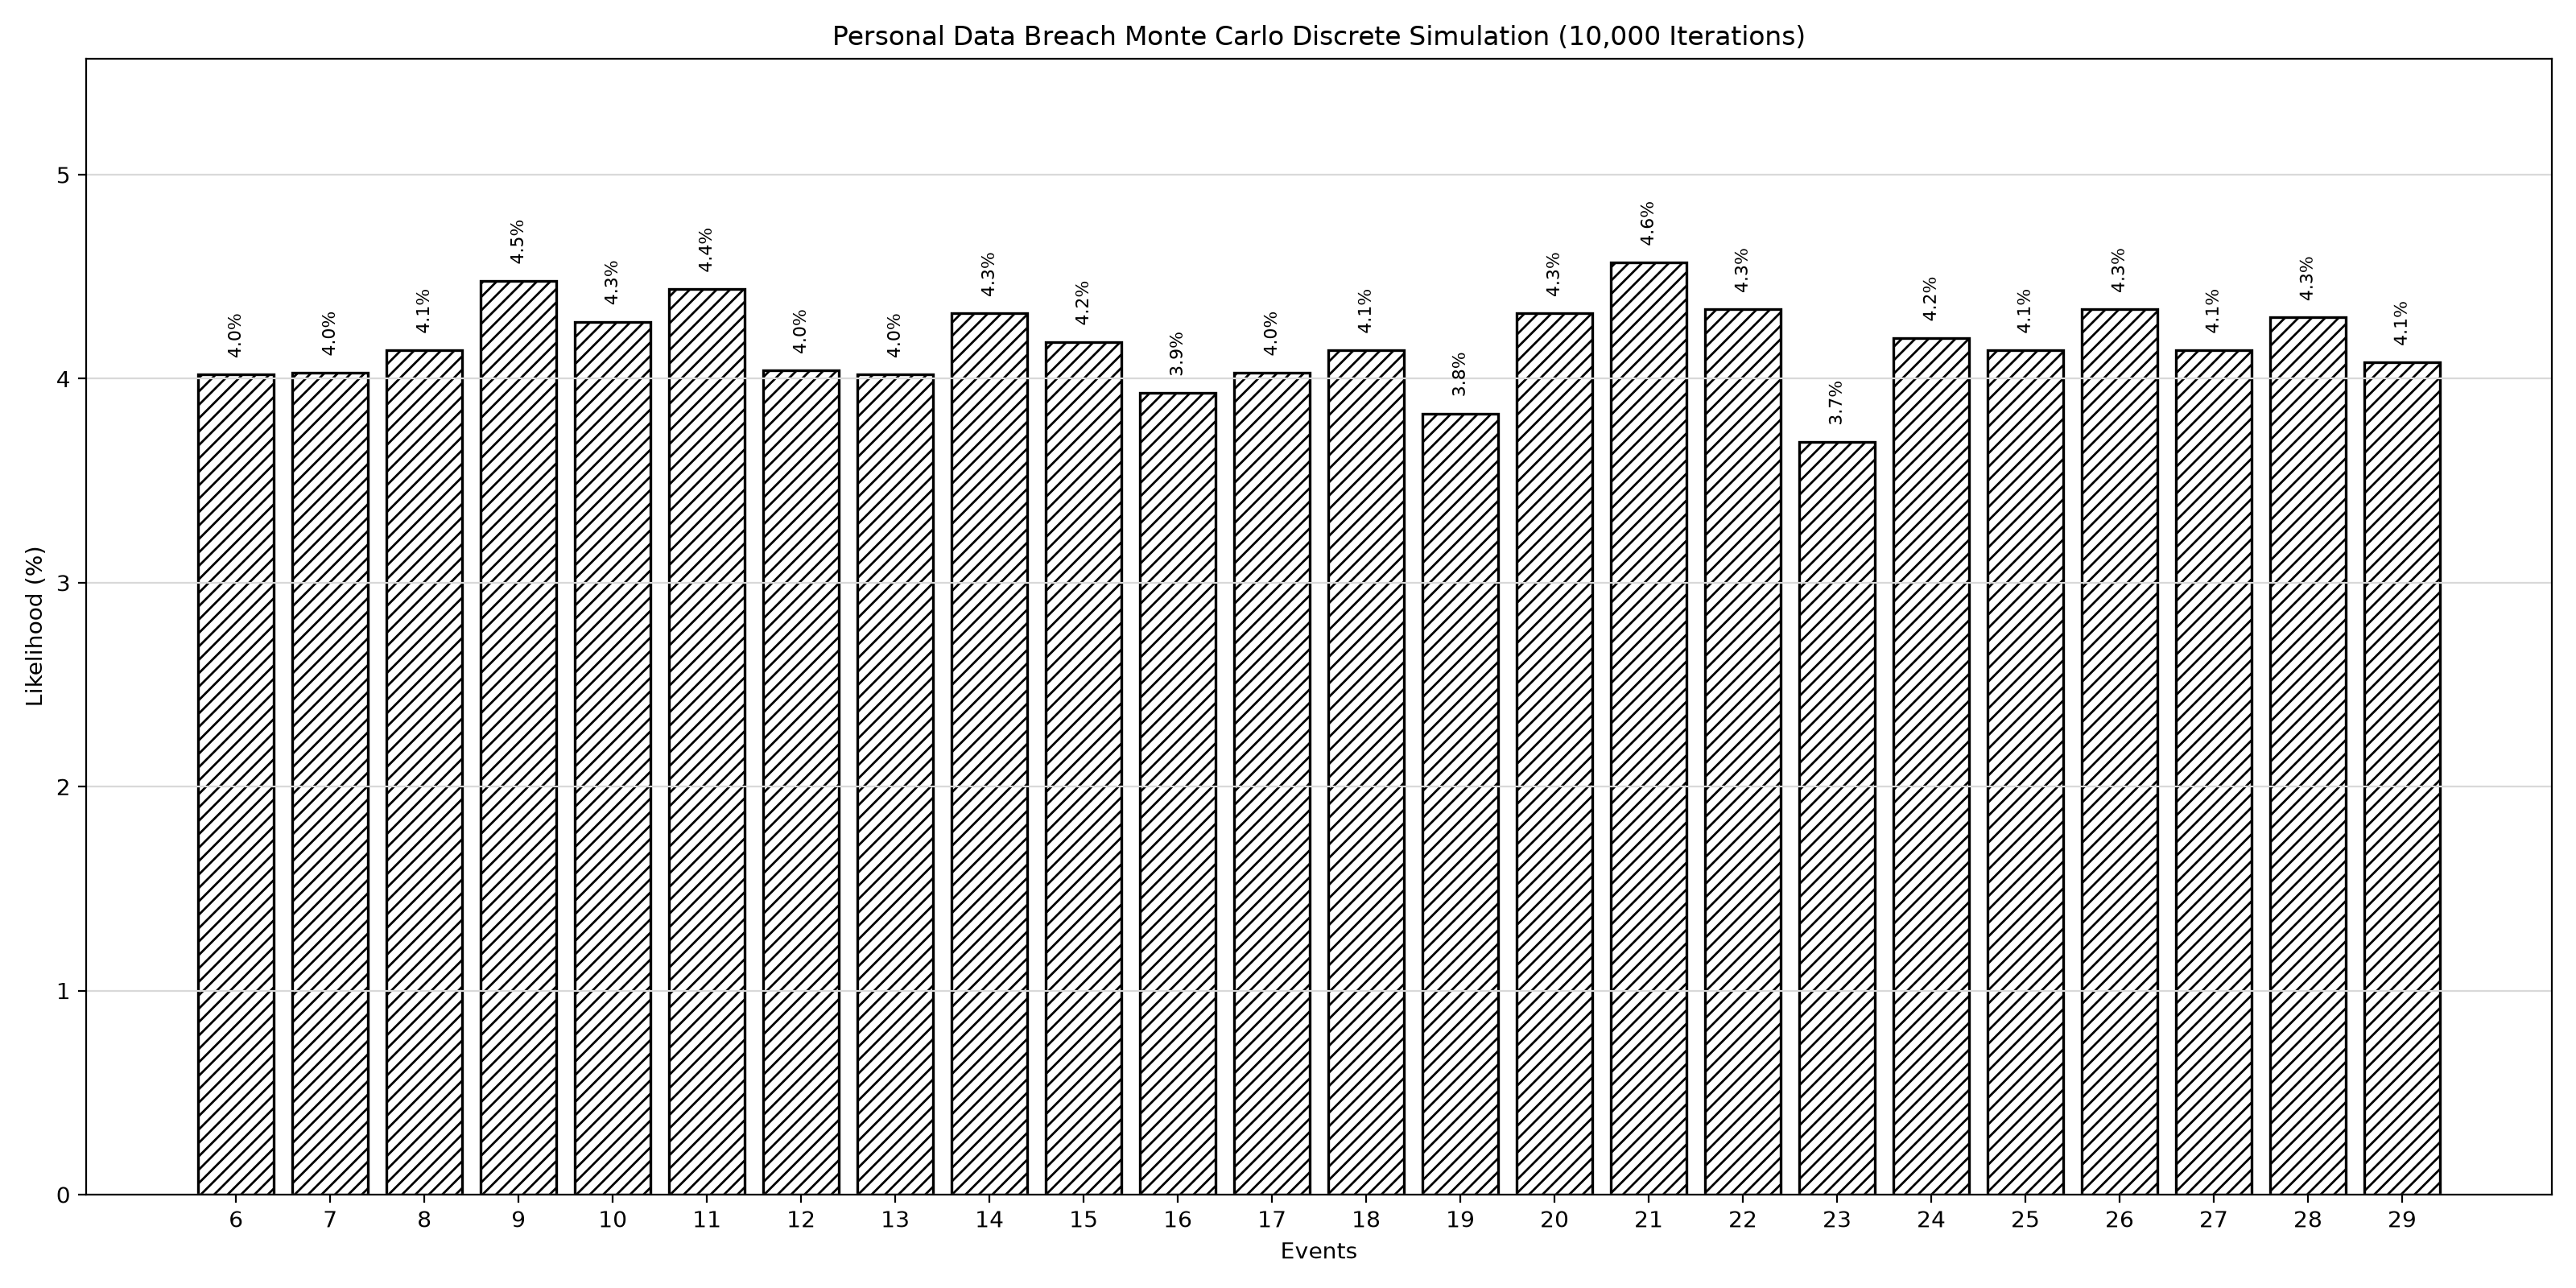
\includegraphics[width=\linewidth]{figures/discrete_persDataBreach_count.png}}}
  \caption{We ran a\index{Monte Carlo simulation} Monte Carlo simulation of 10{,}000 iterations with a discrete distribution to spread random instances between upper and lower bounds taken from the means of seven year samples. We bounded between 6 and 29 possible \index{personal data breach}personal \gls{databreach} events over a year.\protect\endnote{\index{sample} Sample size was set equivalent to the City of\index{Chattanooga} Chattanooga to determine the per capita rates for each year over data from \index{American Samoa} American Samoa and\index{California} California.  The means of those rates were used to set upper and lower bounds with \index{American Samoa} American Samoa and\index{California} California representing low and high \index{cybercrime} \gls{cybercrime} counts respectively.}
  \protect\endnote{Monte Carlo Modeling Toolkit authored by Derek E. Brink, \gls{cissp}, \url{www.linkedin.com/in/derekbrink}. March 2023.}
  }
  \label{fig:screenshot-montecarlo-persdatabreach-count-discrete}
\end{figure}
When we computed the upper and lower bounds, we recognized that a normal distribution would not fit well for forecasting likelihood.  We took the mean of the sample from American Samoa for the lower bound (5.35, rounded to 6); we took the mean from the sample from California for the upper bound (28.51, rounded to 29); we had a separation of 23 units.  Therefore, we switched to a discrete model with all 24 options sharing an equal likelihood.
\begin{table}[H]
  \centering
  \caption{Monte Carlo Discrete Simulation Values for Personal \gls{databreach}}
  \label{tab:discrete_persdatabreach_montecarlo}
  \begin{center}
\begin{tabular}{@{}>{\centering\arraybackslash}p{0.20\linewidth} >{\centering\arraybackslash}p{0.10\linewidth} >{\centering\arraybackslash}p{0.10\linewidth} >{\centering\arraybackslash}p{0.10\linewidth} >{\centering\arraybackslash}p{0.10\linewidth} >{\centering\arraybackslash}p{0.10\linewidth} >{\centering\arraybackslash}p{0.10\linewidth}}
    \toprule
Events
  &6
  &7
  &8
  &9
  &10
  &11\\
    \midrule
Likelihood
  &4.0\%
  &4.0\%
  &4.1\%
  &4.5\%
  &4.3\%
  &4.4\%\\
    \bottomrule \end{tabular}
\begin{tabular}{@{}>{\centering\arraybackslash}p{0.20\linewidth} >{\centering\arraybackslash}p{0.10\linewidth} >{\centering\arraybackslash}p{0.10\linewidth} >{\centering\arraybackslash}p{0.10\linewidth} >{\centering\arraybackslash}p{0.10\linewidth} >{\centering\arraybackslash}p{0.10\linewidth} >{\centering\arraybackslash}p{0.10\linewidth}}
    \toprule
Events
  &12
  &13
  &14
  &15
  &16
  &17\\
    \midrule
Likelihood
  &4.0\%
  &4.0\%
  &4.3\%
  &4.2\%
  &3.9\%
  &4.0\%\\
    \bottomrule \end{tabular}
\begin{tabular}{@{}>{\centering\arraybackslash}p{0.20\linewidth} >{\centering\arraybackslash}p{0.10\linewidth} >{\centering\arraybackslash}p{0.10\linewidth} >{\centering\arraybackslash}p{0.10\linewidth} >{\centering\arraybackslash}p{0.10\linewidth} >{\centering\arraybackslash}p{0.10\linewidth} >{\centering\arraybackslash}p{0.10\linewidth}}
    \toprule
Events
  &18
  &19
  &20
  &21
  &22
  &23\\
    \midrule
Likelihood
  &4.1\%
  &3.8\%
  &4.3\%
  &4.6\%
  &4.3\%
  &3.7\%\\
    \bottomrule \end{tabular}
\begin{tabular}{@{}>{\centering\arraybackslash}p{0.20\linewidth} >{\centering\arraybackslash}p{0.10\linewidth} >{\centering\arraybackslash}p{0.10\linewidth} >{\centering\arraybackslash}p{0.10\linewidth} >{\centering\arraybackslash}p{0.10\linewidth} >{\centering\arraybackslash}p{0.10\linewidth} >{\centering\arraybackslash}p{0.10\linewidth}}
    \toprule
Events
  &24
  &25
  &26
  &27
  &28
  &29\\
    \midrule
Likelihood
  &4.2\%
  &4.1\%
  &4.3\%
  &4.1\%
  &4.3\%
  &4.1\%\\
    \bottomrule \end{tabular}
    \end{center}
  \raggedright{A\index{Monte Carlo simulation} Monte Carlo simulation was run using a discrete distribution.  We bounded the simulation between 6 and 29 events.  We assigned an approximately 4.2\% likelihood to each bin.  A representative 10{,}000-iteration simulation produced the percentages shown above, with no unused event bins.}
\end{table}

\begin{figure}[H]
  \centering
  \rotatebox{0}{\scalebox{1}{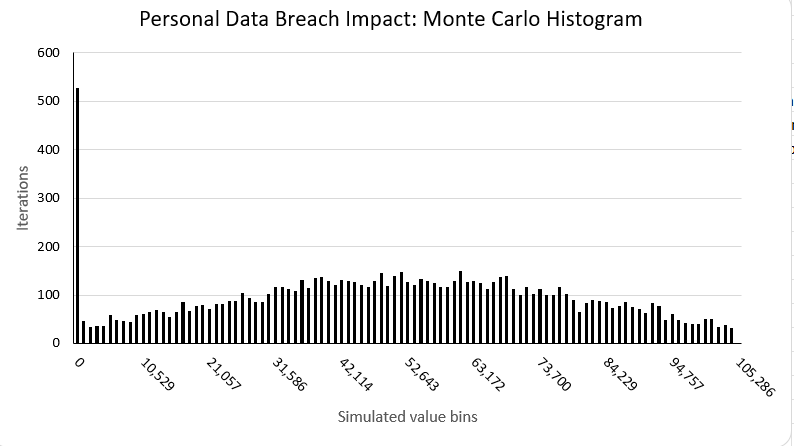
\includegraphics[width=\linewidth]{figures/histogram_persDataBreach_impact.png}}}
  \caption{We ran a\index{Monte Carlo simulation} Monte Carlo simulation of 10{,}000 iterations with a normal distribution to spread random instances between bounds taken from means of seven year samples. We set a lower bound that the events would cost at \$270.50.  We set an upper bound that the events would cost \$212{,}708.42.\protect\endnote{\index{sample} Sample size was set equivalent to the City of\index{Chattanooga} Chattanooga to determine the per capita rates for each year over data from \index{American Samoa} American Samoa and\index{California} California.  The means of those rates were used to set upper and lower bounds with \index{American Samoa} American Samoa and\index{California} California representing low and high \index{cybercrime} \gls{cybercrime} impact values respectively.}
  \protect\endnote{Monte Carlo Modeling Toolkit authored by Derek E. Brink, \gls{cissp}, \url{www.linkedin.com/in/derekbrink}. March 2023.}
  }
  \label{fig:screenshot-montecarlo-persdatabreach-impact-histo}
\end{figure}
\begin{figure}[H]
  \centering
  \rotatebox{0}{\scalebox{1}{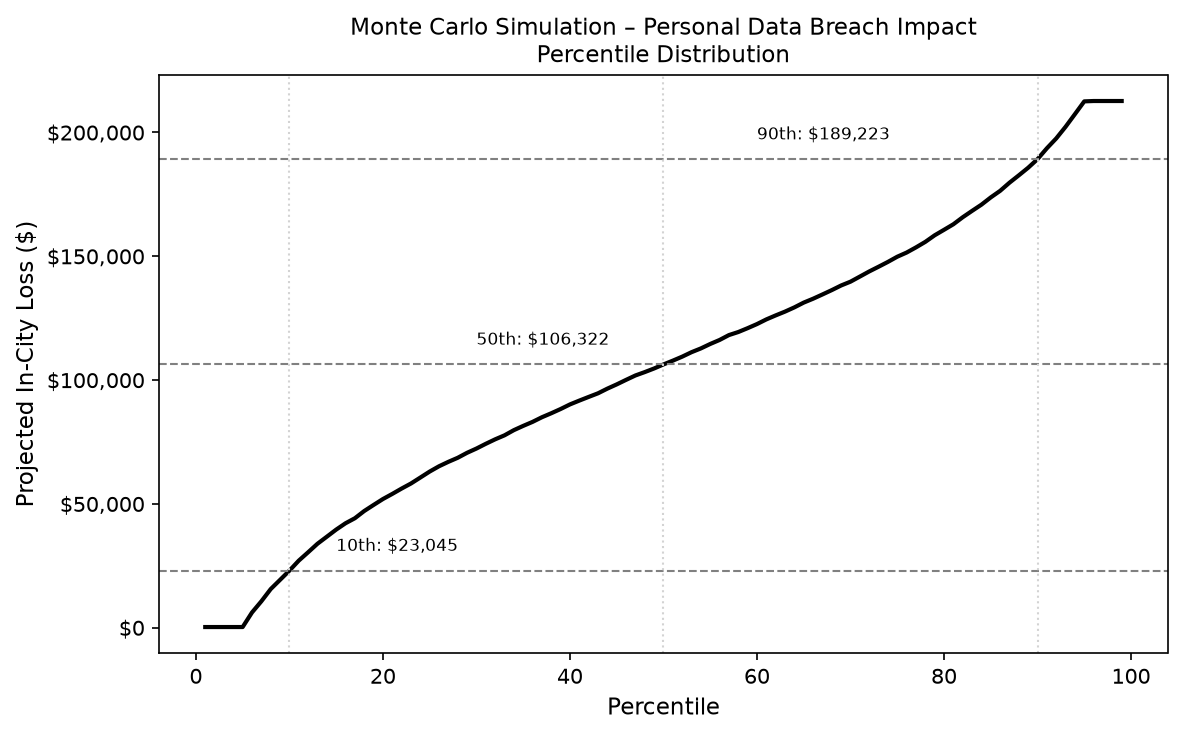
\includegraphics[width=\linewidth]{figures/percent_persDataBreach_impact.png}}}
  \[
\mathrm{CI}_{80\%}(\theta) = [\$23{,}045, \$189{,}223]
\]
  \caption{A\index{Monte Carlo simulation} Monte Carlo simulation with a normal distribution suggests that there is a 90\% probability that\index{personal data breach} personal data breach events will cost \$23{,}045 or more in a year.  There is a 50\% likelihood that they will cost \$106{,}322 or more in a year.  There is a 10\% chance that they will cost \$189{,}223 or more in a year. \protect\endnote{\index{sample} sample size was set equivalent to the City of\index{Chattanooga} Chattanooga to determine the per capita rates for each year over data from \index{American Samoa} American Samoa and\index{California} California.  The means of those rates were used to set 10\% and 90\%\index{confidence interval} confidence intervals with \index{American Samoa} American Samoa and\index{California} California representing low and high \index{cybercrime} cybercrime impact values respectively.}
  \protect\endnote{Monte Carlo Modeling Toolkit authored by Derek E. Brink, \gls{cissp}, \url{www.linkedin.com/in/derekbrink}. March 2023.}
  }
  \label{fig:screenshot-montecarlo-persdatabreach-impact-percent}
\end{figure}


\subsubsection{Threats to System Intrusion}
\begin{table}[H]
  \centering
  \caption{Projected In-City Victim Counts, City of\index{Chattanooga} Chattanooga, Threats to System Intrusion}
  \label{tab:chattanoogacrime3}
  \begin{tabular}{@{}>{\centering\arraybackslash}p{0.05\linewidth} >{\centering\arraybackslash}
  p{0.25\linewidth} >{\centering\arraybackslash}
  p{0.25\linewidth} >{\centering\arraybackslash}
  p{0.25\linewidth} >{\centering\arraybackslash}
  p{0.05\linewidth}}
    \toprule
    Year
    &Malware\index{malware}
    &Phishing\index{phishing}
    &Ransomware\index{ransomware}
    &\\
    \midrule


2016&1&7&1&\endnote{original\protect\url{https://www.ic3.gov/Media/PDF/AnnualReport/2016State/StateReport.aspx\#?s=47} current \protect\url{https://www.ic3.gov/AnnualReport/Reports/2016_IC3Report.pdf}}\\
2017&1&9&0&\endnote{original:\protect\url{https://www.ic3.gov/Media/PDF/AnnualReport/2017State/StateReport.aspx\#?s=47} current: \url{https://www.ic3.gov/AnnualReport/Reports/2017_IC3Report.pdf}}\\
2018&0&8&0&\endnote{original:\protect\url{https://www.ic3.gov/Media/PDF/AnnualReport/2018State/StateReport.aspx\#?s=47} current: \url{https://www.ic3.gov/AnnualReport/Reports/2018_IC3Report.pdf}}\\
2019&1&8&0&\endnote{original:\protect\url{https://www.ic3.gov/Media/PDF/AnnualReport/2019State/StateReport.aspx\#?s=47} current: \url{https://www.ic3.gov/AnnualReport/Reports/2019_IC3Report.pdf}}\\
2020&0&9&0&\endnote{original:\protect\url{https://www.ic3.gov/Media/PDF/AnnualReport/2020State/StateReport.aspx\#?s=47} current: \url{https://www.ic3.gov/AnnualReport/Reports/2020_IC3Report.pdf}}\\
2021&0&11&1&\endnote{original:\protect\url{https://www.ic3.gov/Media/PDF/AnnualReport/2021State/StateReport.aspx\#?s=47} current: \url{https://www.ic3.gov/AnnualReport/Reports/2021_IC3Report.pdf}}\\
2022&0&7&0&\endnote{original:\protect\url{https://www.ic3.gov/Media/PDF/AnnualReport/2022State/StateReport.aspx\#?s=47} current: \url{https://www.ic3.gov/AnnualReport/Reports/2022_IC3Report.pdf}}\\

    \bottomrule \end{tabular}
  \raggedright{Counts deduced from \gls{ic3} Victim Complaints for Tennessee adjusted for a per-capita rate and then multiplied by the city's \index{population} population for that year.}
\end{table}
%%%%%%%%%%%%%%%%%%%%  MALWARE\index{malware} %%%%%%%%%%%%%%%%%%%%%%%%
\newpage
\subsection{Malware}
\subsubsection{Lower Bound Computation}
\[
\begin{bmatrix}
\mathbf{x}_{\text{American Samoa}}^{(\text{count})}\\
\mathbf{x}_{\text{American Samoa}}^{(\text{dollars})}
\end{bmatrix}
=
\begin{bmatrix}
0 & 0 & \cdots & 0\\
\$0 &\$0 & \cdots &\$0 
\end{bmatrix}.
\]
\[
\begin{bmatrix}
\mathbf{x}_{\text{American Samoa}}^{(\text{count scaled to sample population})}\\
\mathbf{x}_{\text{American Samoa}}^{(\text{dollars scaled to sample population})}
\end{bmatrix}
=
\begin{bmatrix}
0 & \cdots & 0\\
\$0 & \cdots &\$0
\end{bmatrix}.
\]
  \[
\bar{X}_{\text{American Samoa}}^{(m)}
= \frac{1}{N}\sum_{i=1}^{N} X_{\text{American Samoa},i}^{(m)},
\]
\\
\[
\qquad
m \in \{\text{scaled count},\text{scaled dollars}\}
\]
\[
\begin{bmatrix}
\bar{X}_{\text{American Samoa}}^{(\text{scaled count})}\\
\bar{X}_{\text{American Samoa}}^{(\text{scaled dollars})}
\end{bmatrix}
=
\begin{bmatrix}
0.86\\
\$0
\end{bmatrix}.
\]
\subsubsection{Upper Bound Computation}
\[
\begin{bmatrix}
\mathbf{x}_{\text{California}}^{(\text{count})}\\
\mathbf{x}_{\text{California}}^{(\text{dollars})}
\end{bmatrix}
=
\begin{bmatrix}
347 & 408 & \cdots & 94\\
\$1{,}617{,}528 &\$400{,}701  & \cdots &\$0 
\end{bmatrix}.
\]
\[
\begin{bmatrix}
\mathbf{x}_{\text{California}}^{(\text{count scaled to sample population})}\\
\mathbf{x}_{\text{California}}^{(\text{dollars scaled to sample population})}
\end{bmatrix}
=
\begin{bmatrix}
1 & 1 & \cdots & 0\\
\$4{,}661 &\$982 & \cdots &\$0
\end{bmatrix}.
\]
\[
\bar{X}_{\text{California}}^{(m)}
= \frac{1}{N}\sum_{i=1}^{N} X_{\text{California},i}^{(m)},
\]
\\
\[
\qquad
m \in \{\text{scaled count},\text{scaled dollars}\}
\]
\[
\begin{bmatrix}
\bar{X}_{\text{California}}^{(\text{scaled count})}\\
\bar{X}_{\text{California}}^{(\text{scaled dollars})}
\end{bmatrix}
=
\begin{bmatrix}
0.63\\
\$1{,}013
\end{bmatrix}.
\]
\subsubsection{Monte Carlo Simulations for Likelihood and Impact}
\begin{figure}[H]
  \centering
  \rotatebox{0}{\scalebox{1}{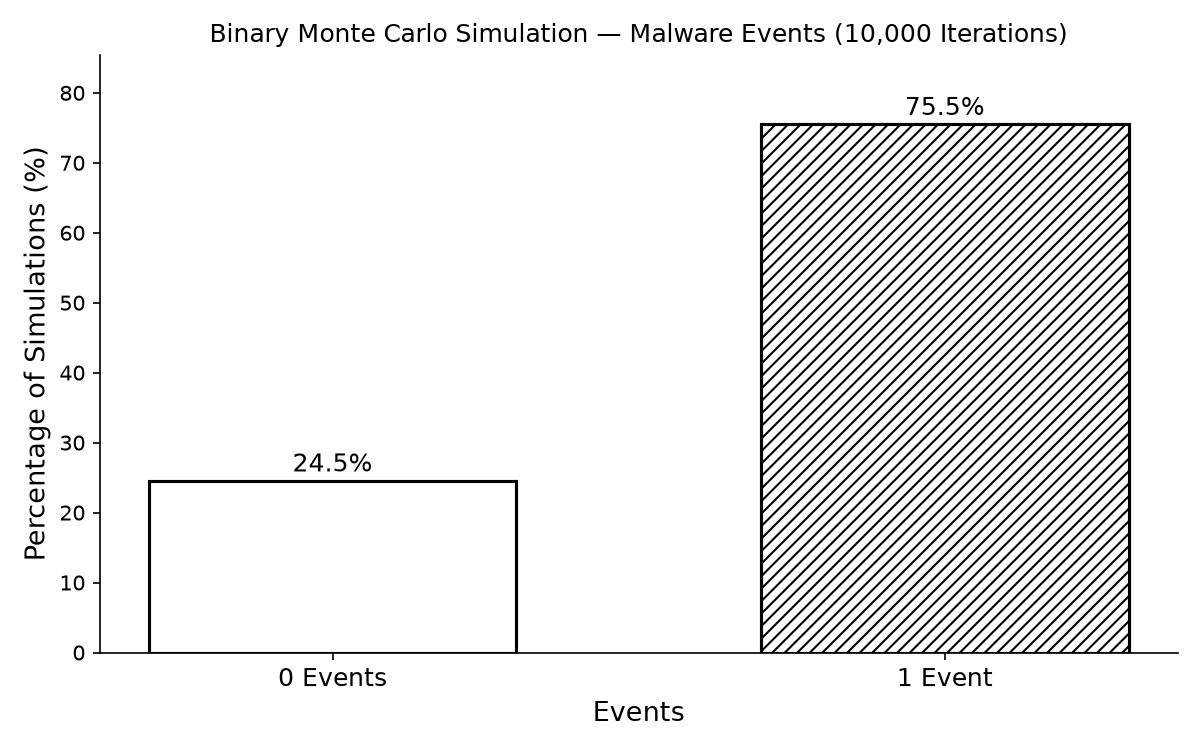
\includegraphics[width=\linewidth]{figures/binary_malware_count.png}}}
  \caption{We ran a\index{Monte Carlo simulation} Monte Carlo simulation of 10,000 iterations with a \gls{binary} distribution to spread random instances between upper and lower bounds taken from the means of seven year samples. We bounded between 0 and 1 possible\index{malware} \gls{malware} events over a year.\protect\endnote{\index{sample} Sample size was set equivalent to the City of\index{Chattanooga} Chattanooga to determine the per capita rates for each year over data from \index{American Samoa} American Samoa and\index{California} California.  The means of those rates were used to set upper and lower bounds with \index{American Samoa} American Samoa and\index{California} California representing the range of likely \index{malware} \gls{malware} counts respectively.}
  \protect\endnote{Monte Carlo Modeling Toolkit authored by Derek E. Brink, \gls{cissp}, \url{www.linkedin.com/in/derekbrink}. March 2023.}
  }
  \label{fig:screenshot-montecarlo-\gls{malware}-count-binary}
\end{figure}
When we computed the upper and lower bounds, we recognized that a normal distribution would not fit well for forecasting likelihood.  We took the mean of the sample from American Samoa for the lower bound (0.86); we took the mean from the sample from California for the upper bound (0.63); we had a separation of approximately 1 unit.  Because both means fall between 0 and 1, we used a \gls{binary} model with two options (0 and 1 events) sharing a combined likelihood of 100\%.
\begin{table}[H]
  \centering
  \caption{Monte Carlo \gls{binary} Simulation Values for \gls{malware}}
  \label{tab:binary_malware_montecarlo}
  \begin{center}
  \begin{tabular}{@{}>{\centering\arraybackslash}
  p{0.20\linewidth} >{\centering\arraybackslash}
  p{0.20\linewidth} >{\centering\arraybackslash}
  p{0.20\linewidth}}
    \toprule
Events
&0
&1\\
    \midrule
Likelihood    
&24.5\%
&75.5\%\\
    \bottomrule \end{tabular}
    \end{center}
  \raggedright{A\index{Monte Carlo simulation} Monte Carlo simulation was run using a \gls{binary} distribution.  We bounded the simulation between 0 and 1 events.  We assigned an approximately 74.6\% likelihood to the 1-event bin.  The resulting distribution showed the effect of randomness on each possible outcome.}
\end{table}

\begin{figure}[H]
  \centering
  \rotatebox{0}{\scalebox{1}{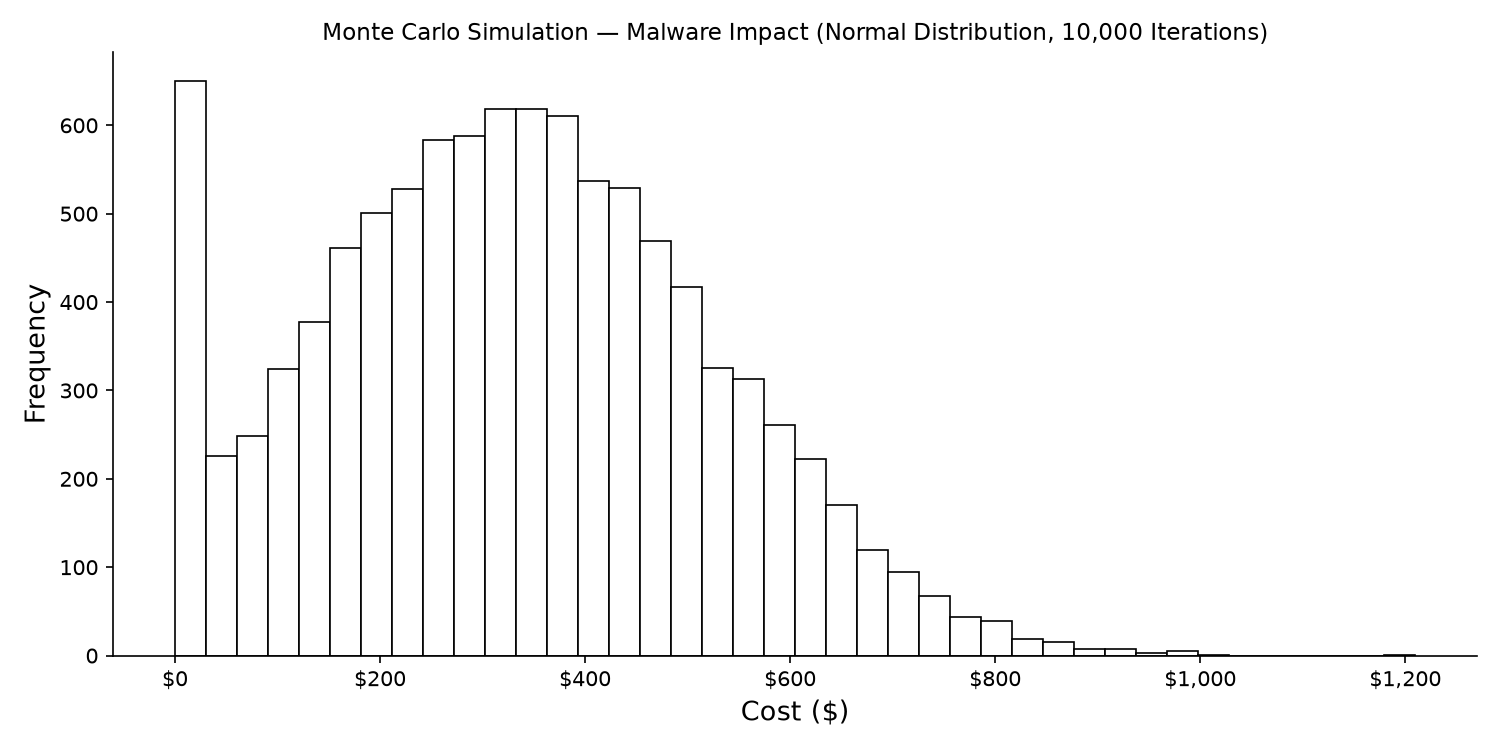
\includegraphics[width=\linewidth]{figures/histogram_malware_impact_v2.png}}}
  \caption{We ran a\index{Monte Carlo simulation} Monte Carlo simulation of 10,000 iterations with a normal distribution to spread random instances between bounds taken from means of seven year samples.  We set a lower bound that the events would cost at \$0.  We set an upper bound that the events would cost \$649.99.  \protect\endnote{\index{sample} Sample size was set equivalent to the City of\index{Chattanooga} Chattanooga to determine the per capita rates for each year over data from \index{American Samoa} American Samoa and\index{California} California.  The means of those rates were used to set upper and lower bounds with \index{American Samoa} American Samoa and\index{California} California representing low and high \index{malware} \gls{malware} impact values respectively.}
  \protect\endnote{Monte Carlo Modeling Toolkit authored by Derek E. Brink, \gls{cissp}, \url{www.linkedin.com/in/derekbrink}. March 2023.}
  }
  \label{fig:screenshot-montecarlo-malware\index{malware}-impact-histo}
\end{figure}
\begin{figure}[H]
  \centering
  \rotatebox{0}{\scalebox{1}{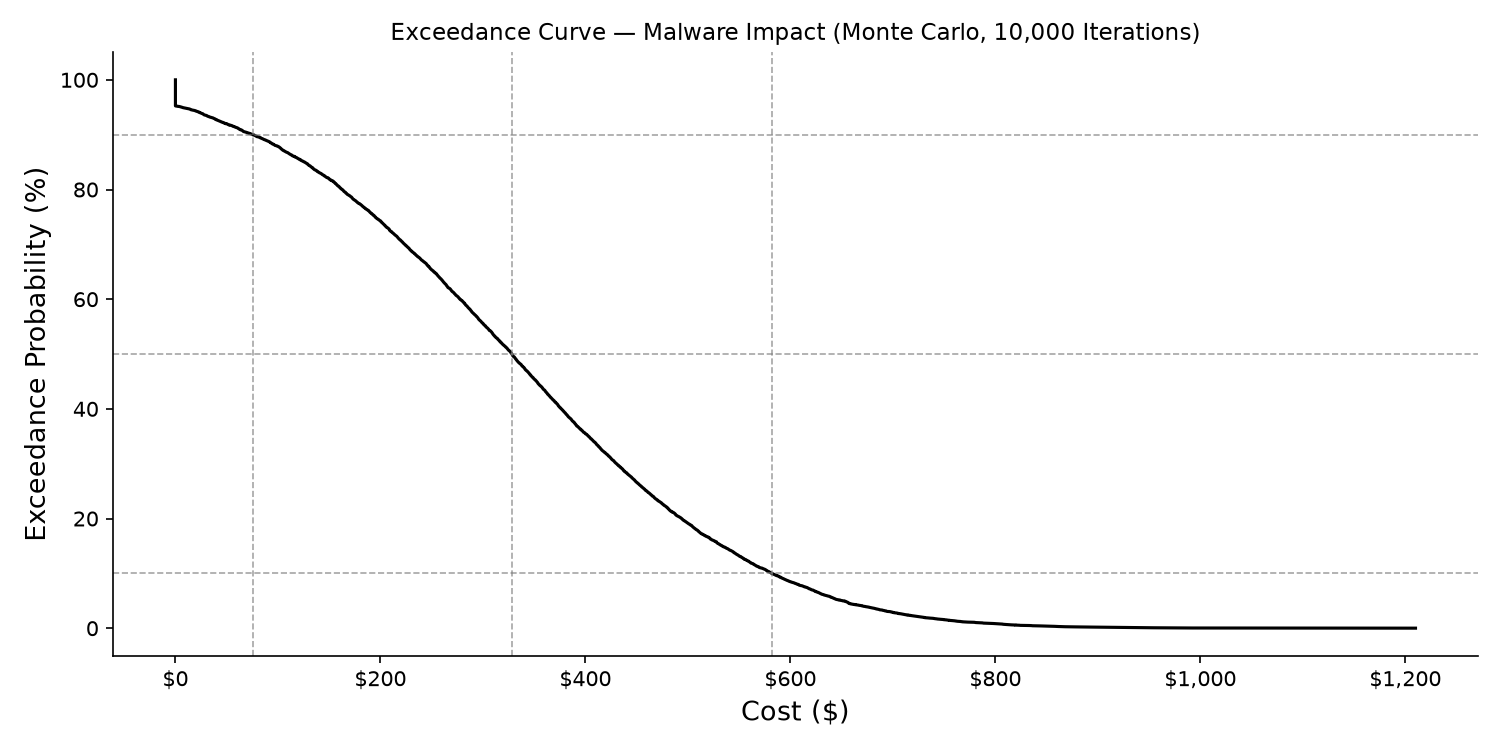
\includegraphics[width=\linewidth]{figures/percent_malware_impact_v2.png}}}
  \[
\mathrm{CI}_{80\%}(\theta) = [\$75.28, \$581.59]
\]
  \caption{A\index{Monte Carlo simulation} Monte Carlo simulation with a normal distribution suggests that there is a 90\% probability that\index{malware} malware events will cost \$75.28 or more in a year.  There is a 50\% likelihood that they will cost \$328.32 or more in a year.  There is a 10\% chance that they will cost \$581.59 or more in a year. \protect\endnote{\index{sample} sample size was set equivalent to the City of\index{Chattanooga} Chattanooga to determine the per capita rates for each year over data from \index{American Samoa} American Samoa and\index{California} California.  The means of those rates were used to set upper and lower bounds with \index{American Samoa} American Samoa and\index{California} California representing low and high \index{malware} malware impact values respectively.}
  \protect\endnote{Monte Carlo Modeling Toolkit authored by Derek E. Brink, \gls{cissp}, \url{www.linkedin.com/in/derekbrink}. March 2023.}
  }
  \label{fig:screenshot-montecarlo-malware\index{malware}-impact-percent}
\end{figure}

%%%%%%%%%%%%%%%%%%%%  PHISHING\index{phishing} %%%%%%%%%%%%%%%%%%%%%%%%
\newpage
\subsection{Phishing}\label{sec:phishing}
\subsubsection{Lower Bound Computation}
\[
\begin{bmatrix}
\mathbf{x}_{\text{American Samoa}}^{(\text{count})}\\
\mathbf{x}_{\text{American Samoa}}^{(\text{dollars})}
\end{bmatrix}
=
\begin{bmatrix}
1 & 1 & 0 & 1 & 1 & 1 & 1\\
\$0 &\$0 &\$0 &\$0 &\$0 &\$0 &\$0 
\end{bmatrix}.
\]
\[
\begin{bmatrix}
\mathbf{x}_{\text{American Samoa}}^{(\text{count scaled to sample population})}\\
\mathbf{x}_{\text{American Samoa}}^{(\text{dollars scaled to sample population})}
\end{bmatrix}
=
\begin{bmatrix}
3 & \cdots & 3\\
\$0 & \cdots &\$0
\end{bmatrix}.
\]
  \[
\bar{X}_{\text{American Samoa}}^{(m)}
= \frac{1}{N}\sum_{i=1}^{N} X_{\text{American Samoa},i}^{(m)},
\]
\\
\[
\qquad
m \in \{\text{scaled count},\text{scaled dollars}\}
\]
\[
\begin{bmatrix}
\bar{X}_{\text{American Samoa}}^{(\text{scaled count})}\\
\bar{X}_{\text{American Samoa}}^{(\text{scaled dollars})}
\end{bmatrix}
=
\begin{bmatrix}
3\\
\$0
\end{bmatrix}.
\]
\subsubsection{Upper Bound Computation}
\[
\begin{bmatrix}
\mathbf{x}_{\text{California}}^{(\text{count})}\\
\mathbf{x}_{\text{California}}^{(\text{dollars})}
\end{bmatrix}
=
\begin{bmatrix}
2,059 & 3,302 & \cdots & 2,041\\
\$11,073,447 &\$8,864,419  & \cdots &\$14,628,440 
\end{bmatrix}.
\]
\[
\begin{bmatrix}
\mathbf{x}_{\text{California}}^{(\text{count scaled to sample population})}\\
\mathbf{x}_{\text{California}}^{(\text{dollars scaled to sample population})}
\end{bmatrix}
=
\begin{bmatrix}
9 & 15 & \cdots & 15\\
\$48,402 &\$40,268 & \cdots &\$64,505 
\end{bmatrix}.
\]
\[
\bar{X}_{\text{California}}^{(m)}
= \frac{1}{N}\sum_{i=1}^{N} X_{\text{California},i}^{(m)},
\]
\\
\[
\qquad
m \in \{\text{scaled count},\text{scaled dollars}\}
\]
\[
\begin{bmatrix}
\bar{X}_{\text{California}}^{(\text{scaled count})}\\
\bar{X}_{\text{California}}^{(\text{scaled dollars})}
\end{bmatrix}
=
\begin{bmatrix}
12\\
\$46,695
\end{bmatrix}.
\]
\subsubsection{Monte Carlo Simulations for Likelihood and Impact}
\begin{figure}[H]
  \centering
  \rotatebox{0}{\scalebox{1}{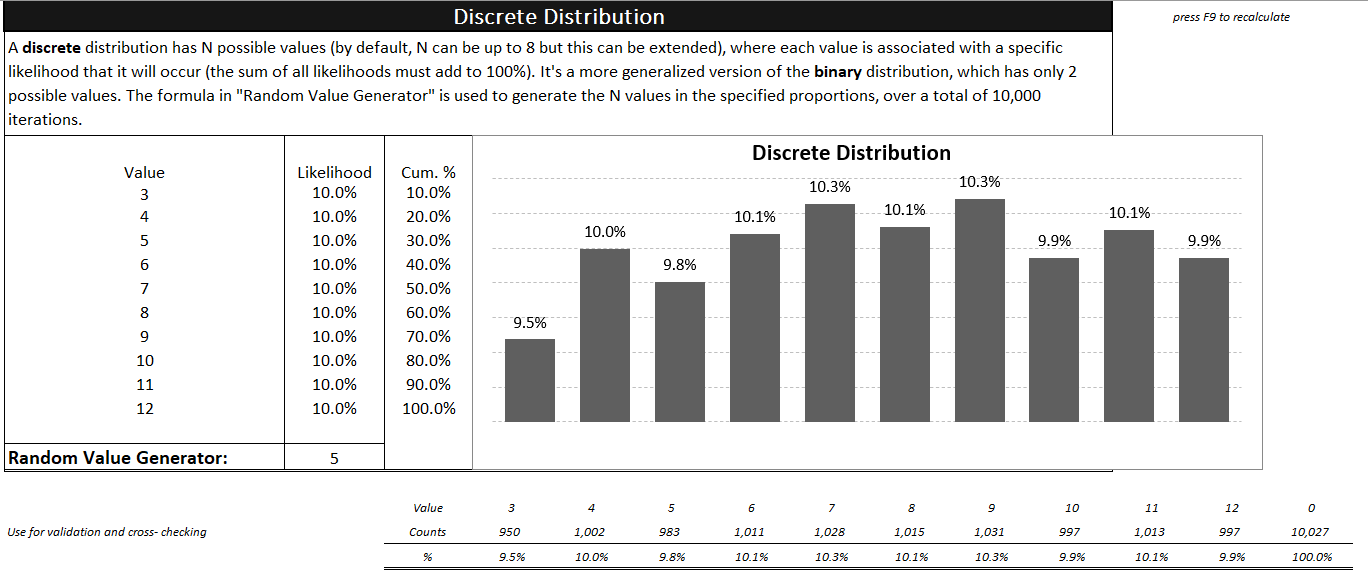
\includegraphics[width=\linewidth]{figures/discrete_phishing_count.png}}}
  \caption{We ran a\index{Monte Carlo simulation} Monte Carlo simulation of 10,000 iterations with a discrete distribution to spread random instances between confidence intervals taken from the means of seven year samples. We bounded between 3 and 12 possible \gls{phishing} events over a year.\protect\endnote{\index{sample} Sample size was set equivalent to the City of\index{Chattanooga} Chattanooga to determine the per capita rates for each year over data from \index{American Samoa} American Samoa and\index{California} California.  The medians of those rates were used to set 10\% and 90\%\index{confidence interval} confidence intervals with \index{American Samoa} American Samoa and\index{California} California representing low and high \index{cybercrime} cybercrime counts respectively.}
  \protect\endnote{Monte Carlo Modeling Toolkit authored by Derek E. Brink, \gls{cissp}, \url{www.linkedin.com/in/derekbrink}. March 2023.}
  }
  \label{fig:screenshot-montecarlo-phishing-count-discrete}
\end{figure}
When we computed the upper and lower bounds, we recognized that a normal distribution would not fit well for forecasting likelihood.  We took the mean of the sample from American Samoa for the lower bound (3); we took the mean from the sample from California for the upper bound (12); we had a separation of 9 units.  Therefore, we switched to a discrete model with all 10 options sharing an equal likelihood.
\begin{table}[H]
  \centering
  \caption{Monte Carlo Discrete Simulation Values for \gls{phishing}}
  \label{tab:discrete_phishing_montecarlo}
  \begin{center}
  \begin{tabular}{@{}>{\centering\arraybackslash}
  p{0.20\linewidth} >{\centering\arraybackslash}
  p{0.10\linewidth} >{\centering\arraybackslash}
  p{0.10\linewidth} >{\centering\arraybackslash}
  p{0.10\linewidth} >{\centering\arraybackslash}
  p{0.10\linewidth} >{\centering\arraybackslash}
  p{0.10\linewidth}}
    \toprule
Events
&3
&4
&5
&6
&7\\
    \midrule
Likelihood    
&10.4\%
&9.9\%
&9.7\%
&10.0\%
&10.1\%\\
    \bottomrule \end{tabular}
\begin{tabular}{@{}>{\centering\arraybackslash}
  p{0.20\linewidth} >{\centering\arraybackslash}
  p{0.10\linewidth} >{\centering\arraybackslash}
  p{0.10\linewidth} >{\centering\arraybackslash}
  p{0.10\linewidth} >{\centering\arraybackslash}
  p{0.10\linewidth} >{\centering\arraybackslash}
  p{0.10\linewidth}}
    \toprule
Events    
    &8
    &9
    &10
    &11
    &12\\
    \midrule
Likelihood
&10.2\%
&10.1\%
&9.9\%
&9.9\%
&9.9\%\\
    \bottomrule \end{tabular}
    \end{center}
  \raggedright{A\index{Monte Carlo simulation} Monte Carlo simulation was run using a discrete distribution.  We bounded the simulation between 3 and 12 events.  We assigned a 10\% likelihood to each bin.  The resulting distribution showed the effect of randomness on each possible outcome.}
\end{table}

\begin{figure}[H]
  \centering
  \rotatebox{0}{\scalebox{1}{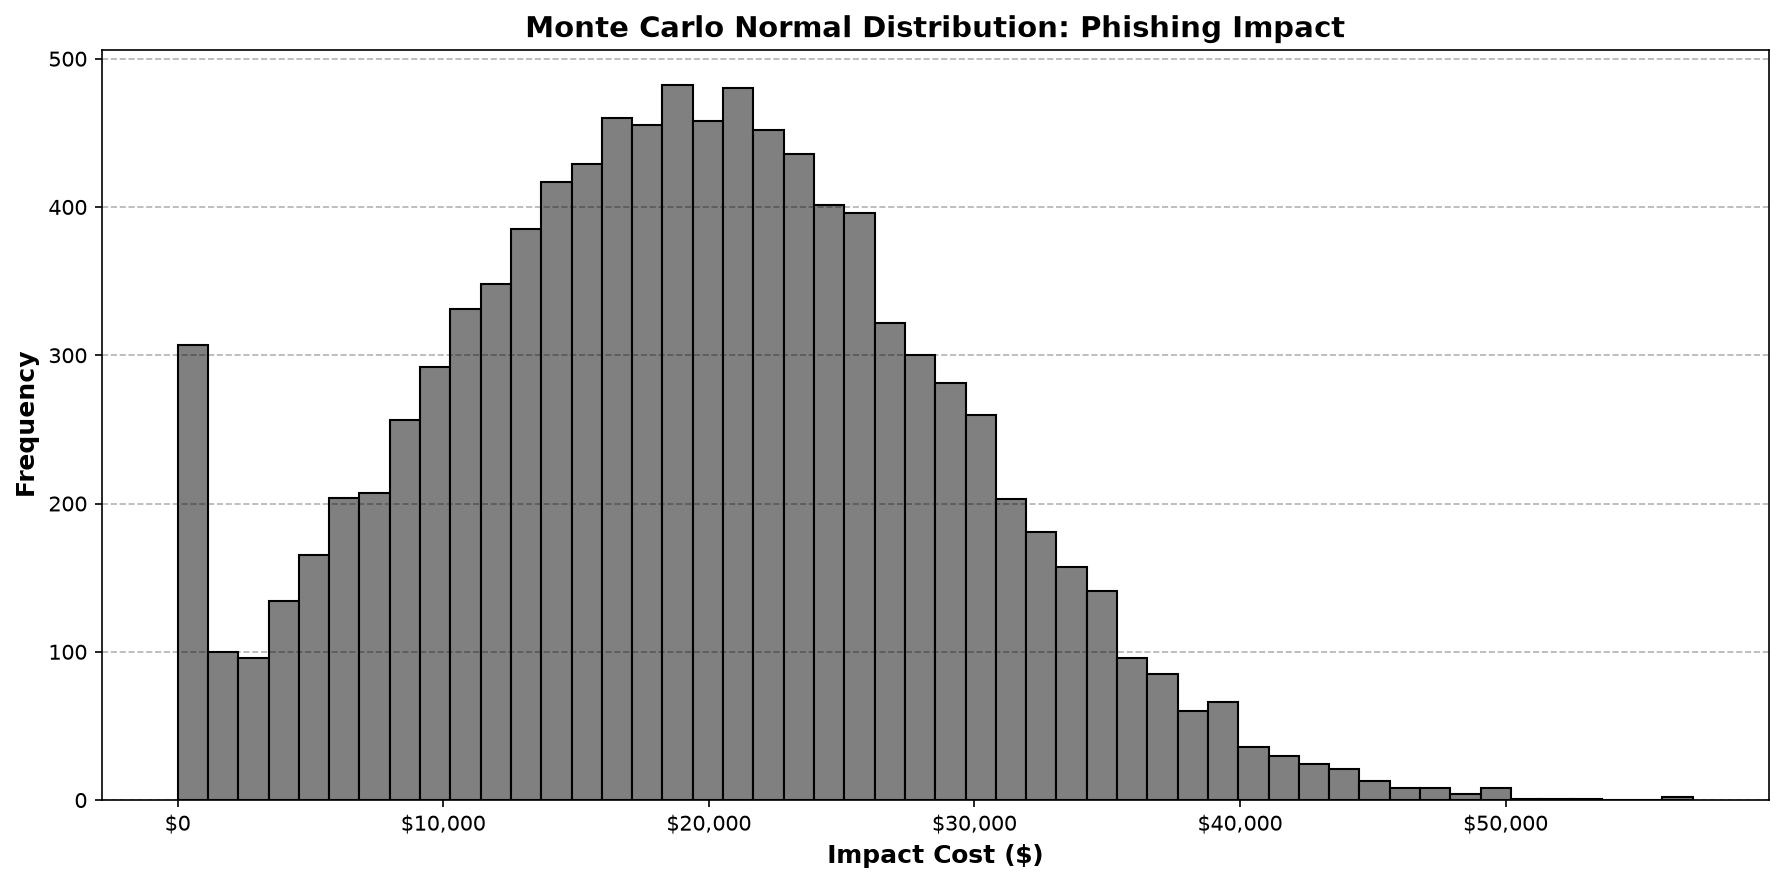
\includegraphics[width=\linewidth]{figures/histogram_phishing_impact.png}}}
  \caption{We ran a\index{Monte Carlo simulation} Monte Carlo simulation of 10,000 iterations with a normal distribution to spread random instances between bounds taken from means of seven year samples. We set a lower bound that the events would cost at \$0.  We set an upper bound that the events would cost \$46,695.  \protect\endnote{\index{sample} Sample size was set equivalent to the City of\index{Chattanooga} Chattanooga to determine the per capita rates for each year over data from \index{American Samoa} American Samoa and\index{California} California.  The medians of those rates were used to set upper and lower bounds with \index{American Samoa} American Samoa and\index{California} California representing low and high \index{cybercrime} \gls{cybercrime} counts respectively.}
  \protect\endnote{Monte Carlo Modeling Toolkit authored by Derek E. Brink, \gls{cissp}, \url{www.linkedin.com/in/derekbrink}. March 2023.}
  }
  \label{fig:screenshot-montecarlo-\gls{phishing}-impact-histo}
\end{figure}
\begin{figure}[H]
  \centering
  \rotatebox{0}{\scalebox{1}{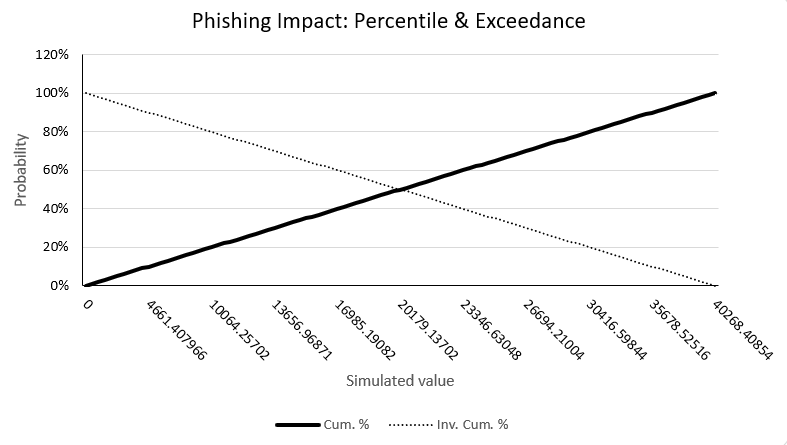
\includegraphics[width=\linewidth]{figures/percent_phishing_impact.png}}}
  \[
\mathrm{CI}_{80\%}(\theta) = [\$5081, \$41415]
\]
  
  \caption{A\index{Monte Carlo simulation} Monte Carlo simulation with a normal distribution suggests that there is a 90\% probability that\index{phishing} phishing events will cost \$4,418.61 or more in a year.  There is a 50\% likelihood that they will cost \$19,983.42 or more in a year.  There is a 10\% chance that they will cost \$35,551.27 or more in a year. \protect\endnote{\index{sample} sample size was set equivalent to the City of\index{Chattanooga} Chattanooga to determine the per capita rates for each year over data from \index{American Samoa} American Samoa and\index{California} California.  The medians of those rates were used to set 10\% and 90\%\index{confidence interval} confidence intervals with \index{American Samoa} American Samoa and\index{California} California representing low and high \index{cybercrime} cybercrime impact values respectively.}
  \protect\endnote{Monte Carlo Modeling Toolkit authored by Derek E. Brink, \gls{cissp}, \url{www.linkedin.com/in/derekbrink}. March 2023.}
  }
  \label{fig:screenshot-montecarlo-phishing-impact-percent}
\end{figure}
%%%%%%%%%%%%%%%%%%%%  RANSOMWARE\index{ransomware} %%%%%%%%%%%%%%%%%%%%%%%%
\newpage
\subsection{Ransomware}\label{sec:ransomware}
\subsubsection{Lower Bound Computation}
\[
\begin{bmatrix}
\mathbf{x}_{\text{American Samoa}}^{(\text{count})}\\
\mathbf{x}_{\text{American Samoa}}^{(\text{dollars})}
\end{bmatrix}
=
\begin{bmatrix}
0 & 0 & \cdots & 0\\
\$0 &\$0 & \cdots &\$0 
\end{bmatrix}.
\]
\[
\begin{bmatrix}
\mathbf{x}_{\text{American Samoa}}^{(\text{count scaled to sample population})}\\
\mathbf{x}_{\text{American Samoa}}^{(\text{dollars scaled to sample population})}
\end{bmatrix}
=
\begin{bmatrix}
0 & \cdots & 0\\
\$0 & \cdots &\$0
\end{bmatrix}.
\]
  \[
\bar{X}_{\text{American Samoa}}^{(m)}
= \frac{1}{N}\sum_{i=1}^{N} X_{\text{American Samoa},i}^{(m)},
\]
\\
\[
\qquad
m \in \{\text{scaled count},\text{scaled dollars}\}
\]
\[
\begin{bmatrix}
\bar{X}_{\text{American Samoa}}^{(\text{scaled count})}\\
\bar{X}_{\text{American Samoa}}^{(\text{scaled dollars})}
\end{bmatrix}
=
\begin{bmatrix}
0\\
\$0
\end{bmatrix}.
\]
\subsubsection{Upper Bound Computation}
\[
\begin{bmatrix}
\mathbf{x}_{\text{California}}^{(\text{count})}\\
\mathbf{x}_{\text{California}}^{(\text{dollars})}
\end{bmatrix}
=
\begin{bmatrix}
336 & 222 & \cdots & 296\\
\$260{,}331 &\$600{,}727  & \cdots &\$1{,}945{,}212 
\end{bmatrix}.
\]
\[
\begin{bmatrix}
\mathbf{x}_{\text{California}}^{(\text{count scaled to sample population})}\\
\mathbf{x}_{\text{California}}^{(\text{dollars scaled to sample population})}
\end{bmatrix}
=
\begin{bmatrix}
1 & 1 & \cdots & 1\\
\$775 &\$2{,}706 & \cdots &\$6{,}572 
\end{bmatrix}.
\]
\[
\bar{X}_{\text{California}}^{(m)}
= \frac{1}{N}\sum_{i=1}^{N} X_{\text{California},i}^{(m)},
\]
\\
\[
\qquad
m \in \{\text{scaled count},\text{scaled dollars}\}
\]
\[
\begin{bmatrix}
\bar{X}_{\text{California}}^{(\text{scaled count})}\\
\bar{X}_{\text{California}}^{(\text{scaled dollars})}
\end{bmatrix}
=
\begin{bmatrix}
1.06\\
\$6{,}761
\end{bmatrix}.
\]
\subsubsection{Monte Carlo Simulations for Likelihood and Impact}
\begin{figure}[H]
  \centering
  \rotatebox{0}{\scalebox{1}{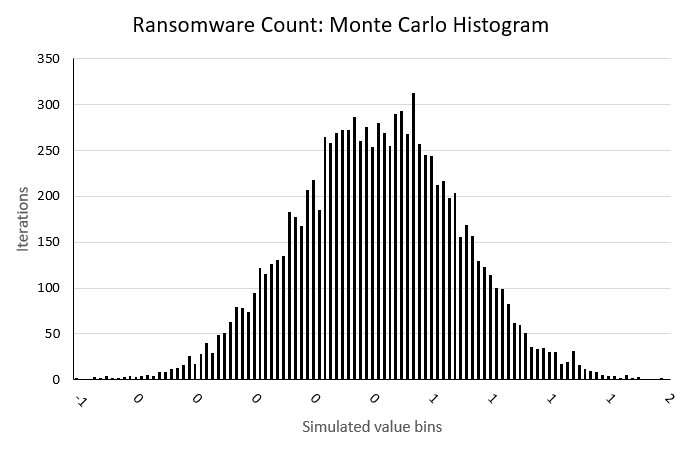
\includegraphics[width=\linewidth]{figures/histogram_ransomware.png}}}
  \caption{We ran a\index{Monte Carlo simulation} Monte Carlo simulation of 10,000 iterations to spread random instances between confidence intervals taken from means of a seven year sample. We bounded between 0 and 1 possible \gls{ransomware} events over a year.\protect\endnote{\index{sample} Sample size was set equivalent to the City of\index{Chattanooga} Chattanooga to determine the per capita rates for each year over data from \index{American Samoa} American Samoa and\index{California} California.  The medians of those rates were used to set upper and lower bounds with \index{American Samoa} American Samoa and\index{California} California representing low and high \index{cybercrime} \gls{cybercrime} counts respectively.}
  \protect\endnote{Monte Carlo Modeling Toolkit authored by Derek E. Brink, \gls{cissp}, \url{www.linkedin.com/in/derekbrink}. March 2023.}
  }
  \label{fig:screenshot-montecarlo-ransomware-count-histo}
\end{figure}

\begin{figure}[H]
  \centering
  \rotatebox{0}{\scalebox{1}{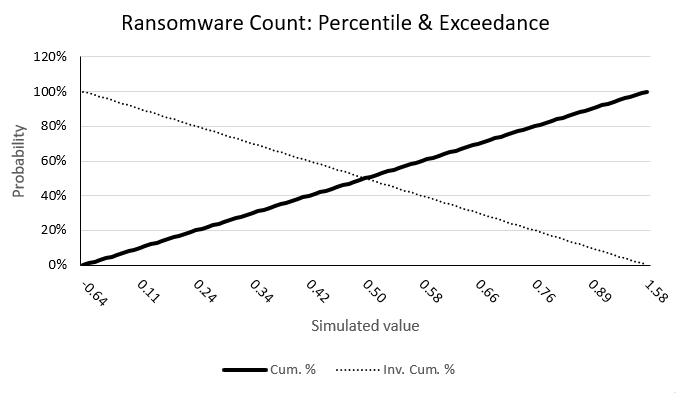
\includegraphics[width=\linewidth]{figures/count_ransomware_percentile.png}}}
  \caption{A\index{Monte Carlo simulation} Monte Carlo simulation suggests that there is a 50\% probability that 0.5 or more\index{ransomware} ransomware events will occur within the \index{sample} sample.  This unusual result is because the confidence bounds are between 0 and 1.  We interpret this as a 50\% probability that one malware event will occur. \protect\endnote{\index{sample} Sample size was set equivalent to the City of\index{Chattanooga} Chattanooga to determine the per capita rates for each year over data from \index{American Samoa} American Samoa and\index{California} California.  The medians of those rates were used to set upper and lower bounds with \index{American Samoa} American Samoa and\index{California} California representing low and high \index{cybercrime} cybercrime counts respectively.}
  \protect\endnote{Monte Carlo Modeling Toolkit authored by Derek E. Brink, \gls{cissp}, \url{www.linkedin.com/in/derekbrink}. March 2023.}
  }
  \label{fig:screenshot-montecarlo-\gls{ransomware}-count-percent}
\end{figure}

\begin{figure}[H]
  \centering
  \rotatebox{0}{\scalebox{1}{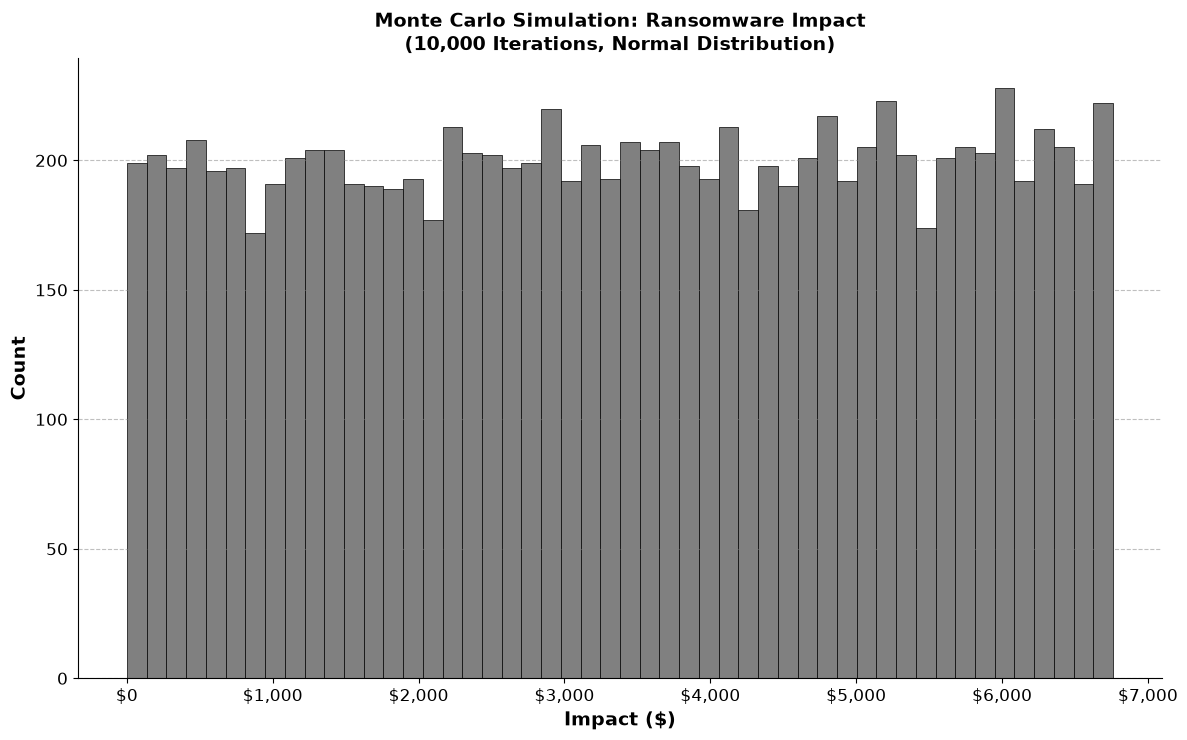
\includegraphics[width=\linewidth]{figures/histogram_ransomware_impact.png}}}
  \caption{We ran a\index{Monte Carlo simulation} Monte Carlo simulation of 10,000 iterations to spread random instances between confidence intervals taken from means of a seven year sample. We set a lower bound that the event would cost at \$0.  We set an upper bound that the event would cost \$3,479.\protect\endnote{\index{sample} Sample size was set equivalent to the City of\index{Chattanooga} Chattanooga to determine the per capita rates for each year over data from \index{American Samoa} American Samoa and\index{California} California.  The medians of those rates were used to set upper and lower bounds with \index{American Samoa} American Samoa and\index{California} California representing low and high \index{cybercrime} \gls{cybercrime} counts respectively.}
  \protect\endnote{Monte Carlo Modeling Toolkit authored by Derek E. Brink, \gls{cissp}, \url{www.linkedin.com/in/derekbrink}. March 2023.}
  }
  \label{fig:screenshot-montecarlo-\gls{ransomware}-impact-histo}
\end{figure}

\begin{figure}[H]
  \centering
  \rotatebox{0}{\scalebox{1}{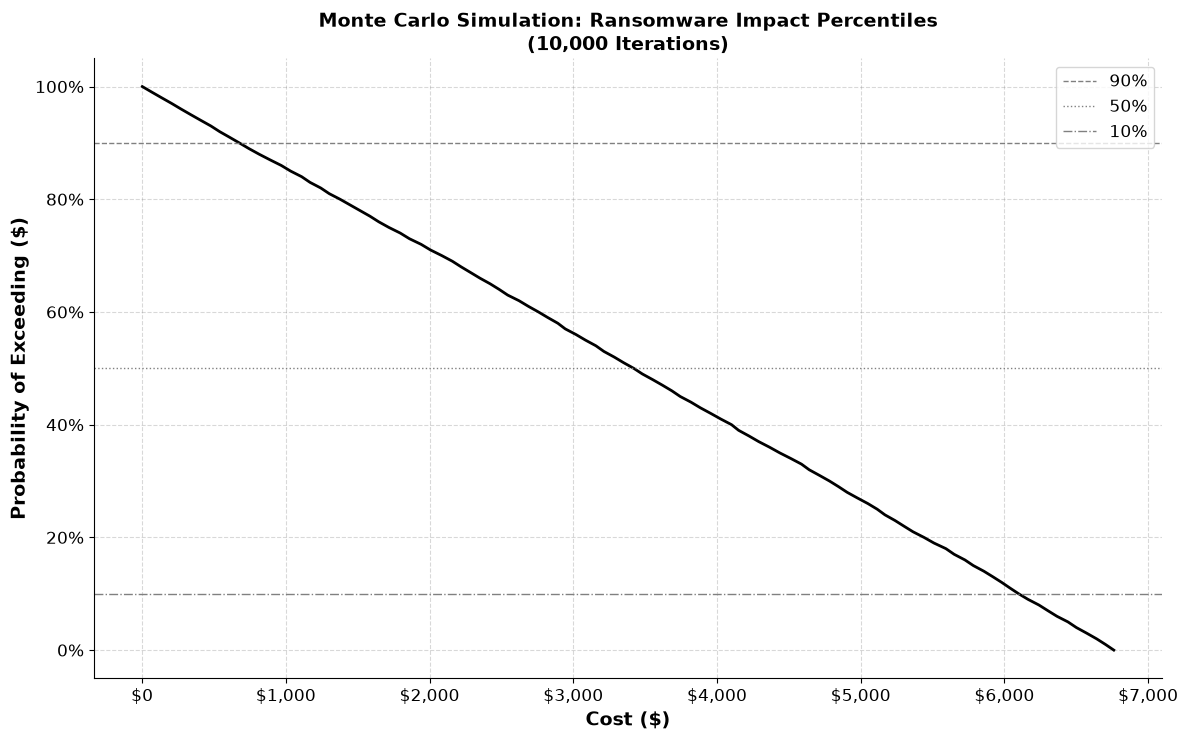
\includegraphics[width=\linewidth]{figures/percent_ransomware_impact.png}}}
  \caption{A\index{Monte Carlo simulation} Monte Carlo simulation suggests that there is a 90\% probability that\index{ransomware} ransomware events will cost \$394.39 or more in a year.  There is a 50\% likelihood that they will cost \$1,754.94 or more in a year.  There is a 10\% chance that they will cost \$3,111.30 or more in a year. \protect\endnote{\index{sample} sample size was set equivalent to the City of\index{Chattanooga} Chattanooga to determine the per capita rates for each year over data from \index{American Samoa} American Samoa and\index{California} California.  The medians of those rates were used to set 10\% and 90\%\index{confidence interval} confidence intervals with \index{American Samoa} American Samoa and\index{California} California representing low and high \index{cybercrime} cybercrime impact values respectively.}
  \protect\endnote{Monte Carlo Modeling Toolkit authored by Derek E. Brink, \gls{cissp}, \url{www.linkedin.com/in/derekbrink}. March 2023.}
  }
  \label{fig:screenshot-montecarlo-ransomware-impact-percent}
\end{figure}
\FloatBarrier
\subsection{Threats to Personnel}
\begin{table}[H]
  \centering
  \caption{Projected In-City Victim Counts, City of\index{Chattanooga} Chattanooga, Threats to Personnel}
  \label{tab:chattanoogacrime4}
  \begin{center}
  \begin{tabular}{@{}>{\centering\arraybackslash}
  p{0.05\linewidth} >{\centering\arraybackslash}
  p{0.25\linewidth} >{\centering\arraybackslash}
  p{0.25\linewidth} >{\centering\arraybackslash}
  p{0.25\linewidth} >{\centering\arraybackslash}
  p{0.05\linewidth}}
    \toprule
    Year &
    \rotatebox{90}{\begin{tabular}{@{}ll@{}}Crimes Against\\Children\end{tabular}} &
    \rotatebox{90}{\begin{tabular}{@{}ll@{}}Extortion\end{tabular}} &
    \rotatebox{90}{\begin{tabular}{@{}ll@{}}Threats, Stalking,\\Harassment, and Terrorism\end{tabular}} &
 \\
\midrule
2016&0&9&7&\endnote{original\protect\url{https://www.ic3.gov/Media/PDF/AnnualReport/2016State/StateReport.aspx\#?s=47} current \protect\url{https://www.ic3.gov/AnnualReport/Reports/2016_IC3Report.pdf}}\\
2017&0&7&6&\endnote{original:\protect\url{https://www.ic3.gov/Media/PDF/AnnualReport/2017State/StateReport.aspx\#?s=47} current: \url{https://www.ic3.gov/AnnualReport/Reports/2017_IC3Report.pdf}}\\
2018&0&20&7&\endnote{original:\protect\url{https://www.ic3.gov/Media/PDF/AnnualReport/2018State/StateReport.aspx\#?s=47} current: \url{https://www.ic3.gov/AnnualReport/Reports/2018_IC3Report.pdf}}\\
2019&0&19&5&\endnote{original:\protect\url{https://www.ic3.gov/Media/PDF/AnnualReport/2019State/StateReport.aspx\#?s=47} current: \url{https://www.ic3.gov/AnnualReport/Reports/2019_IC3Report.pdf}}\\
2020&1&31&6&\endnote{original:\protect\url{https://www.ic3.gov/Media/PDF/AnnualReport/2020State/StateReport.aspx\#?s=47} current: \url{https://www.ic3.gov/AnnualReport/Reports/2020_IC3Report.pdf}}\\
2021&0&0&4&\endnote{original:\protect\url{https://www.ic3.gov/Media/PDF/AnnualReport/2021State/StateReport.aspx\#?s=47} current: \url{https://www.ic3.gov/AnnualReport/Reports/2021_IC3Report.pdf}}\\
2022&1&18&0&\endnote{original:\protect\url{https://www.ic3.gov/Media/PDF/AnnualReport/2022State/StateReport.aspx\#?s=47} current: \url{https://www.ic3.gov/AnnualReport/Reports/2022_IC3Report.pdf}}\\

    \bottomrule 
    \end{tabular}
    \end{center}
  \raggedright{Counts deduced from \gls{ic3} Victim Complaints for Tennessee adjusted for a per-capita rate and then multiplied by the city's \index{population} population for that year.  Threats, stalking, and harrassment counts were combined with terrorism because the mechanisms were similar.}
\end{table}
%%%%%%%%%%%%%%% CRIMES AGAINST CHILDREN %%%%%%%%%%%%%%%%%%%
\newpage
\subsection{Crimes Against Children}
\subsubsection{Lower Bound Computation}
\[
\begin{bmatrix}
\mathbf{x}_{\text{American Samoa}}^{(\text{count})}\\
\mathbf{x}_{\text{American Samoa}}^{(\text{dollars})}
\end{bmatrix}
=
\begin{bmatrix}
0 & 0 & \cdots & 3\\
\$0 &\$0 & \cdots &\$11 
\end{bmatrix}.
\]
% Columns represent years 2016, \cdots, 2017, \cdots, 2022 for American Samoa Crimes Against Children.
% Raw counts: 2016=0, 2017=0, 2022=3.  Raw dollars: 2016=\$0, 2017=\$0, 2022=\$11.
\[
\begin{bmatrix}
\mathbf{x}_{\text{American Samoa}}^{(\text{count scaled to sample population})}\\
\mathbf{x}_{\text{American Samoa}}^{(\text{dollars scaled to sample population})}
\end{bmatrix}
=
\begin{bmatrix}
0 & \cdots & 11.42\\
\$0 & \cdots &\$41.89
\end{bmatrix}.
\]
% Per-capita scaled to Chattanooga population:
% 2016=0, 2017=0, 2022=11.42 victims; dollars: 2016=\$0, 2017=\$0, 2022=\$41.89.
  \[
\bar{X}_{\text{American Samoa}}^{(m)}
= \frac{1}{N}\sum_{i=1}^{N} X_{\text{American Samoa},i}^{(m)},
\]
\\
\[
\qquad
m \in \{\text{scaled count},\text{scaled dollars}\}
\]
\[
\begin{bmatrix}
\bar{X}_{\text{American Samoa}}^{(\text{scaled count})}\\
\bar{X}_{\text{American Samoa}}^{(\text{scaled dollars})}
\end{bmatrix}
=
\begin{bmatrix}
1.63\\
\$5.98
\end{bmatrix}.
\]
\subsubsection{Upper Bound Computation}
\[
\begin{bmatrix}
\mathbf{x}_{\text{California}}^{(\text{count})}\\
\mathbf{x}_{\text{California}}^{(\text{dollars})}
\end{bmatrix}
=
\begin{bmatrix}
142 & 125 & \cdots & 256\\
\$2{,}764 &\$1{,}050  & \cdots &\$1 
\end{bmatrix}.
\]
% Raw California counts: 2016=142, 2017=125, 2022=256.
% Raw California dollars: 2016=\$2,764, 2017=\$1,050, 2022=\$1.
\[
\begin{bmatrix}
\mathbf{x}_{\text{California}}^{(\text{count scaled to sample population})}\\
\mathbf{x}_{\text{California}}^{(\text{dollars scaled to sample population})}
\end{bmatrix}
=
\begin{bmatrix}
0.64 & 0.57 & \cdots & 1.20\\
\$12.55 &\$4.79 & \cdots &\$0.00
\end{bmatrix}.
\]
% California scaled to Chattanooga: 2016=0.64, 2017=0.57, 2022=1.20.
% Scaled dollars: 2016=\$12.55, 2017=\$4.79, 2022=\$0.00.
\[
\bar{X}_{\text{California}}^{(m)}
= \frac{1}{N}\sum_{i=1}^{N} X_{\text{California},i}^{(m)},
\]
\\
\[
\qquad
m \in \{\text{scaled count},\text{scaled dollars}\}
\]
\[
\begin{bmatrix}
\bar{X}_{\text{California}}^{(\text{scaled count})}\\
\bar{X}_{\text{California}}^{(\text{scaled dollars})}
\end{bmatrix}
=
\begin{bmatrix}
0.98\\
\$299.93
\end{bmatrix}.
\]
\subsubsection{Monte Carlo Simulations for Likelihood and Impact}
\begin{figure}[H]
  \centering
  \rotatebox{0}{\scalebox{1}{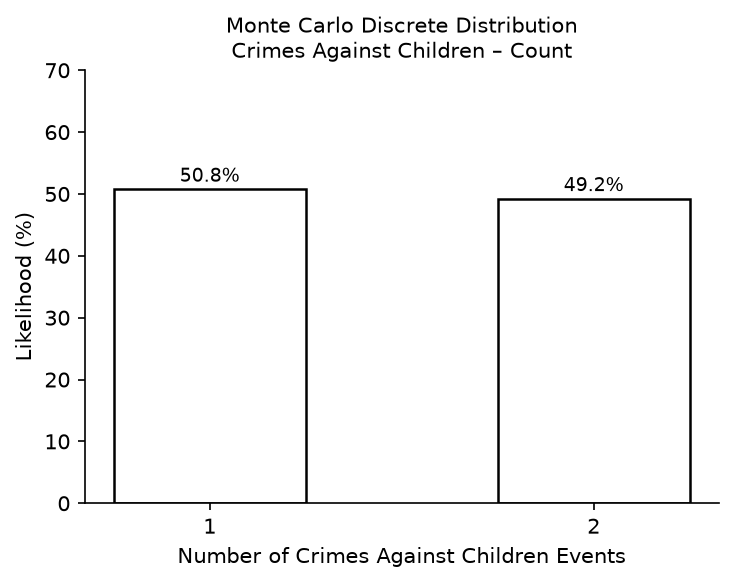
\includegraphics[width=\linewidth]{figures/discrete_children_count.png}}}
  \caption{We ran a\index{Monte Carlo simulation} Monte Carlo simulation of 10,000 iterations with a discrete distribution to spread random instances between upper and lower bounds taken from the means of seven year samples. We bounded between 1 and 2 possible \index{crimes against children}crimes against children events over a year.\protect\endnote{\index{sample} Sample size was set equivalent to the City of\index{Chattanooga} Chattanooga to determine the per capita rates for each year over data from \index{American Samoa} American Samoa and\index{California} California.  The means of those rates were used to set upper and lower bounds with \index{American Samoa} American Samoa and\index{California} California representing low and high \index{cybercrime} \gls{cybercrime} counts respectively.}
  \protect\endnote{Monte Carlo Modeling Toolkit authored by Derek E. Brink, \gls{cissp}, \url{www.linkedin.com/in/derekbrink}. March 2023.}
  }
  \label{fig:screenshot-montecarlo-children-count-discrete}
\end{figure}
When we computed the upper and lower bounds, we recognized that a normal distribution would not fit well for forecasting likelihood.  We took the mean of the sample from American Samoa for the lower bound (2); we took the mean from the sample from California for the upper bound (1); we had a separation of 1 unit.  Therefore, we switched to a discrete model with all 2 options sharing an equal likelihood.
\begin{table}[H]
  \centering
  \caption{Monte Carlo Discrete Simulation Values for Crimes Against Children}
  \label{tab:discrete_children_montecarlo}
  \begin{center}
  \begin{tabular}{@{}>{\centering\arraybackslash}
  p{0.30\linewidth} >{\centering\arraybackslash}
  p{0.20\linewidth} >{\centering\arraybackslash}
  p{0.20\linewidth}}
    \toprule
Events
&1
&2\\
    \midrule
Likelihood    
&50.8\%
&49.2\%\\
    \bottomrule \end{tabular}
    \end{center}
  \raggedright{A\index{Monte Carlo simulation} Monte Carlo simulation was run using a discrete distribution.  We bounded the simulation between 1 and 2 events.  We assigned a 50\% likelihood to each bin.  The resulting distribution showed the effect of randomness on each possible outcome.}
\end{table}

\begin{figure}[H]
  \centering
  \rotatebox{0}{\scalebox{1}{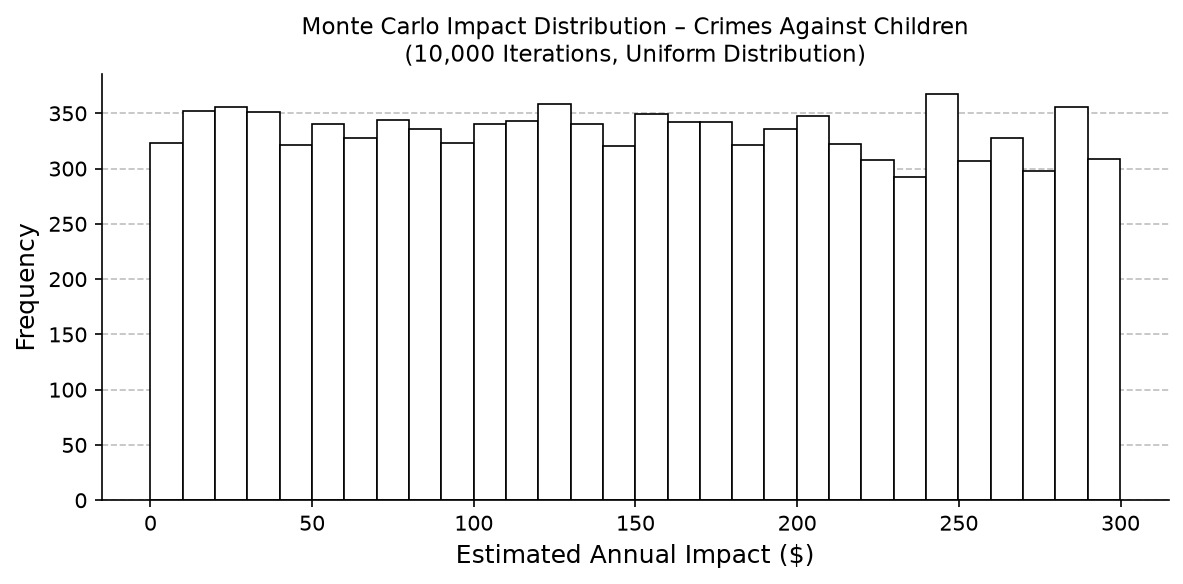
\includegraphics[width=\linewidth]{figures/histogram_children_impact.png}}}
  \caption{We ran a\index{Monte Carlo simulation} Monte Carlo simulation of 10,000 iterations with a normal distribution to spread random instances between bounds taken from means of seven year samples. We set a lower bound that the events would cost at \$0.  We set an upper bound that the events would cost \$299.93.  \protect\endnote{\index{sample} Sample size was set equivalent to the City of\index{Chattanooga} Chattanooga to determine the per capita rates for each year over data from \index{American Samoa} American Samoa and\index{California} California.  The means of those rates were used to set upper and lower bounds with \index{American Samoa} American Samoa and\index{California} California representing low and high \index{cybercrime} \gls{cybercrime} counts respectively.}
  \protect\endnote{Monte Carlo Modeling Toolkit authored by Derek E. Brink, \gls{cissp}, \url{www.linkedin.com/in/derekbrink}. March 2023.}
  }
  \label{fig:screenshot-montecarlo-children-impact-histo}
\end{figure}
\begin{figure}[H]
  \centering
  \rotatebox{0}{\scalebox{1}{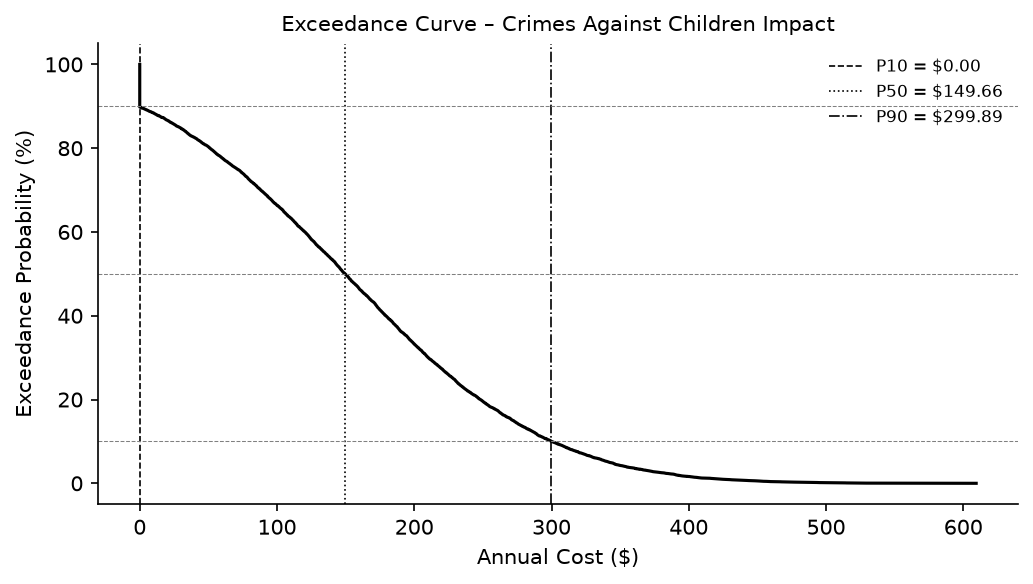
\includegraphics[width=\linewidth]{figures/percent_children_impact.png}}}
  \[
\mathrm{CI}_{80\%}(\theta) = [\$0, \$299.89]
\]
  \caption{A\index{Monte Carlo simulation} Monte Carlo simulation with a normal distribution suggests that there is a 90\% probability that\index{crimes against children} crimes against children events will cost \$0.00 or more in a year.  There is a 50\% likelihood that they will cost \$149.66 or more in a year.  There is a 10\% chance that they will cost \$299.89 or more in a year. \protect\endnote{\index{sample} sample size was set equivalent to the City of\index{Chattanooga} Chattanooga to determine the per capita rates for each year over data from \index{American Samoa} American Samoa and\index{California} California.  The means of those rates were used to set 10\% and 90\%\index{confidence interval} confidence intervals with \index{American Samoa} American Samoa and\index{California} California representing low and high \index{cybercrime} cybercrime impact values respectively.}
  \protect\endnote{Monte Carlo Modeling Toolkit authored by Derek E. Brink, \gls{cissp}, \url{www.linkedin.com/in/derekbrink}. March 2023.}
  }
  \label{fig:screenshot-montecarlo-children-impact-percent}
\end{figure}
%%%%%%%%%%%%%%%%%%%%  EXTORTION %%%%%%%%%%%%%%%%%%%%%%%%
\newpage
\subsection{Extortion}\label{sec:extortion}
\subsubsection{Lower Bound Computation}
\[
\begin{bmatrix}
\mathbf{x}_{\text{American Samoa}}^{(\text{count})}\\
\mathbf{x}_{\text{American Samoa}}^{(\text{dollars})}
\end{bmatrix}
=
\begin{bmatrix}
2 & 1 & \cdots & 2\\
\$0 & \$0 & \cdots & \$7
\end{bmatrix}.
\]
\[
\begin{bmatrix}
\mathbf{x}_{\text{American Samoa}}^{(\text{count scaled to sample population})}\\
\mathbf{x}_{\text{American Samoa}}^{(\text{dollars scaled to sample population})}
\end{bmatrix}
=
\begin{bmatrix}
6 & \cdots & 7.62\\
\$0 & \cdots & \$300
\end{bmatrix}.
\]
  \[
\bar{X}_{\text{American Samoa}}^{(m)}
= \frac{1}{N}\sum_{i=1}^{N} X_{\text{American Samoa},i}^{(m)},
\]
\\
\[
\qquad
m \in \{\text{scaled count},\text{scaled dollars}\}
\]
\[
\begin{bmatrix}
\bar{X}_{\text{American Samoa}}^{(\text{scaled count})}\\
\bar{X}_{\text{American Samoa}}^{(\text{scaled dollars})}
\end{bmatrix}
=
\begin{bmatrix}
5.60\\
\$300
\end{bmatrix}.
\]
\subsubsection{Upper Bound Computation}
\[
\begin{bmatrix}
\mathbf{x}_{\text{California}}^{(\text{count})}\\
\mathbf{x}_{\text{California}}^{(\text{dollars})}
\end{bmatrix}
=
\begin{bmatrix}
2{,}257 & 2{,}054 & \cdots & 4{,}746\\
\$2{,}413{,}243 & \$1{,}725{,}544 & \cdots & \$22
\end{bmatrix}.
\]
\[
\begin{bmatrix}
\mathbf{x}_{\text{California}}^{(\text{count scaled to sample population})}\\
\mathbf{x}_{\text{California}}^{(\text{dollars scaled to sample population})}
\end{bmatrix}
=
\begin{bmatrix}
10 & 9 & \cdots & 22.33\\
\$10{,}692.26 & \$7{,}560.81 & \cdots & \$2{,}331.31
\end{bmatrix}.
\]
\[
\bar{X}_{\text{California}}^{(m)}
= \frac{1}{N}\sum_{i=1}^{N} X_{\text{California},i}^{(m)},
\]
\\
\[
\qquad
m \in \{\text{scaled count},\text{scaled dollars}\}
\]
\[
\begin{bmatrix}
\bar{X}_{\text{California}}^{(\text{scaled count})}\\
\bar{X}_{\text{California}}^{(\text{scaled dollars})}
\end{bmatrix}
=
\begin{bmatrix}
26.48\\
\$43{,}167.06
\end{bmatrix}.
\]
\subsubsection{Monte Carlo Simulations for Likelihood and Impact}
\begin{figure}[H]
  \centering
  \rotatebox{0}{\scalebox{1}{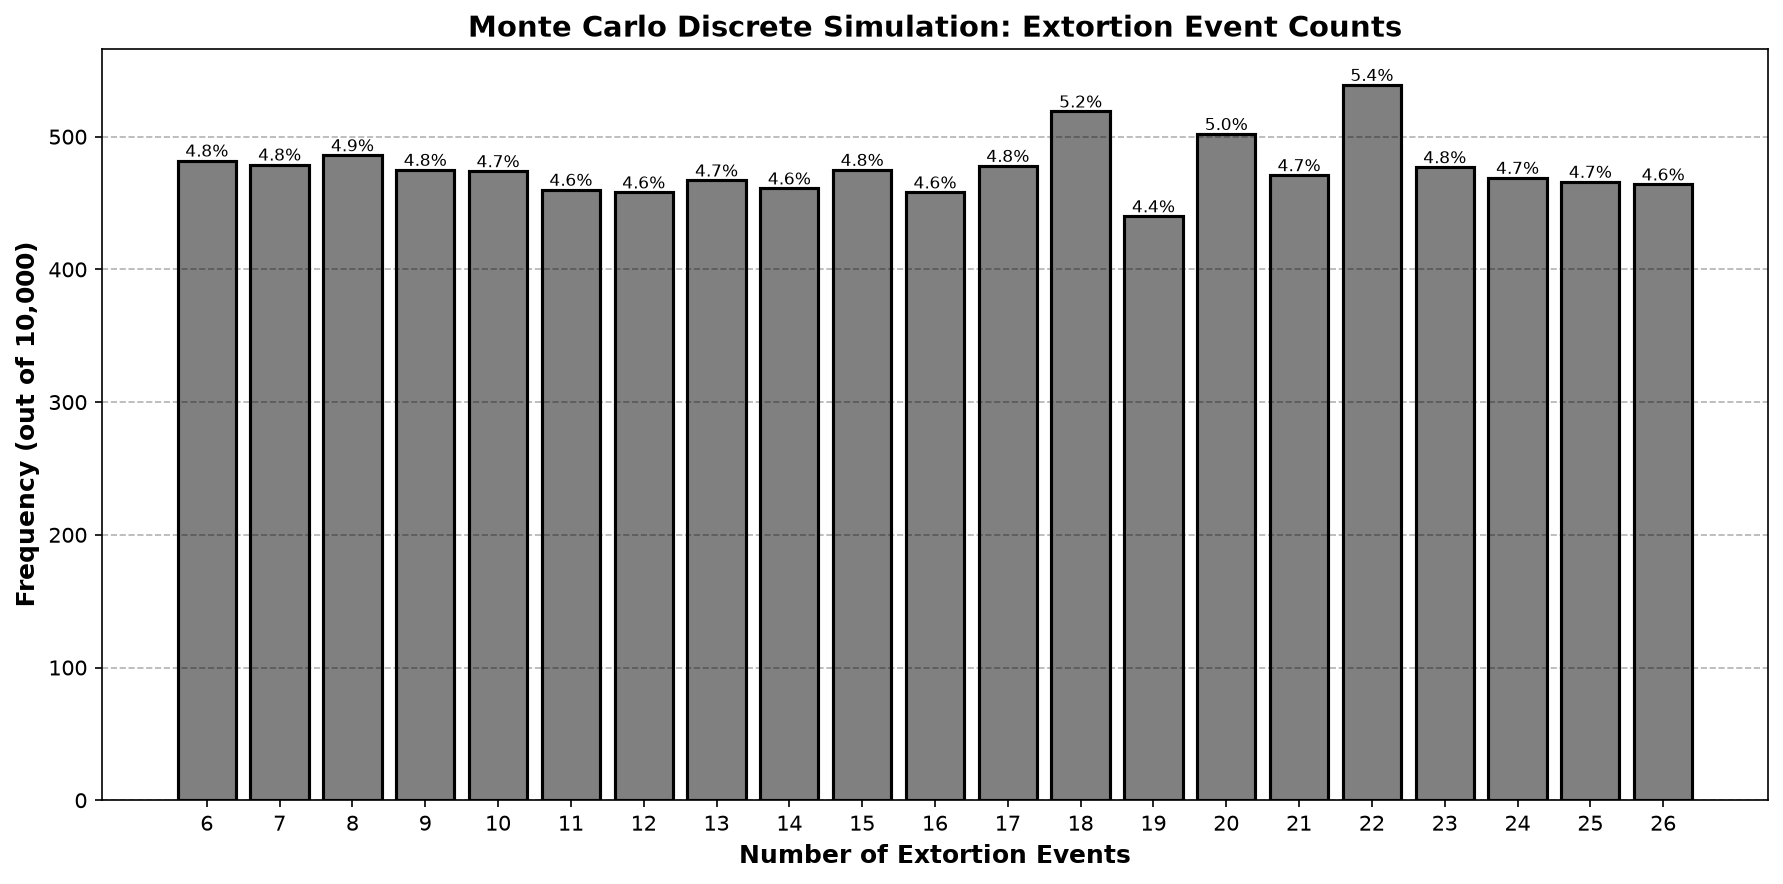
\includegraphics[width=\linewidth]{figures/discrete_extortion_count.png}}}
  \caption{We ran a\index{Monte Carlo simulation} Monte Carlo simulation of 10,000 iterations with a discrete distribution to spread random instances between upper and lower bounds taken from the means of seven year samples. We bounded between 6 and 26 possible \index{extortion}extortion events over a year.\protect\endnote{\index{sample} Sample size was set equivalent to the City of\index{Chattanooga} Chattanooga to determine the per capita rates for each year over data from \index{American Samoa} American Samoa and\index{California} California.  The means of those rates were used to set upper and lower bounds with \index{American Samoa} American Samoa and\index{California} California representing low and high \index{cybercrime} cybercrime counts respectively.}
  \protect\endnote{Monte Carlo Modeling Toolkit authored by Derek E. Brink, CISSP, \url{www.linkedin.com/in/derekbrink}. March 2023.}
  }
  \label{fig:screenshot-montecarlo-extortion-count-discrete}
\end{figure}
When we computed the upper and lower bounds, we recognized that a normal distribution would not fit well for forecasting likelihood.  We took the mean of the sample from American Samoa for the lower bound (5.60, rounded to 6); we took the mean from the sample from California for the upper bound (26.48, rounded to 26); we had a separation of 20 units.  Therefore, we switched to a discrete model with all 21 options sharing an equal likelihood.
\begin{table}[H]
  \centering
  \caption{Monte Carlo Discrete Simulation Values for Extortion}
  \label{tab:discrete_extortion_montecarlo}
  \begin{center}
  \begin{tabular}{@{}>{\centering\arraybackslash}
  p{0.20\linewidth} >{\centering\arraybackslash}
  p{0.10\linewidth} >{\centering\arraybackslash}
  p{0.10\linewidth} >{\centering\arraybackslash}
  p{0.10\linewidth} >{\centering\arraybackslash}
  p{0.10\linewidth} >{\centering\arraybackslash}
  p{0.10\linewidth}}
    \toprule
Events
    &6
    &7
    &8
    &9
    &10\\
    \midrule
Likelihood
    &4.8\%
    &4.8\%
    &4.8\%
    &4.8\%
    &4.8\%\\
    \bottomrule \end{tabular}
  \begin{tabular}{@{}>{\centering\arraybackslash}
  p{0.20\linewidth} >{\centering\arraybackslash}
  p{0.10\linewidth} >{\centering\arraybackslash}
  p{0.10\linewidth} >{\centering\arraybackslash}
  p{0.10\linewidth} >{\centering\arraybackslash}
  p{0.10\linewidth} >{\centering\arraybackslash}
  p{0.10\linewidth}}
    \toprule
Events
    &11
    &12
    &13
    &14
    &15\\
    \midrule
Likelihood
    &4.8\%
    &4.8\%
    &4.8\%
    &4.8\%
    &4.8\%\\
    \bottomrule \end{tabular}
  \begin{tabular}{@{}>{\centering\arraybackslash}
  p{0.20\linewidth} >{\centering\arraybackslash}
  p{0.10\linewidth} >{\centering\arraybackslash}
  p{0.10\linewidth} >{\centering\arraybackslash}
  p{0.10\linewidth} >{\centering\arraybackslash}
  p{0.10\linewidth} >{\centering\arraybackslash}
  p{0.10\linewidth}}
    \toprule
Events
    &16
    &17
    &18
    &19
    &20\\
    \midrule
Likelihood
    &4.8\%
    &4.8\%
    &4.8\%
    &4.8\%
    &4.8\%\\
    \bottomrule \end{tabular}
  \begin{tabular}{@{}>{\centering\arraybackslash}
  p{0.20\linewidth} >{\centering\arraybackslash}
  p{0.10\linewidth} >{\centering\arraybackslash}
  p{0.10\linewidth} >{\centering\arraybackslash}
  p{0.10\linewidth} >{\centering\arraybackslash}
  p{0.10\linewidth} >{\centering\arraybackslash}
  p{0.10\linewidth}}
    \toprule
Events
    &21
    &22
    &23
    &24
    &25\\
    \midrule
Likelihood
    &4.8\%
    &4.8\%
    &4.8\%
    &4.8\%
    &4.8\%\\
    \bottomrule \end{tabular}
  \begin{tabular}{@{}>{\centering\arraybackslash}
  p{0.20\linewidth} >{\centering\arraybackslash}
  p{0.10\linewidth}}
    \toprule
Events
    &26\\
    \midrule
Likelihood
    &4.8\%\\
    \bottomrule \end{tabular}
    \end{center}
  \raggedright{A\index{Monte Carlo simulation} Monte Carlo simulation was run using a discrete distribution.  We bounded the simulation between 6 and 26 events.  We assigned an approximately 4.8\% likelihood to each bin.  The resulting distribution showed the effect of randomness on each possible outcome.}
\end{table}

\begin{figure}[H]
  \centering
  \rotatebox{0}{\scalebox{1}{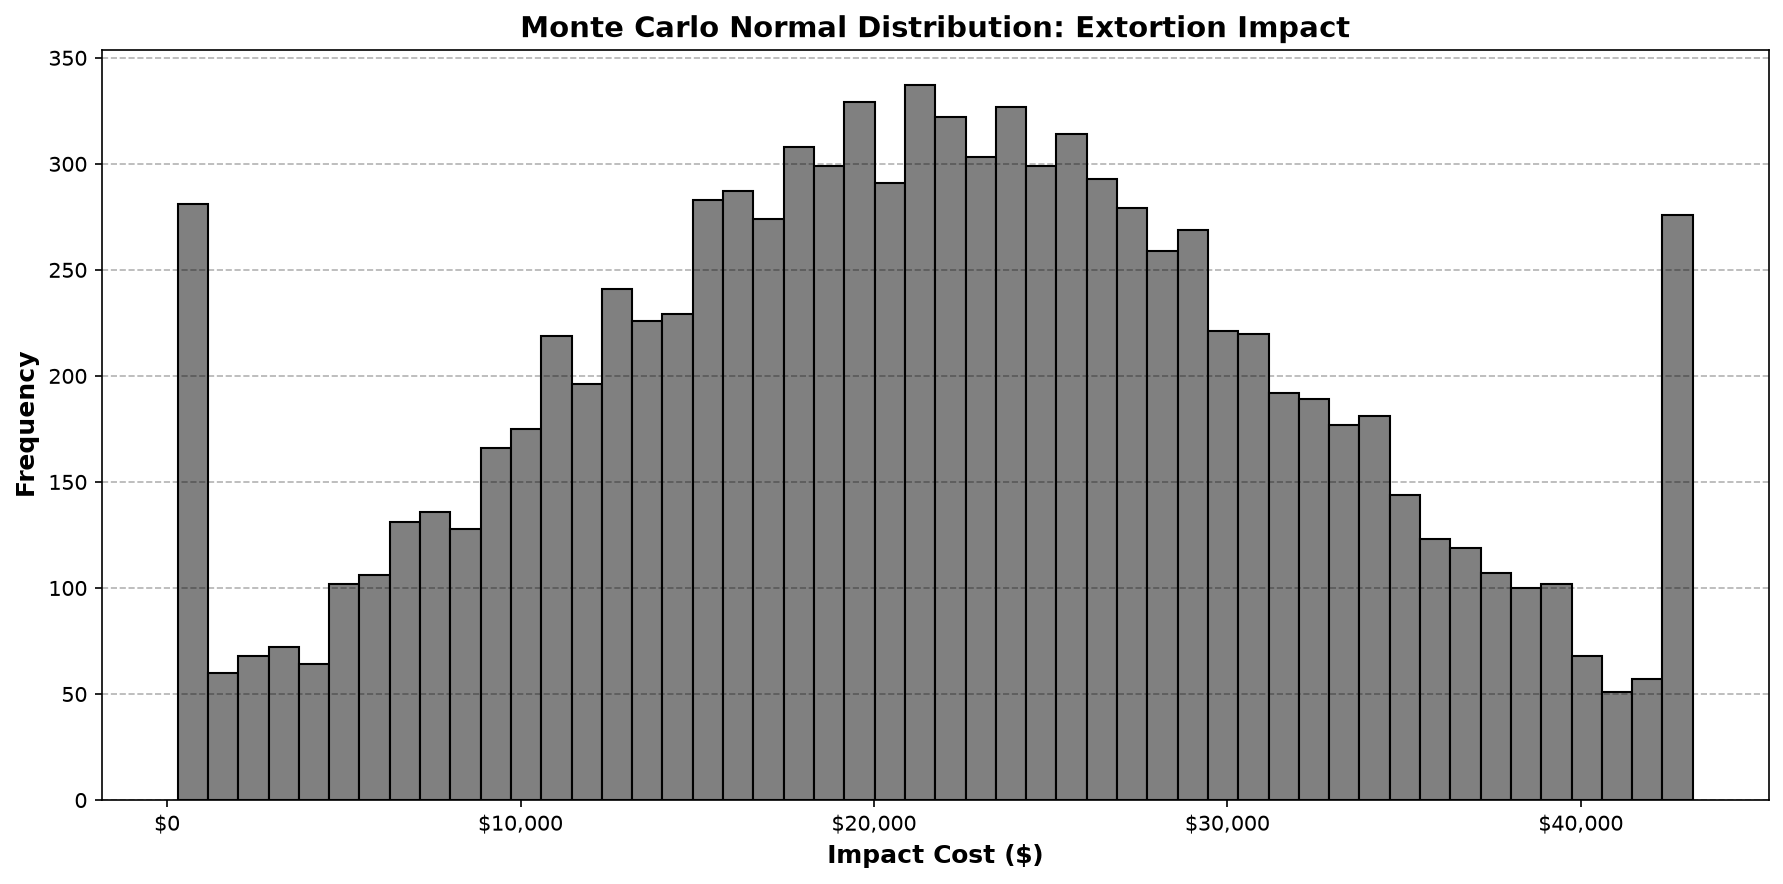
\includegraphics[width=\linewidth]{figures/histogram_extortion_impact.png}}}
  \caption{We ran a\index{Monte Carlo simulation} Monte Carlo simulation of 10,000 iterations with a normal distribution to spread random instances between bounds taken from means of seven year samples. We set a lower bound that the events would cost at \$300.  We set an upper bound that the events would cost \$43{,}167.06.  \protect\endnote{\index{sample} Sample size was set equivalent to the City of\index{Chattanooga} Chattanooga to determine the per capita rates for each year over data from \index{American Samoa} American Samoa and\index{California} California.  The means of those rates were used to set upper and lower bounds with \index{American Samoa} American Samoa and\index{California} California representing low and high \index{extortion} extortion impact values respectively.}
  \protect\endnote{Monte Carlo Modeling Toolkit authored by Derek E. Brink, CISSP, \url{www.linkedin.com/in/derekbrink}. March 2023.}
  }
  \label{fig:screenshot-montecarlo-extortion-impact-histo}
\end{figure}
\begin{figure}[H]
  \centering
  \rotatebox{0}{\scalebox{1}{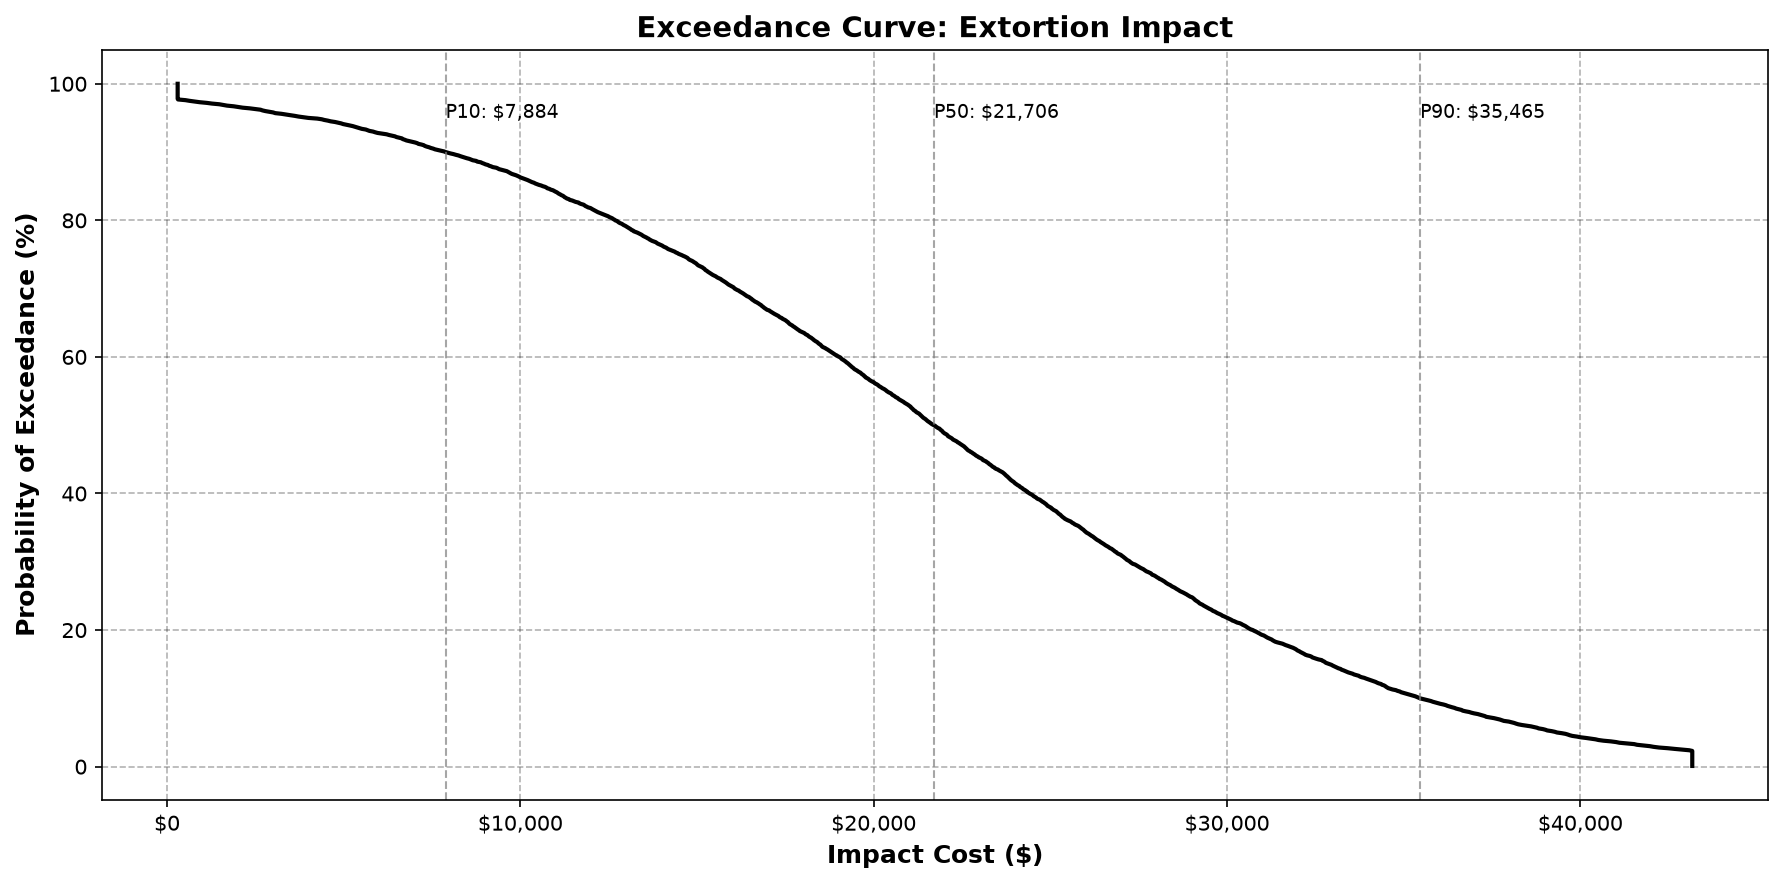
\includegraphics[width=\linewidth]{figures/percent_extortion_impact.png}}}
  \[
\mathrm{CI}_{80\%}(\theta) = [\${P10}, \${P90}]
\]
  \caption{A\index{Monte Carlo simulation} Monte Carlo simulation with a normal distribution suggests that there is a 90\% probability that\index{extortion} extortion events will cost \${P10} or more in a year.  There is a 50\% likelihood that they will cost \${P50} or more in a year.  There is a 10\% chance that they will cost \${P90} or more in a year. \protect\endnote{\index{sample} sample size was set equivalent to the City of\index{Chattanooga} Chattanooga to determine the per capita rates for each year over data from \index{American Samoa} American Samoa and\index{California} California.  The means of those rates were used to set upper and lower bounds with \index{American Samoa} American Samoa and\index{California} California representing low and high \index{extortion} extortion impact values respectively.}
  \protect\endnote{Monte Carlo Modeling Toolkit authored by Derek E. Brink, CISSP, \url{www.linkedin.com/in/derekbrink}. March 2023.}
  }
  \label{fig:screenshot-montecarlo-extortion-impact-percent}
\end{figure}

%%%%%%%%%%% THREATS, STALKING, HARASSMENT, TERRORISM %%%%%%%%%%
\subsection{Threats, Stalking, Harassment, and Terrorism}
\subsubsection{Lower Bound Computation}
\[
\begin{bmatrix}
\mathbf{x}_{\text{American Samoa}}^{(\text{count})}\\
\mathbf{x}_{\text{American Samoa}}^{(\text{dollars})}
\end{bmatrix}
=
\begin{bmatrix}
3 & 3 & \cdots & 1\\
\$0 &\$0 & \cdots &\$0 
\end{bmatrix}.
\]
\[
\begin{bmatrix}
\mathbf{x}_{\text{American Samoa}}^{(\text{count scaled to sample population})}\\
\mathbf{x}_{\text{American Samoa}}^{(\text{dollars scaled to sample population})}
\end{bmatrix}
=
\begin{bmatrix}
10 & 10 & \cdots & 3\\
\$0 &\$0 & \cdots &\$0 
\end{bmatrix}.
\]
  \[
\bar{X}_{\text{American Samoa}}^{(m)}
= \frac{1}{N}\sum_{i=1}^{N} X_{\text{American Samoa},i}^{(m)},
\]
\\
\[
\qquad
m \in \{\text{scaled count},\text{scaled dollars}\}
\]
\[
\begin{bmatrix}
\bar{X}_{\text{American Samoa}}^{(\text{scaled count})}\\
\bar{X}_{\text{American Samoa}}^{(\text{scaled dollars})}
\end{bmatrix}
=
\begin{bmatrix}
7\\
\$0
\end{bmatrix}.
\]
\subsubsection{Upper Bound Computation}
\[
\begin{bmatrix}
\mathbf{x}_{\text{California}}^{(\text{count})}\\
\mathbf{x}_{\text{California}}^{(\text{dollars})}
\end{bmatrix}
=
\begin{bmatrix}
2,229 & 2,441 & \cdots & 295\\
\$2,139,776 &\$1,578,405  & \cdots &\$421,261 
\end{bmatrix}.
\]
\[
\begin{bmatrix}
\mathbf{x}_{\text{California}}^{(\text{count scaled to sample population})}\\
\mathbf{x}_{\text{California}}^{(\text{dollars scaled to sample population})}
\end{bmatrix}
=
\begin{bmatrix}
10 & 11 & \cdots & 1\\
\$9,599 &\$7,112.85 & \cdots &\$1,428 
\end{bmatrix}.
\]
\[
\bar{X}_{\text{California}}^{(m)}
= \frac{1}{N}\sum_{i=1}^{N} X_{\text{California},i}^{(m)},
\]
\\
\[
\qquad
m \in \{\text{scaled count},\text{scaled dollars}\}
\]
\[
\begin{bmatrix}
\bar{X}_{\text{California}}^{(\text{scaled count})}\\
\bar{X}_{\text{California}}^{(\text{scaled dollars})}
\end{bmatrix}
=
\begin{bmatrix}
11\\
\$7,954
\end{bmatrix}.
\]
\subsubsection{Monte Carlo Simulations for Likelihood and Impact}
\begin{figure}[H]
  \centering
  \rotatebox{0}{\scalebox{1}{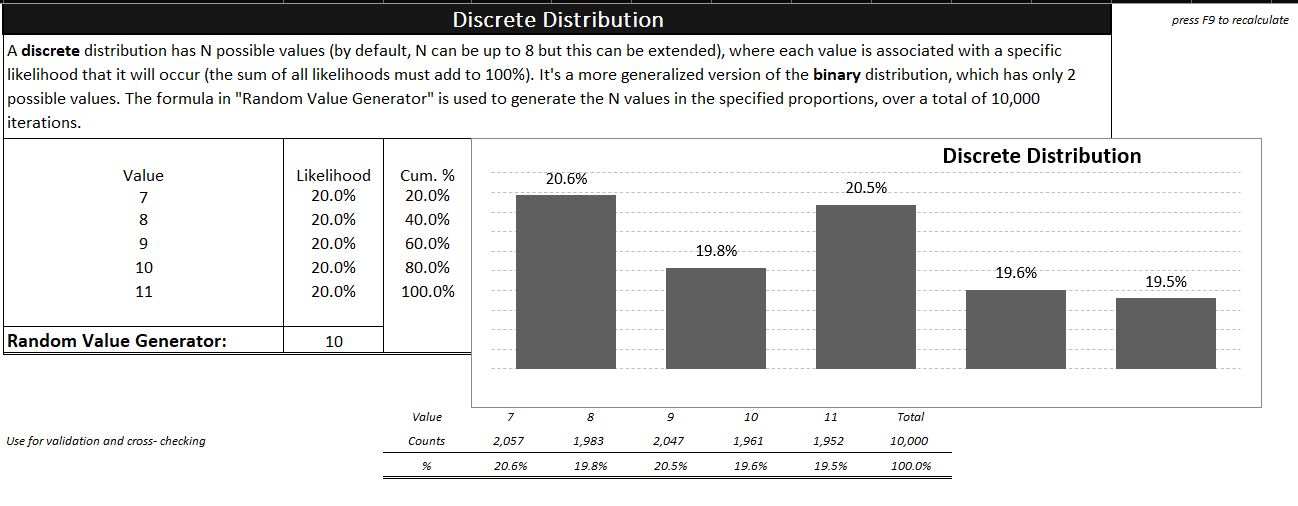
\includegraphics[width=\linewidth]{figures/discrete_threats_percentile.png}}}
  \caption{We ran a\index{Monte Carlo simulation} Monte Carlo simulation of 10,000 iterations with a discrete distribution to spread random instances between confidence intervals taken from the means of seven year samples. We bounded between 0 and 7 possible \gls{threat} (threats, stalking, harrassment, and terrorism) events over a year.\protect\endnote{\index{sample} Sample size was set equivalent to the City of\index{Chattanooga} Chattanooga to determine the per capita rates for each year over data from \index{American Samoa} American Samoa and\index{California} California.  The medians of those rates were used to set 10\% and 90\%\index{confidence interval} confidence intervals with \index{American Samoa} American Samoa and\index{California} California representing low and high \index{cybercrime} cybercrime counts respectively.}
  \protect\endnote{Monte Carlo Modeling Toolkit authored by Derek E. Brink, \gls{cissp}, \url{www.linkedin.com/in/derekbrink}. March 2023.}
  }
  \label{fig:screenshot-montecarlo-\gls{threat}-count-histo}
\end{figure}

\begin{table}[H]
  \centering
  \caption{Monte Carlo Discrete Simulation Values for Threats, Stalking, Harrassment, and Terrorism}
  \label{tab:discrete_threats_montecarlo}
  \begin{center}
  \begin{tabular}{@{}>{\centering\arraybackslash}
  p{0.20\linewidth} >{\centering\arraybackslash}
  p{0.10\linewidth} >{\centering\arraybackslash}
  p{0.10\linewidth} >{\centering\arraybackslash}
  p{0.10\linewidth} >{\centering\arraybackslash}
  p{0.10\linewidth} >{\centering\arraybackslash}
  p{0.10\linewidth}}
    \toprule
Events
&7
&8
&9
&10
&11
\\
    \midrule
Likelihood    
&20.6\%
&19.8\%
&20.5\%
&19.6\%
&19.5\%
\\
    \bottomrule \end{tabular}
    \end{center}
  \raggedright{A\index{Monte Carlo simulation} Monte Carlo simulation was run using a discrete distribution.  We bounded the simulation between 7 and 11 events.  We assigned a 20\% likelihood to each bin.  The resulting distribution showed the effect of randomness on each possible outcome.}
\end{table}

\begin{figure}[H]
  \centering
  \rotatebox{0}{\scalebox{1}{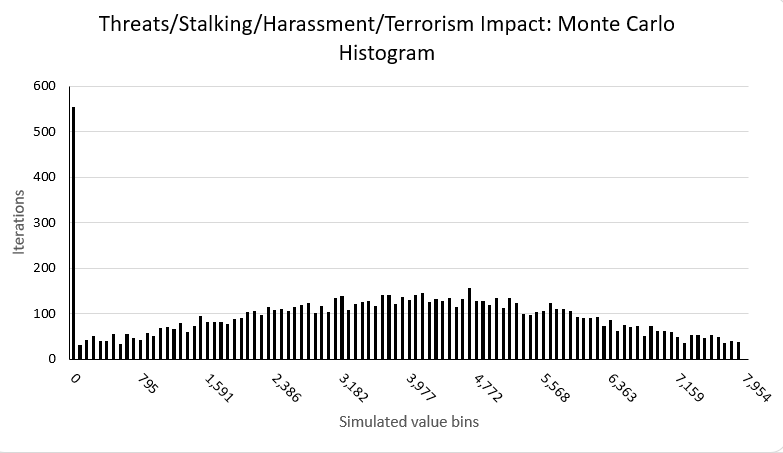
\includegraphics[width=\linewidth]{figures/histogram_threat_impact.png}}}
  \caption{We ran a\index{Monte Carlo simulation} Monte Carlo simulation of 10,000 iterations to spread random instances between confidence intervals taken from means of a seven year sample. We set a lower bound that the event would cost at \$0.  We set an upper bound that the event would cost \$7,954.\protect\endnote{\index{sample} Sample size was set equivalent to the City of\index{Chattanooga} Chattanooga to determine the per capita rates for each year over data from \index{American Samoa} American Samoa and\index{California} California.  The medians of those rates were used to set upper and lower bounds with \index{American Samoa} American Samoa and\index{California} California representing low and high \index{cybercrime} \gls{cybercrime} counts respectively.}
  \protect\endnote{Monte Carlo Modeling Toolkit authored by Derek E. Brink, \gls{cissp}, \url{www.linkedin.com/in/derekbrink}. March 2023.}
  }
  \label{fig:screenshot-montecarlo-threat\index{threat}-impact-histo}
\end{figure}

\begin{figure}[H]
  \centering
  \rotatebox{0}{\scalebox{1}{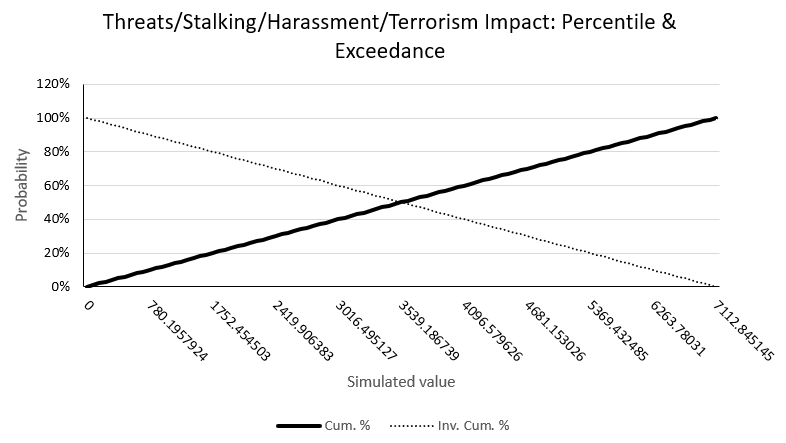
\includegraphics[width=\linewidth]{figures/percent_threats_impact.png}}}
    \[
\mathrm{CI}_{80\%}(\theta) = [\$897,  \$7072]
\]
  
  \caption{A\index{Monte Carlo simulation} Monte Carlo simulation suggests that there is a 90\% probability that\index{threat} threat events will cost \$777.14 or more in a year.  There is a 50\% likelihood that they will cost \$3,544.91 or more in a year.  There is a 10\% chance that they will cost \$6,335.28 or more in a year. \protect\endnote{\index{sample} sample size was set equivalent to the City of\index{Chattanooga} Chattanooga to determine the per capita rates for each year over data from \index{American Samoa} American Samoa and\index{California} California.  The medians of those rates were used to set 10\% and 90\%\index{confidence interval} confidence intervals with \index{American Samoa} American Samoa and\index{California} California representing low and high \index{cybercrime} cybercrime impact values respectively.}
  \protect\endnote{Monte Carlo Modeling Toolkit authored by Derek E. Brink, \gls{cissp}, \url{www.linkedin.com/in/derekbrink}. March 2023.}
  }
  \label{fig:screenshot-montecarlo-\gls{threat}-impact-percent}
\end{figure}
\subsection{Threats to Theft of Data Via Network}
\begin{table}[H]
  \centering
  \caption{Projected In-City Victim Counts, City of\index{Chattanooga} Chattanooga, Theft of Data Via Network}
  \label{tab:chattanoogacrime5}
  \begin{tabular}{@{}
  >{\centering\arraybackslash}p{0.05\linewidth}
  >{\centering\arraybackslash}p{0.25\linewidth}
  >{\centering\arraybackslash}p{0.25\linewidth}
  >{\centering\arraybackslash}p{0.25\linewidth}
  >{\centering\arraybackslash}p{0.05\linewidth} }
    \toprule
  Year&\gls{ipr} and Counterfeit&Identify Theft&\gls{bec}&\\

    \midrule
2016&1&7&4&\endnote{original\protect\url{https://www.ic3.gov/Media/PDF/AnnualReport/2016State/StateReport.aspx\#?s=47} current \protect\url{https://www.ic3.gov/AnnualReport/Reports/2016_IC3Report.pdf}}\\
2017&1&8&4&\endnote{original:\protect\url{https://www.ic3.gov/Media/PDF/AnnualReport/2017State/StateReport.aspx\#?s=47} current: \url{https://www.ic3.gov/AnnualReport/Reports/2017_IC3Report.pdf}}\\
2018&0&10&7&\endnote{original:\protect\url{https://www.ic3.gov/Media/PDF/AnnualReport/2018State/StateReport.aspx\#?s=47} current: \url{https://www.ic3.gov/AnnualReport/Reports/2018_IC3Report.pdf}}\\
2019&1&7&8&\endnote{original:\protect\url{https://www.ic3.gov/Media/PDF/AnnualReport/2019State/StateReport.aspx\#?s=47} current: \url{https://www.ic3.gov/AnnualReport/Reports/2019_IC3Report.pdf}}\\
2020&1&10&6&\endnote{original:\protect\url{https://www.ic3.gov/Media/PDF/AnnualReport/2020State/StateReport.aspx\#?s=47} current: \url{https://www.ic3.gov/AnnualReport/Reports/2020_IC3Report.pdf}}\\
2021&1&13&8&\endnote{original:\protect\url{https://www.ic3.gov/Media/PDF/AnnualReport/2021State/StateReport.aspx\#?s=47} current: \url{https://www.ic3.gov/AnnualReport/Reports/2021_IC3Report.pdf}}\\
2022&0&14&10&\endnote{original:\protect\url{https://www.ic3.gov/Media/PDF/AnnualReport/2022State/StateReport.aspx\#?s=47} current: \url{https://www.ic3.gov/AnnualReport/Reports/2022_IC3Report.pdf}}\\

        \bottomrule \end{tabular}
  \raggedright{Counts deduced from \gls{ic3} Victim Complaints for Tennessee adjusted for a per-capita rate and then multiplied by the city's \index{population} population for that year.}
\end{table}
%%%%%%%%%%%%%%%%%%%%  IPR %%%%%%%%%%%%%%%%%%%%%%%%
%%%%%%%%%%%%%%%%%%%%  INTELLECTUAL PROPERTY RIGHTS (IPR) %%%%%%%%%%%%%%%%%%%%%%%%
\newpage
\subsection{Intellectual Property Rights (\gls{ipr})}\label{sec:ipr}
\subsubsection{Lower Bound Computation}
\[
\begin{bmatrix}
\mathbf{x}_{\text{American Samoa}}^{(\text{count})}\\
\mathbf{x}_{\text{American Samoa}}^{(\text{dollars})}
\end{bmatrix}
=
\begin{bmatrix}
0 & \cdots & 0 & \cdots & 0\\
\$0 & \cdots & \$0 & \cdots & \$0
\end{bmatrix}.
\]
% Columns represent years 2016, \cdots, 2017, \cdots, 2022 for American Samoa IPR/Counterfeit.
% Raw counts: 2016=0, 2017=0, 2022=0.  Raw dollars: 2016=\$0, 2017=\$0, 2022=\$0.
\[
\begin{bmatrix}
\mathbf{x}_{\text{American Samoa}}^{(\text{count scaled to sample population})}\\
\mathbf{x}_{\text{American Samoa}}^{(\text{dollars scaled to sample population})}
\end{bmatrix}
=
\begin{bmatrix}
0 & \cdots & 0 & \cdots & 0\\
\$0 & \cdots & \$0 & \cdots & \$0
\end{bmatrix}.
\]
% Per-capita scaled to Chattanooga population: 2016=0, 2017=0, 2022=0 victims; dollars: all \$0.
\[
\bar{X}_{\text{American Samoa}}^{(m)}
= \frac{1}{N}\sum_{i=1}^{N} X_{\text{American Samoa},i}^{(m)},
\]
\\
\[
\qquad
m \in \{\text{scaled count},\text{scaled dollars}\}
\]
\[
\begin{bmatrix}
\bar{X}_{\text{American Samoa}}^{(\text{scaled count})}\\
\bar{X}_{\text{American Samoa}}^{(\text{scaled dollars})}
\end{bmatrix}
=
\begin{bmatrix}
0.43\\
\$0
\end{bmatrix}.
\]
% Mean of 7-year scaled counts (0,0,0,0,0,3,0) = 3/7 = 0.43.  All dollar values = \$0.
\subsubsection{Upper Bound Computation}
\[
\begin{bmatrix}
\mathbf{x}_{\text{California}}^{(\text{count})}\\
\mathbf{x}_{\text{California}}^{(\text{dollars})}
\end{bmatrix}
=
\begin{bmatrix}
383 & \cdots & 399 & \cdots & 318\\
\$1{,}946{,}413 & \cdots & \$1{,}750{,}437 & \cdots & \$1
\end{bmatrix}.
\]
% Columns represent years 2016, \cdots, 2017, \cdots, 2022 for California IPR/Counterfeit.
% Raw counts: 2016=383, 2017=399, 2022=318.
% Raw state losses: 2016=\$1,946,413; 2017=\$1,750,437; 2022=\$1 (data anomaly in source report).
\[
\begin{bmatrix}
\mathbf{x}_{\text{California}}^{(\text{count scaled to sample population})}\\
\mathbf{x}_{\text{California}}^{(\text{dollars scaled to sample population})}
\end{bmatrix}
=
\begin{bmatrix}
1 & \cdots & 1 & \cdots & 1\\
\$5{,}082 & \cdots & \$4{,}387 & \cdots & \$734
\end{bmatrix}.
\]
% Per-capita scaled to Chattanooga population:
% 2016=1 victim, \$5,082; 2017=1 victim, \$4,387; 2022=1 victim, \$734.
\[
\bar{X}_{\text{California}}^{(m)}
= \frac{1}{N}\sum_{i=1}^{N} X_{\text{California},i}^{(m)},
\]
\\
\[
\qquad
m \in \{\text{scaled count},\text{scaled dollars}\}
\]
\[
\begin{bmatrix}
\bar{X}_{\text{California}}^{(\text{scaled count})}\\
\bar{X}_{\text{California}}^{(\text{scaled dollars})}
\end{bmatrix}
=
\begin{bmatrix}
1.29\\
\$5{,}199
\end{bmatrix}.
\]
% Mean of 7-year scaled counts (1,1,1,1,2,2,1) = 9/7 = 1.29.
% Mean of 7-year scaled losses (\$5082+\$4387+\$4879+\$9228+\$6663+\$5422+\$734)/7 = \$5,199.
\subsubsection{Monte Carlo Simulations for Likelihood and Impact}
\begin{figure}[H]
  \centering
  \rotatebox{0}{\scalebox{1}{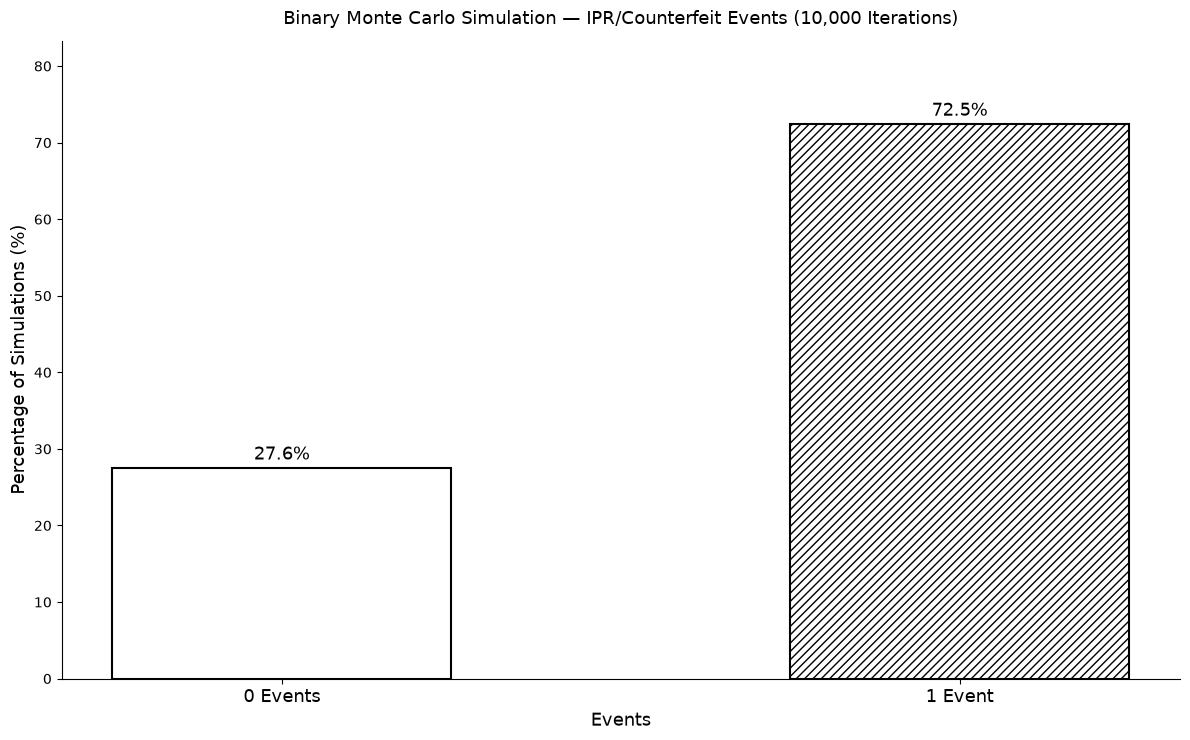
\includegraphics[width=\linewidth]{figures/binary_ipr_count.png}}}
  \caption{We ran a\index{Monte Carlo simulation} Monte Carlo simulation of 10,000 iterations with a \gls{binary} distribution to
  spread random instances between upper and lower bounds taken from the means of seven year samples.
  We bounded between 0 and 1 possible \index{intellectual property rights} intellectual property rights
  (\gls{ipr}) events over a year.\protect\endnote{\index{sample} Sample size was set equivalent to the
  City of\index{Chattanooga} Chattanooga to determine the per capita rates for each year over data
  from \index{American Samoa} American Samoa and\index{California} California.  The means of those
  rates were used to set upper and lower bounds with \index{American Samoa} American Samoa
  and\index{California} California representing low and high \index{cybercrime} \gls{cybercrime} counts
  respectively.}
  \protect\endnote{Monte Carlo Modeling Toolkit authored by Derek E.\ Brink, \gls{cissp},
  \url{www.linkedin.com/in/derekbrink}. March 2023.}
  }
  \label{fig:screenshot-montecarlo-ipr-count-binary}
\end{figure}

When we computed the upper and lower bounds, we recognized that a normal distribution would not fit
well for forecasting likelihood.  We took the mean of the sample from American Samoa for the lower
bound (0.43); we took the mean from the sample from California for the upper bound (1.29); we had a
separation of 0.86 units.  Because the confidence bounds are between 0 and 1, we used a \gls{binary} model.
A \gls{binary} distribution assigns a probability to 0 or 1 events occurring.  We set the probability of
one \gls{ipr}/Counterfeit event at approximately 71.4\%---the midpoint between the lower bound probability
(0.43) and the upper bound probability (capped at 1.0).

\begin{table}[H]
  \centering
  \caption{Monte Carlo \gls{binary} Simulation Values for Intellectual Property Rights (\gls{ipr})}
  \label{tab:binary_ipr_montecarlo}
  \begin{center}
  \begin{tabular}{@{}>{\centering\arraybackslash}
  p{0.30\linewidth} >{\centering\arraybackslash}
  p{0.15\linewidth} >{\centering\arraybackslash}
  p{0.15\linewidth}}
    \toprule
Events  & 0 & 1\\
    \midrule
Likelihood  & 27.6\% & 72.5\%\\
    \bottomrule
  \end{tabular}
  \end{center}
  \raggedright{A\index{Monte Carlo simulation} Monte Carlo simulation was run using a \gls{binary}
  distribution.  We bounded the simulation between 0 and 1 events.  We assigned approximately a
  71.4\% probability to one event occurring.  The resulting distribution showed the effect of
  randomness; the simulation produced 0 events 27.6\% of the time and 1 event 72.5\% of the time.}
\end{table}

\begin{figure}[H]
  \centering
  \rotatebox{0}{\scalebox{1}{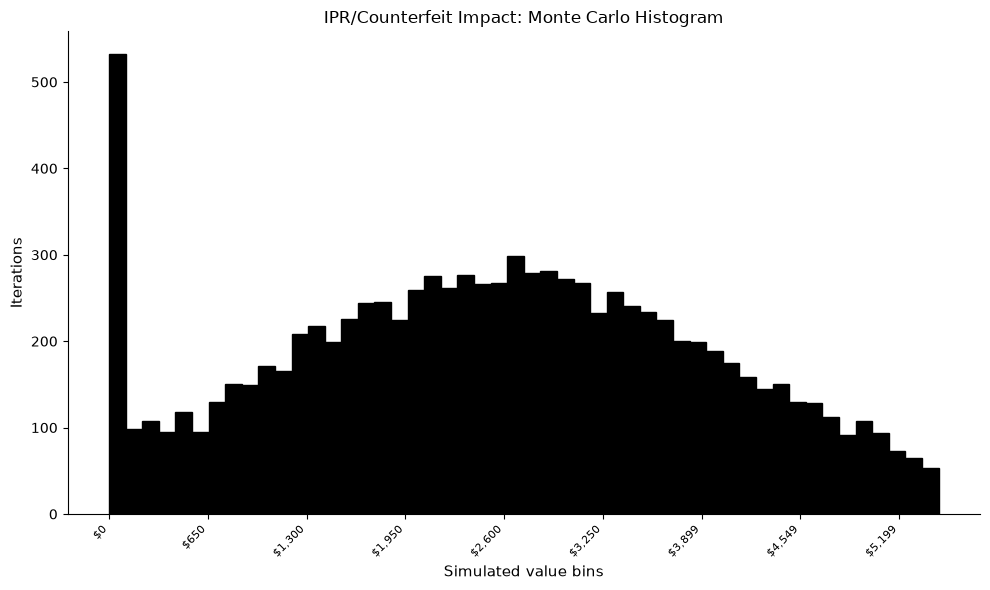
\includegraphics[width=\linewidth]{figures/histogram_ipr_impact_binary.png}}}
  \caption{We ran a\index{Monte Carlo simulation} Monte Carlo simulation of 10,000 iterations with a
  normal distribution to spread random instances between bounds taken from means of seven year
  samples. We set a lower bound that the events would cost at \$0.  We set an upper bound that the
  events would cost \$5{,}199.  \protect\endnote{\index{sample} Sample size was set equivalent to
  the City of\index{Chattanooga} Chattanooga to determine the per capita rates for each year over
  data from \index{American Samoa} American Samoa and\index{California} California.  The means of
  those rates were used to set upper and lower bounds with \index{American Samoa} American Samoa
  and\index{California} California representing low and high \index{cybercrime} \gls{cybercrime} counts
  respectively.}
  \protect\endnote{Monte Carlo Modeling Toolkit authored by Derek E.\ Brink, \gls{cissp},
  \url{www.linkedin.com/in/derekbrink}. March 2023.}
  }
  \label{fig:screenshot-montecarlo-ipr-impact-histo-binary}
\end{figure}

\begin{figure}[H]
  \centering
  \rotatebox{0}{\scalebox{1}{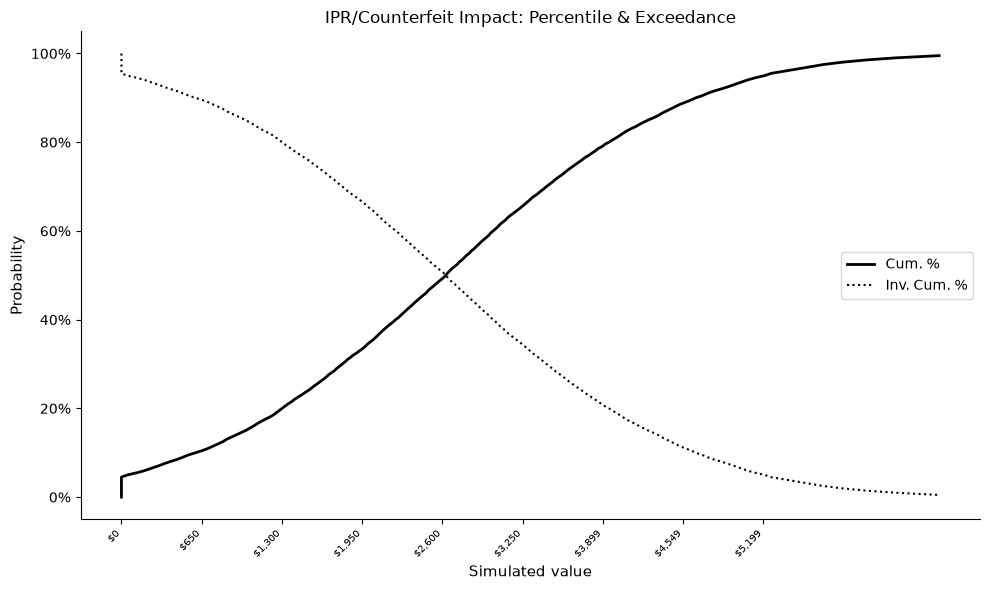
\includegraphics[width=\linewidth]{figures/percent_ipr_impact_binary.png}}}
  \[
\mathrm{CI}_{80\%}(\theta) = [\$602, \$4{,}652]
\]
  \caption{A\index{Monte Carlo simulation} Monte Carlo simulation with a normal distribution
  suggests that there is a 90\% probability that \index{intellectual property rights} intellectual
  property rights events will cost \$602.15 or more in a year.  There is a 50\% likelihood that
  they will cost \$2{,}626.21 or more in a year.  There is a 10\% chance that they will cost
  \$4{,}652.16 or more in a year. \protect\endnote{\index{sample} sample size was set equivalent to
  the City of\index{Chattanooga} Chattanooga to determine the per capita rates for each year over
  data from \index{American Samoa} American Samoa and\index{California} California.  The means of
  those rates were used to set 10\% and 90\%\index{confidence interval} confidence intervals with
  \index{American Samoa} American Samoa and\index{California} California representing low and high
  \index{cybercrime} \gls{cybercrime} impact values respectively.}
  \protect\endnote{Monte Carlo Modeling Toolkit authored by Derek E.\ Brink, \gls{cissp},
  \url{www.linkedin.com/in/derekbrink}. March 2023.}
  }
  \label{fig:screenshot-montecarlo-ipr-impact-percent-binary}
\end{figure}

%%%%%%%%%%%%%%%%%%%%  IDENTITY THEFT %%%%%%%%%%%%%%%%%%%%%%%%
\newpage
\subsection{Identity Theft}\label{sec:identitytheft}
\subsubsection{Lower Bound Computation}
\[
\begin{bmatrix}
\mathbf{x}_{\text{American Samoa}}^{(\text{count})}\\
\mathbf{x}_{\text{American Samoa}}^{(\text{dollars})}
\end{bmatrix}
=
\begin{bmatrix}
0 & \cdots & 0 & \cdots & 2\\
\$0 & \cdots & \$0 & \cdots & \$600
\end{bmatrix}.
\]
% Columns represent years 2016, \cdots, 2017, \cdots, 2022 for American Samoa Identity Theft.
% Raw counts: 2016=0, 2017=0, 2022=2.  Raw dollars: 2016=$0, 2017=$0, 2022=$600.
\[
\begin{bmatrix}
\mathbf{x}_{\text{American Samoa}}^{(\text{count scaled to sample population})}\\
\mathbf{x}_{\text{American Samoa}}^{(\text{dollars scaled to sample population})}
\end{bmatrix}
=
\begin{bmatrix}
0 & \cdots & 0 & \cdots & 8\\
\$0 & \cdots & \$0 & \cdots & \$2{,}100
\end{bmatrix}.
\]
% Per-capita scaled to Chattanooga population: 2016=0, 2017=0, 2022=8 victims; dollars: 2016=$0, 2017=$0, 2022=$2,100.
  \[
\bar{X}_{\text{American Samoa}}^{(m)}
= \frac{1}{N}\sum_{i=1}^{N} X_{\text{American Samoa},i}^{(m)},
\]
\\
\[
\qquad
m \in \{\text{scaled count},\text{scaled dollars}\}
\]
\[
\begin{bmatrix}
\bar{X}_{\text{American Samoa}}^{(\text{scaled count})}\\
\bar{X}_{\text{American Samoa}}^{(\text{scaled dollars})}
\end{bmatrix}
=
\begin{bmatrix}
2\\
\$300
\end{bmatrix}.
\]
\subsubsection{Upper Bound Computation}
\[
\begin{bmatrix}
\mathbf{x}_{\text{California}}^{(\text{count})}\\
\mathbf{x}_{\text{California}}^{(\text{dollars})}
\end{bmatrix}
=
\begin{bmatrix}
2{,}368 & \cdots & 2{,}609 & \cdots & 2{,}854\\
\$17{,}862{,}807 & \cdots & \$10{,}216{,}795 & \cdots & \$27{,}903{,}539
\end{bmatrix}.
\]
% Columns represent years 2016, \cdots, 2017, \cdots, 2022 for California Identity Theft.
\[
\begin{bmatrix}
\mathbf{x}_{\text{California}}^{(\text{count scaled to sample population})}\\
\mathbf{x}_{\text{California}}^{(\text{dollars scaled to sample population})}
\end{bmatrix}
=
\begin{bmatrix}
10 & \cdots & 11 & \cdots & 13\\
\$75{,}434 & \cdots & \$43{,}076 & \cdots & \$127{,}101
\end{bmatrix}.
\]
\[
\bar{X}_{\text{California}}^{(m)}
= \frac{1}{N}\sum_{i=1}^{N} X_{\text{California},i}^{(m)},
\]
\\
\[
\qquad
m \in \{\text{scaled count},\text{scaled dollars}\}
\]
\[
\begin{bmatrix}
\bar{X}_{\text{California}}^{(\text{scaled count})}\\
\bar{X}_{\text{California}}^{(\text{scaled dollars})}
\end{bmatrix}
=
\begin{bmatrix}
12\\
\$118{,}823
\end{bmatrix}.
\]
\subsubsection{Monte Carlo Simulations for Likelihood and Impact}
\begin{figure}[H]
  \centering
  \rotatebox{0}{\scalebox{1}{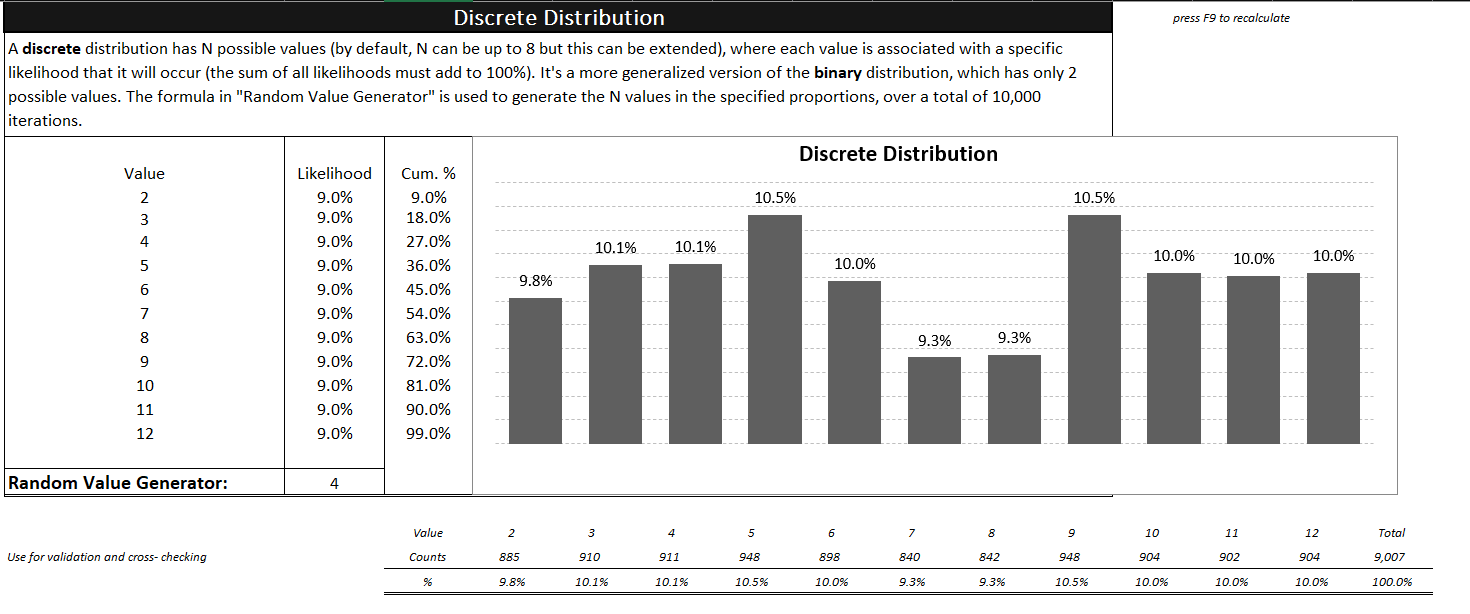
\includegraphics[width=\linewidth]{figures/discrete_idtheft_count.png}}}
  \caption{We ran a\index{Monte Carlo simulation} Monte Carlo simulation of 10,000 iterations with a discrete distribution to spread random instances between confidence intervals taken from the means of seven year samples. We bounded between 2 and 12 possible \index{identity theft}identity theft events over a year.\protect\endnote{\index{sample} Sample size was set equivalent to the City of\index{Chattanooga} Chattanooga to determine the per capita rates for each year over data from \index{American Samoa} American Samoa and\index{California} California.  The means of those rates were used to set 10\% and 90\%\index{confidence interval} confidence intervals with \index{American Samoa} American Samoa and\index{California} California representing low and high \index{cybercrime} cybercrime counts respectively.}
  \protect\endnote{Monte Carlo Modeling Toolkit authored by Derek E. Brink, \gls{cissp}, \url{www.linkedin.com/in/derekbrink}. March 2023.}
  }
  \label{fig:screenshot-montecarlo-idtheft-count-discrete}
\end{figure}
When we computed the upper and lower bounds, we recognized that a normal distribution would not fit well for forecasting likelihood.  We took the mean of the sample from American Samoa for the lower bound (2); we took the mean from the sample from California for the upper bound (12); we had a separation of 10 units.  Therefore, we switched to a discrete model with all 11 options sharing an equal likelihood.
\begin{table}[H]
  \centering
  \caption{Monte Carlo Discrete Simulation Values for Identity Theft}
  \label{tab:discrete_idtheft_montecarlo}
  \begin{center}
  \begin{tabular}{@{}>{\centering\arraybackslash}
  p{0.20\linewidth} >{\centering\arraybackslash}
  p{0.10\linewidth} >{\centering\arraybackslash}
  p{0.10\linewidth} >{\centering\arraybackslash}
  p{0.10\linewidth} >{\centering\arraybackslash}
  p{0.10\linewidth} >{\centering\arraybackslash}
  p{0.10\linewidth} >{\centering\arraybackslash}
  p{0.10\linewidth}}
    \toprule
Events
&2
&3
&4
&5
&6
&7\\
    \midrule
Likelihood    
&8.9\%
&9.5\%
&9.1\%
&8.8\%
&9.4\%
&9.7\%\\
    \bottomrule \end{tabular}
\begin{tabular}{@{}>{\centering\arraybackslash}
  p{0.20\linewidth} >{\centering\arraybackslash}
  p{0.10\linewidth} >{\centering\arraybackslash}
  p{0.10\linewidth} >{\centering\arraybackslash}
  p{0.10\linewidth} >{\centering\arraybackslash}
  p{0.10\linewidth} >{\centering\arraybackslash}
  p{0.10\linewidth}}
    \toprule
Events    
    &8
    &9
    &10
    &11
    &12\\
    \midrule
Likelihood
&9.1\%
&9.4\%
&8.6\%
&8.3\%
&9.2\%\\
    \bottomrule \end{tabular}
    \end{center}
  \raggedright{A\index{Monte Carlo simulation} Monte Carlo simulation was run using a discrete distribution.  We bounded the simulation between 2 and 12 events.  We assigned a $\approx$9.1\% likelihood to each bin.  The resulting distribution showed the effect of randomness on each possible outcome.}
\end{table}

\begin{figure}[H]
  \centering
  \rotatebox{0}{\scalebox{1}{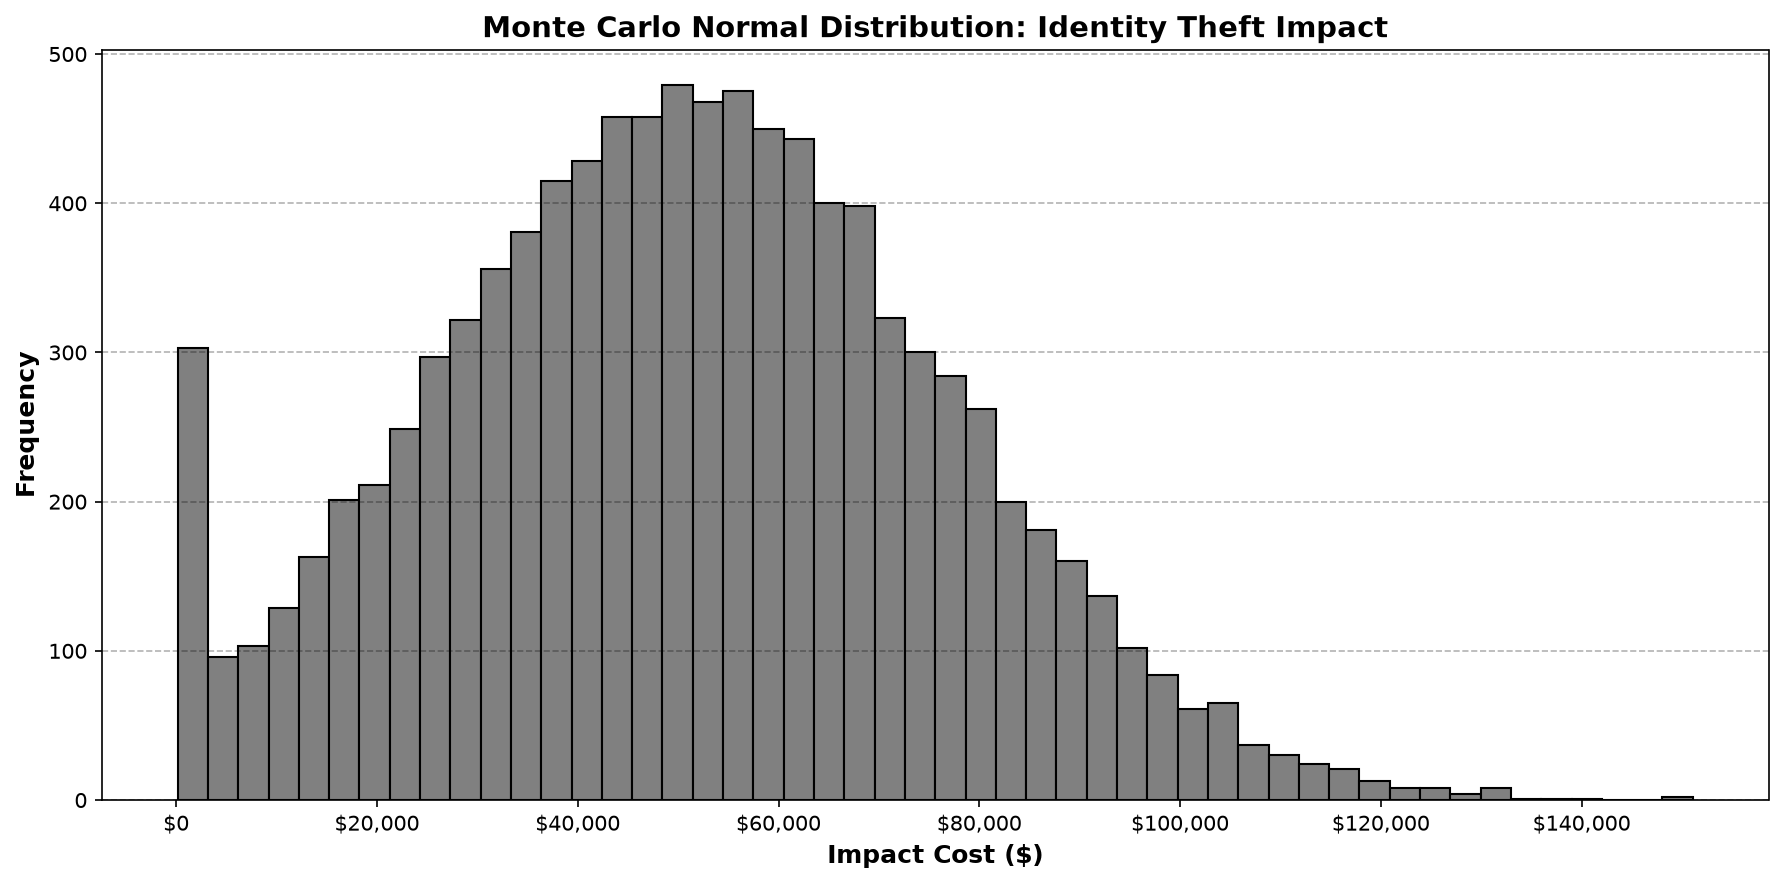
\includegraphics[width=\linewidth]{figures/histogram_idtheft_impact.png}}}
  \caption{We ran a\index{Monte Carlo simulation} Monte Carlo simulation of 10,000 iterations with a normal distribution to spread random instances between bounds taken from means of seven year samples. We set a lower bound that the events would cost at \$0.  We set an upper bound that the events would cost \$118{,}823.  \protect\endnote{\index{sample} Sample size was set equivalent to the City of\index{Chattanooga} Chattanooga to determine the per capita rates for each year over data from \index{American Samoa} American Samoa and\index{California} California.  The means of those rates were used to set upper and lower bounds with \index{American Samoa} American Samoa and\index{California} California representing low and high \index{cybercrime} \gls{cybercrime} impact values respectively.}
  \protect\endnote{Monte Carlo Modeling Toolkit authored by Derek E. Brink, \gls{cissp}, \url{www.linkedin.com/in/derekbrink}. March 2023.}
  }
  \label{fig:screenshot-montecarlo-idtheft-impact-histo}
\end{figure}
\begin{figure}[H]
  \centering
  \rotatebox{0}{\scalebox{1}{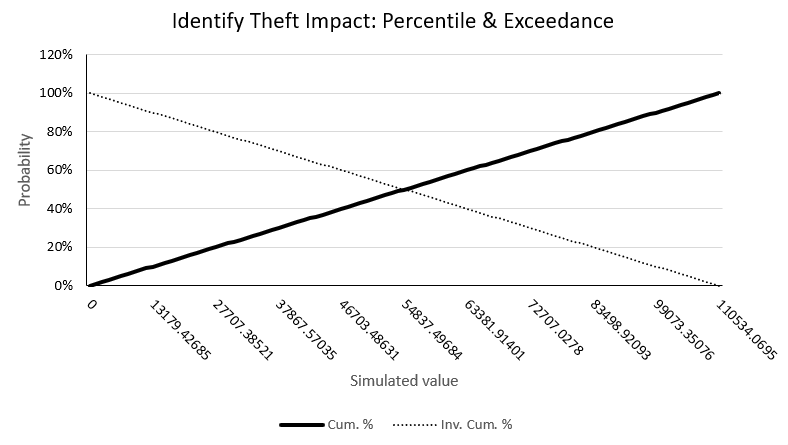
\includegraphics[width=\linewidth]{figures/percent_idtheft_impact.png}}}
  \[
\mathrm{CI}_{80\%}(\theta) = [\$12{,}668, \$98{,}880]
\]
  \caption{A\index{Monte Carlo simulation} Monte Carlo simulation with a normal distribution suggests that there is a 90\% probability that\index{identity theft} identity theft events will cost \$12{,}668 or more in a year.  There is a 50\% likelihood that they will cost \$56{,}158 or more in a year.  There is a 10\% chance that they will cost \$98{,}880 or more in a year. \protect\endnote{\index{sample} sample size was set equivalent to the City of\index{Chattanooga} Chattanooga to determine the per capita rates for each year over data from \index{American Samoa} American Samoa and\index{California} California.  The means of those rates were used to set 10\% and 90\%\index{confidence interval} confidence intervals with \index{American Samoa} American Samoa and\index{California} California representing low and high \index{cybercrime} cybercrime impact values respectively.}
  \protect\endnote{Monte Carlo Modeling Toolkit authored by Derek E. Brink, \gls{cissp}, \url{www.linkedin.com/in/derekbrink}. March 2023.}
  }
  \label{fig:screenshot-montecarlo-idtheft-impact-percent}
\end{figure}
%%%%%%%%%%%%%%%%%%%%  BUSINESS EMAIL COMPROMISE %%%%%%%%%%%%%%%%%%%%
\newpage
\subsection{Business Email Compromise}\label{sec:bec}
\subsubsection{Lower Bound Computation}
\[
\begin{bmatrix}
\mathbf{x}_{\text{American Samoa}}^{(\text{count})}\\
\mathbf{x}_{\text{American Samoa}}^{(\text{dollars})}
\end{bmatrix}
=
\begin{bmatrix}
0 & 0 & \cdots & 2\\
\$0 &\$0 & \cdots &\$960 
\end{bmatrix}.
\]
\[
\begin{bmatrix}
\mathbf{x}_{\text{American Samoa}}^{(\text{count scaled to sample population})}\\
\mathbf{x}_{\text{American Samoa}}^{(\text{dollars scaled to sample population})}
\end{bmatrix}
=
\begin{bmatrix}
0 & 0 & \cdots & 8\\
\$0 & \$0 & \cdots &\$3{,}360
\end{bmatrix}.
\]
  \[
\bar{X}_{\text{American Samoa}}^{(m)}
= \frac{1}{N}\sum_{i=1}^{N} X_{\text{American Samoa},i}^{(m)},
\]
\\
\[
\qquad
m \in \{\text{scaled count},\text{scaled dollars}\}
\]
\[
\begin{bmatrix}
\bar{X}_{\text{American Samoa}}^{(\text{scaled count})}\\
\bar{X}_{\text{American Samoa}}^{(\text{scaled dollars})}
\end{bmatrix}
=
\begin{bmatrix}
4\\
\$13{,}851
\end{bmatrix}.
\]
\subsubsection{Upper Bound Computation}
\[
\begin{bmatrix}
\mathbf{x}_{\text{California}}^{(\text{count})}\\
\mathbf{x}_{\text{California}}^{(\text{dollars})}
\end{bmatrix}
=
\begin{bmatrix}
2{,}155 & 2{,}429 & \cdots & 3{,}269\\
\$69{,}208{,}381 &\$106{,}225{,}791  & \cdots &\$439{,}425{,}357 
\end{bmatrix}.
\]
\[
\begin{bmatrix}
\mathbf{x}_{\text{California}}^{(\text{count scaled to sample population})}\\
\mathbf{x}_{\text{California}}^{(\text{dollars scaled to sample population})}
\end{bmatrix}
=
\begin{bmatrix}
9 & 11 & \cdots & 15\\
\$289{,}037 &\$481{,}055 & \cdots &\$2{,}016{,}329 
\end{bmatrix}.
\]
\[
\bar{X}_{\text{California}}^{(m)}
= \frac{1}{N}\sum_{i=1}^{N} X_{\text{California},i}^{(m)},
\]
\\
\[
\qquad
m \in \{\text{scaled count},\text{scaled dollars}\}
\]
\[
\begin{bmatrix}
\bar{X}_{\text{California}}^{(\text{scaled count})}\\
\bar{X}_{\text{California}}^{(\text{scaled dollars})}
\end{bmatrix}
=
\begin{bmatrix}
13\\
\$784{,}561
\end{bmatrix}.
\]
\subsubsection{Monte Carlo Simulations for Likelihood and Impact}
\begin{figure}[H]
  \centering
  \rotatebox{0}{\scalebox{1}{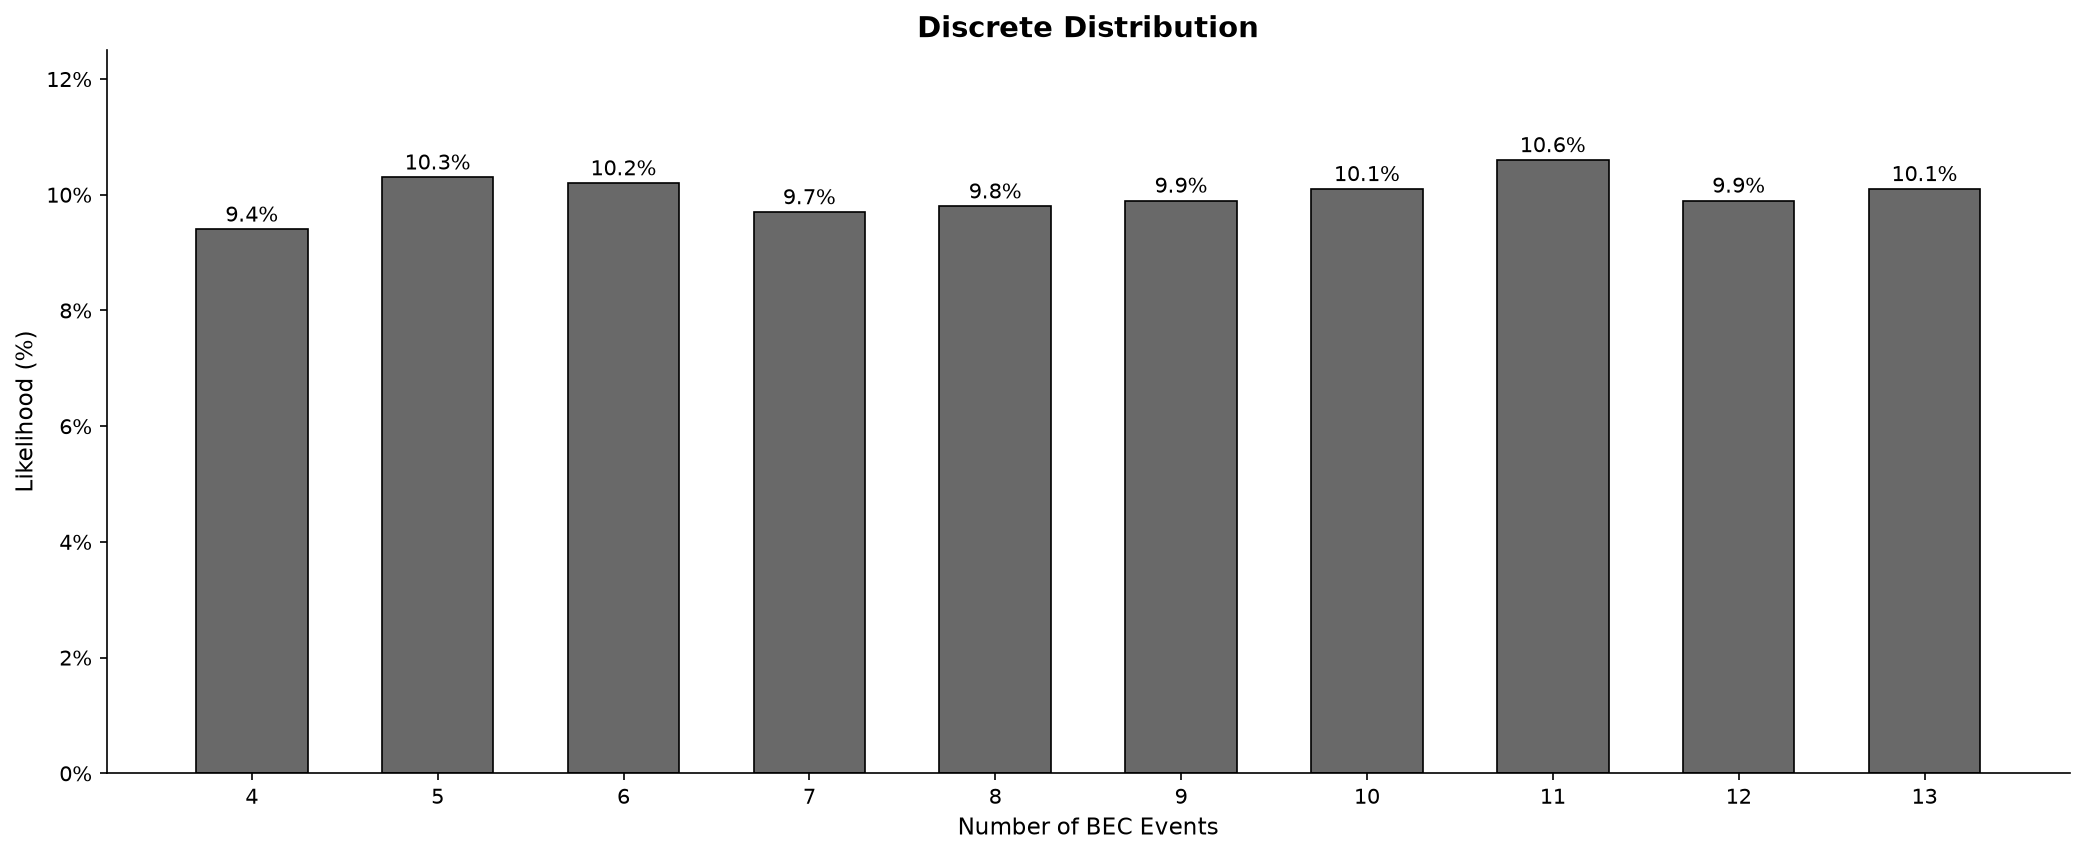
\includegraphics[width=\linewidth]{figures/discrete_bec_count.png}}}
  \caption{We ran a\index{Monte Carlo simulation} Monte Carlo simulation of 10,000 iterations with a discrete distribution to spread random instances between confidence intervals taken from the means of seven year samples. We bounded between 4 and 13 possible \index{business email compromise}business email compromise events over a year.\protect\endnote{\index{sample} Sample size was set equivalent to the City of\index{Chattanooga} Chattanooga to determine the per capita rates for each year over data from \index{American Samoa} American Samoa and\index{California} California.  The means of those rates were used to set lower and upper bounds with \index{American Samoa} American Samoa and\index{California} California representing low and high \index{cybercrime} \gls{cybercrime} counts respectively.}
  \protect\endnote{Monte Carlo Modeling Toolkit authored by Derek E. Brink, \gls{cissp}, \url{www.linkedin.com/in/derekbrink}. March 2023.}
  }
  \label{fig:screenshot-montecarlo-bec-count-discrete}
\end{figure}
When we computed the upper and lower bounds, we recognized that a normal distribution would not fit well for forecasting likelihood.  We took the mean of the sample from American Samoa for the lower bound (4); we took the mean from the sample from California for the upper bound (13); we had a separation of 9 units.  Therefore, we switched to a discrete model with all 10 options sharing an equal likelihood.
\begin{table}[H]
  \centering
  \caption{Monte Carlo Discrete Simulation Values for Business Email Compromise}
  \label{tab:discrete_bec_montecarlo}
  \begin{center}
  \begin{tabular}{@{}>{\centering\arraybackslash}
  p{0.20\linewidth} >{\centering\arraybackslash}
  p{0.10\linewidth} >{\centering\arraybackslash}
  p{0.10\linewidth} >{\centering\arraybackslash}
  p{0.10\linewidth} >{\centering\arraybackslash}
  p{0.10\linewidth} >{\centering\arraybackslash}
  p{0.10\linewidth}}
    \toprule
Events
&4
&5
&6
&7
&8\\
    \midrule
Likelihood    
&9.4\%
&10.3\%
&10.2\%
&9.7\%
&9.8\%\\
    \bottomrule \end{tabular}
\begin{tabular}{@{}>{\centering\arraybackslash}
  p{0.20\linewidth} >{\centering\arraybackslash}
  p{0.10\linewidth} >{\centering\arraybackslash}
  p{0.10\linewidth} >{\centering\arraybackslash}
  p{0.10\linewidth} >{\centering\arraybackslash}
  p{0.10\linewidth} >{\centering\arraybackslash}
  p{0.10\linewidth}}
    \toprule
Events    
    &9
    &10
    &11
    &12
    &13\\
    \midrule
Likelihood
&9.9\%
&10.1\%
&10.6\%
&9.9\%
&10.1\%\\
    \bottomrule \end{tabular}
    \end{center}
  \raggedright{A\index{Monte Carlo simulation} Monte Carlo simulation was run using a discrete distribution.  We bounded the simulation between 4 and 13 events.  We assigned a 10\% likelihood to each bin.  The resulting distribution showed the effect of randomness on each possible outcome.}
\end{table}

\begin{figure}[H]
  \centering
  \rotatebox{0}{\scalebox{1}{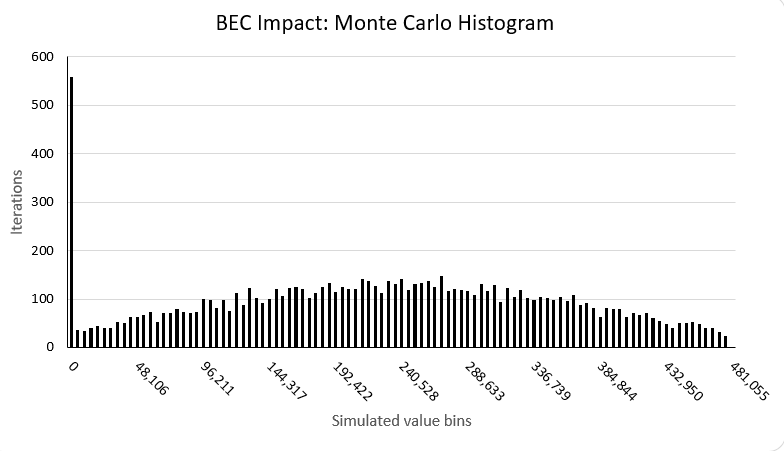
\includegraphics[width=\linewidth]{figures/histogram_bec_impact.png}}}
  \caption{We ran a\index{Monte Carlo simulation} Monte Carlo simulation of 10,000 iterations with a normal distribution to spread random instances between bounds taken from means of seven year samples. We set a lower bound that the events would cost at \$0.  We set an upper bound that the events would cost \$784{,}561.  \protect\endnote{\index{sample} Sample size was set equivalent to the City of\index{Chattanooga} Chattanooga to determine the per capita rates for each year over data from \index{American Samoa} American Samoa and\index{California} California.  The means of those rates were used to set upper and lower bounds with \index{American Samoa} American Samoa and\index{California} California representing low and high \index{cybercrime} \gls{cybercrime} counts respectively.}
  \protect\endnote{Monte Carlo Modeling Toolkit authored by Derek E. Brink, \gls{cissp}, \url{www.linkedin.com/in/derekbrink}. March 2023.}
  }
  \label{fig:screenshot-montecarlo-bec-impact-histo}
\end{figure}
\begin{figure}[H]
  \centering
  \rotatebox{0}{\scalebox{1}{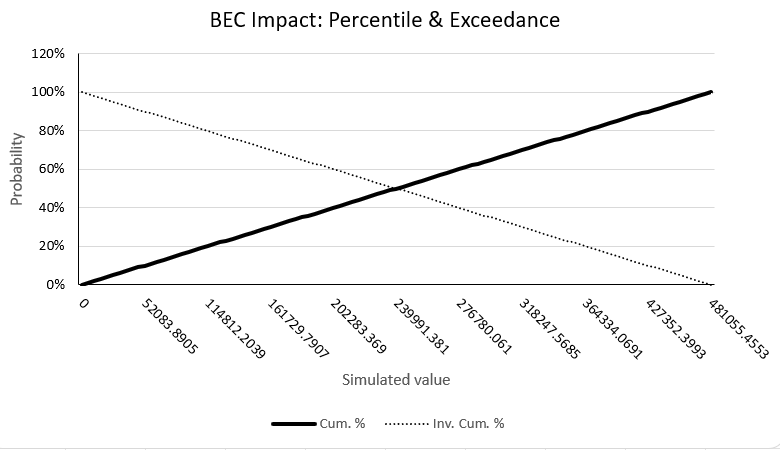
\includegraphics[width=\linewidth]{figures/percent_bec_impact.png}}}
  \[
\mathrm{CI}_{80\%}(\theta) = [\$78{,}456, \$706{,}105]
\]
  \caption{A\index{Monte Carlo simulation} Monte Carlo simulation with a normal distribution suggests that there is a 90\% probability that\index{business email compromise} business email compromise events will cost \$78{,}456 or more in a year.  There is a 50\% likelihood that they will cost \$392{,}281 or more in a year.  There is a 10\% chance that they will cost \$706{,}105 or more in a year. \protect\endnote{\index{sample} sample size was set equivalent to the City of\index{Chattanooga} Chattanooga to determine the per capita rates for each year over data from \index{American Samoa} American Samoa and\index{California} California.  The means of those rates were used to set lower and upper bounds with \index{American Samoa} American Samoa and\index{California} California representing low and high \index{cybercrime} cybercrime impact values respectively.}
  \protect\endnote{Monte Carlo Modeling Toolkit authored by Derek E. Brink, \gls{cissp}, \url{www.linkedin.com/in/derekbrink}. March 2023.}
  }
  \label{fig:screenshot-montecarlo-bec-impact-percent}
\end{figure}
%%%%%%%%%%%%%%%%%%%%% End of graphs %%%%%%%%%%%%%%%%%%%%%%%%%
\section{Analysis}



\section{ANOVA Support Tables}

These supporting tables summarize the adjusted per-capita count and dollar-impact comparisons across the eleven cybercrime\index{cybercrime} categories studied. American Samoa is the lower-bound jurisdiction, Tennessee is the study jurisdiction, and California is the upper-bound jurisdiction.

\subsection{Adjusted Per-Capita Count}

\noindent\textit{Note.} The count comparison tables have been split for readability. Table~\ref{tab:anova-count-means} shows the mean values, while Table~\ref{tab:anova-count-outcomes} shows the hypothesis test outcomes.

\begin{table}[H]
  \centering
  \caption{Adjusted per-capita count: Mean values by category.}
  \label{tab:anova-count-means}
  \small
  \resizebox{0.85\textwidth}{!}{%
  \begin{tabular}{@{}p{0.45\linewidth}rrr@{}}
    \toprule
    Category & AS mean & TN mean & CA mean\\
    \midrule
    Data Breach & 0.43 & 0.43 & 1.00\\
    Personal Data Breach & 5.29 & 14.71 & 25.71\\
    Malware\index{malware} & 0.86 & 0.43 & 0.57\\
    \gls{phishing} & 2.57 & 8.43 & 12.00\\
    Ransomware\index{ransomware} & 0.00 & 0.29 & 1.00\\
    Crimes Against Children & 1.57 & 0.29 & 0.43\\
    Extortion & 4.71 & 14.86 & 22.57\\
    Threats\slash Stalking\slash Harassment\slash Terrorism & 7.29 & 5.00 & 9.17\\
    IPR/Counterfeit & 0.43 & 0.71 & 1.29\\
    Identity Theft & 1.86 & 9.86 & 11.86\\
    BEC & 4.00 & 6.71 & 12.86\\
    \bottomrule
  \end{tabular}%
  }
\end{table}

\begin{table}[H]
  \centering
  \caption{Adjusted per-capita count: Hypothesis test outcomes at $\alpha = 0.05$.}
  \label{tab:anova-count-outcomes}
  \small
  \resizebox{0.85\textwidth}{!}{%
  \begin{tabular}{@{}p{0.45\linewidth}ccc@{}}
    \toprule
    Category & TN > AS & TN < CA & TN between?\\
    \midrule
    Data Breach & No & Yes & No\\
    Personal Data Breach & Yes & Yes & Yes\\
    \gls{malware} & No & Yes & No\\
    Phishing\index{phishing} & Yes & Yes & Yes\\
    Ransomware\index{ransomware} & Yes & Yes & Yes\\
    Crimes Against Children & No & Yes & No\\
    Extortion & Yes & Yes & Yes\\
    Threats\slash Stalking\slash Harassment\slash Terrorism & No & Yes & No\\
    IPR/Counterfeit & Yes & Yes & Yes\\
    Identity Theft & Yes & Yes & Yes\\
    BEC & Yes & Yes & Yes\\
    \bottomrule
  \end{tabular}%
  }
\end{table}

\begin{table}[H]
  \centering
  \caption{One-way ANOVA summary for adjusted per-capita count means.}
  \label{tab:anova-count-summary}
  \begin{tabular}{@{}lr@{}}
    \toprule
    Statistic & Value\\
    \midrule
    Mean(AS) & 2.64\\
    Mean(TN) & 5.61\\
    Mean(CA) & 8.95\\
    Grand mean & 5.73\\
    SSB & 219.50\\
    SSW & 1{,}214.37\\
    F(2,30) & 2.71\\
    p-value & 0.08\\
    \bottomrule
  \end{tabular}
\end{table}

Across the eleven categories, Tennessee exceeded American Samoa in 7 categories, remained below California in 11 categories, and was strictly intermediate in 7 categories. The count ANOVA yielded $F(2,30)=2.71$ with $p=0.08$.

\subsection{Adjusted Per-Capita Dollar Impact}

\noindent\textit{Note.} The dollar-impact comparison tables have been split for readability. Table~\ref{tab:anova-impact-means} shows the mean values, while Table~\ref{tab:anova-impact-outcomes} shows the hypothesis test outcomes.

\begin{table}[H]
  \centering
  \caption{Adjusted per-capita dollar-impact: Mean values by category.}
  \label{tab:anova-impact-means}
  \small
  \resizebox{0.85\textwidth}{!}{%
  \begin{tabular}{@{}p{0.45\linewidth}rrr@{}}
    \toprule
    Category & AS mean & TN mean & CA mean\\
    \midrule
    Data Breach & \$166{,}889.57 & \$7{,}806.88 & \$44{,}615.39\\
    Personal Data Breach & \$270.50 & \$68{,}479.48 & \$212{,}708.42\\
    Malware\index{malware} & \$0.00 & \$84.40 & \$1{,}012.86\\
    Phishing & \$0.00 & \$15{,}994.21 & \$46{,}694.72\\
    Ransomware & \$0.00 & \$655.60 & \$6{,}761.39\\
    Crimes Against Children & \$0.00 & \$7.09 & \$204.40\\
    Extortion & \$300.00 & \$6{,}123.76 & \$43{,}994.25\\
    Threats\slash Stalking\slash Harassment\slash Terrorism & \$0.00 & \$2{,}556.83 & \$7{,}954.95\\
    IPR/Counterfeit & \$0.00 & \$2{,}705.62 & \$5{,}199.29\\
    Identity Theft & \$300.00 & \$35{,}149.68 & \$118{,}823.21\\
    BEC & \$13{,}851.43 & \$492{,}040.82 & \$784{,}560.85\\
    \bottomrule
  \end{tabular}%
  }
\end{table}

\begin{table}[H]
  \centering
  \caption{Adjusted per-capita dollar-impact: Hypothesis test outcomes at $\alpha = 0.05$.}
  \label{tab:anova-impact-outcomes}
  \small
  \resizebox{0.85\textwidth}{!}{%
  \begin{tabular}{@{}p{0.45\linewidth}ccc@{}}
    \toprule
    Category & TN > AS & TN < CA & TN between?\\
    \midrule
    Data Breach & No & Yes & No\\
    Personal Data Breach & Yes & Yes & Yes\\
    Malware\index{malware} & Yes & Yes & Yes\\
    Phishing & Yes & Yes & Yes\\
    \gls{ransomware} & Yes & Yes & Yes\\
    Crimes Against Children & Yes & Yes & Yes\\
    Extortion & Yes & Yes & Yes\\
    Threats\slash Stalking\slash Harassment\slash Terrorism & Yes & Yes & Yes\\
    IPR/Counterfeit & Yes & Yes & Yes\\
    Identity Theft & Yes & Yes & Yes\\
    BEC & Yes & Yes & Yes\\
    \bottomrule
  \end{tabular}%
  }
\end{table}

\begin{table}[H]
  \centering
  \caption{One-way ANOVA summary for adjusted per-capita dollar-impact means.}
  \label{tab:anova-impact-summary}
  \begin{tabular}{@{}lr@{}}
    \toprule
    Statistic & Value\\
    \midrule
    Mean(AS) & \$16{,}510.14\\
    Mean(TN) & \$57{,}418.58\\
    Mean(CA) & \$115{,}684.52\\
    Grand mean & \$63{,}204.41\\
    SSB & 54{,}647{,}924{,}994.67\\
    SSW & 771{,}108{,}736{,}128.26\\
    F(2,30) & 1.06\\
    p-value & 0.36\\
    \bottomrule
  \end{tabular}
\end{table}

Across the eleven categories, Tennessee exceeded American Samoa in 10 categories, remained below California in 11 categories, and was strictly intermediate in 10 categories. The impact ANOVA yielded $F(2,30)=1.06$ with $p=0.36$. Spreadsheet error cells on the impact summary sheets were treated as zero-valued annual observations for averaging.

\noindent\textit{Note.} The American Samoa data-breach impact row contains a non-zero outlier (\$1{,}168{,}227 in 2020) in the workbook, so Tennessee is not intermediate for that impact category.

%----------------------------------------------------------------------------------------
\section{Source data and reshaping}
The source workbook was \texttt{ComputerCrime\_AUG2026\_Impact\_Final\_With\_C5C7\_IFERROR\_CHARTS\_FIXED\_UPDATED.xlsx}. The script extracted the seven annual observations (2016--2022) from the Chattanooga-adjusted summary sheets for American Samoa, Tennessee, and California, then reshaped the eleven \gls{cybercrime} categories into long format.
The long-format \gls{dataset} contains 231 state-year-category rows. 1 workbook error cell was read as missing, so 230 complete observations were used in the mixed-effects model.
The excluded row was State CA, Year 2016, Category Threats\slash Stalking\slash Harassment\slash Terrorism.
\section{Model specification}
The fitted model used State and Category as fixed effects, included their interaction so that within-category contrasts could be estimated directly, and modeled Year as a random intercept:
\[
\mathrm{AdjustedRate}_{ijk} = \beta_0 + \beta_{\mathrm{State}_i} + \beta_{\mathrm{Category}_j} + \beta_{\mathrm{State}\times\mathrm{Category}_{ij}} + b_{\mathrm{Year}_k} + \varepsilon_{ijk}
\]
\section{Type III tests of fixed effects}
\begin{longtable}{lrrrrrr}
\caption{Type III tests of fixed effects from the mixed-effects model.}\label{tab:type3}\\
\toprule
Effect & Sum Sq & Mean Sq & NumDF & DenDF & F value & Pr(>F) \\
\midrule
\endfirsthead
\toprule
Effect & Sum Sq & Mean Sq & NumDF & DenDF & F value & Pr(>F) \\
\midrule
\endhead
State & 1,516.887 & 758.443 & 2 & 191.02 & 32.688 & <0.001 \\
Category & 6,371.227 & 637.123 & 10 & 191.02 & 27.459 & <0.001 \\
State:Category & 2,125.049 & 106.252 & 20 & 191.02 & 4.579 & <0.001 \\
\bottomrule
\end{longtable}
\section{Estimated marginal means}
\begin{longtable}{p{0.25\linewidth}lrrrrr}
\caption{Estimated marginal means by state within category.}\label{tab:emmeans}\\
\toprule
Category & State & emmean & SE & df & lower.CL & upper.CL \\
\midrule
\endfirsthead
\toprule
Category & State & emmean & SE & df & lower.CL & upper.CL \\
\midrule
\endhead
Data Breach & AS & 0.429 & 1.889 & 169.87 & -3.300 & 4.157 \\
Data Breach & TN & 0.429 & 1.889 & 169.87 & -3.300 & 4.157 \\
Data Breach & CA & 1.000 & 1.889 & 169.87 & -2.728 & 4.728 \\
Personal Data Breach & AS & 5.286 & 1.889 & 169.87 & 1.557 & 9.014 \\
Personal Data Breach & TN & 14.714 & 1.889 & 169.87 & 10.986 & 18.443 \\
Personal Data Breach & CA & 25.714 & 1.889 & 169.87 & 21.986 & 29.443 \\
Malware\index{malware} & AS & 0.857 & 1.889 & 169.87 & -2.871 & 4.586 \\
\gls{malware} & TN & 0.429 & 1.889 & 169.87 & -3.300 & 4.157 \\
Malware\index{malware} & CA & 0.571 & 1.889 & 169.87 & -3.157 & 4.300 \\
\gls{phishing} & AS & 2.571 & 1.889 & 169.87 & -1.157 & 6.300 \\
Phishing\index{phishing} & TN & 8.429 & 1.889 & 169.87 & 4.700 & 12.157 \\
Phishing & CA & 12.000 & 1.889 & 169.87 & 8.272 & 15.728 \\
\gls{ransomware} & AS & 0.000 & 1.889 & 169.87 & -3.728 & 3.728 \\
Ransomware & TN & 0.286 & 1.889 & 169.87 & -3.443 & 4.014 \\
Ransomware\index{ransomware} & CA & 1.000 & 1.889 & 169.87 & -2.728 & 4.728 \\
Crimes Against Children & AS & 1.571 & 1.889 & 169.87 & -2.157 & 5.300 \\
Crimes Against Children & TN & 0.286 & 1.889 & 169.87 & -3.443 & 4.014 \\
Crimes Against Children & CA & 0.429 & 1.889 & 169.87 & -3.300 & 4.157 \\
Extortion & AS & 4.714 & 1.889 & 169.87 & 0.986 & 8.443 \\
Extortion & TN & 14.857 & 1.889 & 169.87 & 11.129 & 18.586 \\
Extortion & CA & 22.571 & 1.889 & 169.87 & 18.843 & 26.300 \\
Threats\slash Stalking\slash Harassment\slash Terrorism & AS & 7.286 & 1.889 & 169.87 & 3.557 & 11.014 \\
Threats\slash Stalking\slash Harassment\slash Terrorism & TN & 5.000 & 1.889 & 169.87 & 1.272 & 8.728 \\
Threats\slash Stalking\slash Harassment\slash Terrorism & CA & 9.000 & 2.034 & 177.88 & 4.987 & 13.013 \\
IPR/Counterfeit & AS & 0.429 & 1.889 & 169.87 & -3.300 & 4.157 \\
IPR/Counterfeit & TN & 0.714 & 1.889 & 169.87 & -3.014 & 4.443 \\
IPR/Counterfeit & CA & 1.286 & 1.889 & 169.87 & -2.443 & 5.014 \\
Identity Theft & AS & 1.857 & 1.889 & 169.87 & -1.871 & 5.586 \\
Identity Theft & TN & 9.857 & 1.889 & 169.87 & 6.129 & 13.586 \\
Identity Theft & CA & 11.857 & 1.889 & 169.87 & 8.129 & 15.586 \\
BEC & AS & 4.000 & 1.889 & 169.87 & 0.272 & 7.728 \\
BEC & TN & 6.714 & 1.889 & 169.87 & 2.986 & 10.443 \\
BEC & CA & 12.857 & 1.889 & 169.87 & 9.129 & 16.586 \\
\bottomrule
\end{longtable}
\section{Planned contrasts}
The planned contrasts were Tennessee versus American Samoa and Tennessee versus California within each category, with no multiplicity adjustment because the comparisons were prespecified.

\noindent\textit{Note.} The planned contrasts tables have been split for readability. Table~\ref{tab:contrasts-estimates} shows the point estimates with standard errors and p-values, while Table~\ref{tab:contrasts-intervals} shows the confidence intervals.

\begin{longtable}{p{0.25\linewidth}lrrr}
\caption{Planned contrasts: Point estimates, standard errors, and p-values.}\label{tab:contrasts-estimates}\\
\toprule
Category & contrast & estimate & SE & p.value \\
\midrule
\endfirsthead
\toprule
Category & contrast & estimate & SE & p.value \\
\midrule
\endhead
Data Breach & TN vs AS & -0.000 & 2.575 & 1.000 \\
Data Breach & TN vs CA & -0.571 & 2.575 & 0.825 \\
Personal Data Breach & TN vs AS & 9.429 & 2.575 & <0.001 \\
Personal Data Breach & TN vs CA & -11.000 & 2.575 & <0.001 \\
Malware\index{malware} & TN vs AS & -0.429 & 2.575 & 0.868 \\
Malware & TN vs CA & -0.143 & 2.575 & 0.956 \\
Phishing\index{phishing} & TN vs AS & 5.857 & 2.575 & 0.024 \\
Phishing & TN vs CA & -3.571 & 2.575 & 0.167 \\
Ransomware\index{ransomware} & TN vs AS & 0.286 & 2.575 & 0.912 \\
Ransomware & TN vs CA & -0.714 & 2.575 & 0.782 \\
Crimes Against Children & TN vs AS & -1.286 & 2.575 & 0.618 \\
Crimes Against Children & TN vs CA & -0.143 & 2.575 & 0.956 \\
Extortion & TN vs AS & 10.143 & 2.575 & <0.001 \\
Extortion & TN vs CA & -7.714 & 2.575 & 0.003 \\
Threats\slash Stalking\slash Harassment\slash Terrorism & TN vs AS & -2.286 & 2.575 & 0.376 \\
Threats\slash Stalking\slash Harassment\slash Terrorism & TN vs CA & -4.000 & 2.683 & 0.138 \\
IPR/Counterfeit & TN vs AS & 0.286 & 2.575 & 0.912 \\
IPR/Counterfeit & TN vs CA & -0.571 & 2.575 & 0.825 \\
Identity Theft & TN vs AS & 8.000 & 2.575 & 0.002 \\
Identity Theft & TN vs CA & -2.000 & 2.575 & 0.438 \\
BEC & TN vs AS & 2.714 & 2.575 & 0.293 \\
BEC & TN vs CA & -6.143 & 2.575 & 0.018 \\
\bottomrule
\end{longtable}

\begin{longtable}{p{0.25\linewidth}lrrr}
\caption{Planned contrasts: Degrees of freedom and 95\% confidence intervals.}\label{tab:contrasts-intervals}\\
\toprule
Category & contrast & df & lower.CL & upper.CL \\
\midrule
\endfirsthead
\toprule
Category & contrast & df & lower.CL & upper.CL \\
\midrule
\endhead
Data Breach & TN vs AS & 191.00 & -5.079 & 5.079 \\
Data Breach & TN vs CA & 191.00 & -5.650 & 4.507 \\
Personal Data Breach & TN vs AS & 191.00 & 4.350 & 14.507 \\
Personal Data Breach & TN vs CA & 191.00 & -16.079 & -5.921 \\
\gls{malware} & TN vs AS & 191.00 & -5.507 & 4.650 \\
Malware & TN vs CA & 191.00 & -5.221 & 4.936 \\
\gls{phishing} & TN vs AS & 191.00 & 0.779 & 10.936 \\
\gls{phishing} & TN vs CA & 191.00 & -8.650 & 1.507 \\
\gls{ransomware} & TN vs AS & 191.00 & -4.793 & 5.364 \\
\gls{ransomware} & TN vs CA & 191.00 & -5.793 & 4.364 \\
Crimes Against Children & TN vs AS & 191.00 & -6.364 & 3.793 \\
Crimes Against Children & TN vs CA & 191.00 & -5.221 & 4.936 \\
Extortion & TN vs AS & 191.00 & 5.064 & 15.221 \\
Extortion & TN vs CA & 191.00 & -12.793 & -2.636 \\
Threats\slash Stalking\slash Harassment\slash Terrorism & TN vs AS & 191.00 & -7.364 & 2.793 \\
Threats\slash Stalking\slash Harassment\slash Terrorism & TN vs CA & 191.26 & -9.292 & 1.291 \\
IPR/Counterfeit & TN vs AS & 191.00 & -4.793 & 5.364 \\
IPR/Counterfeit & TN vs CA & 191.00 & -5.650 & 4.507 \\
Identity Theft & TN vs AS & 191.00 & 2.921 & 13.079 \\
Identity Theft & TN vs CA & 191.00 & -7.079 & 3.079 \\
BEC & TN vs AS & 191.00 & -2.364 & 7.793 \\
BEC & TN vs CA & 191.00 & -11.221 & -1.064 \\
\bottomrule
\end{longtable}
\section{Confidence-interval plots}
\begin{figure}[H]
\centering
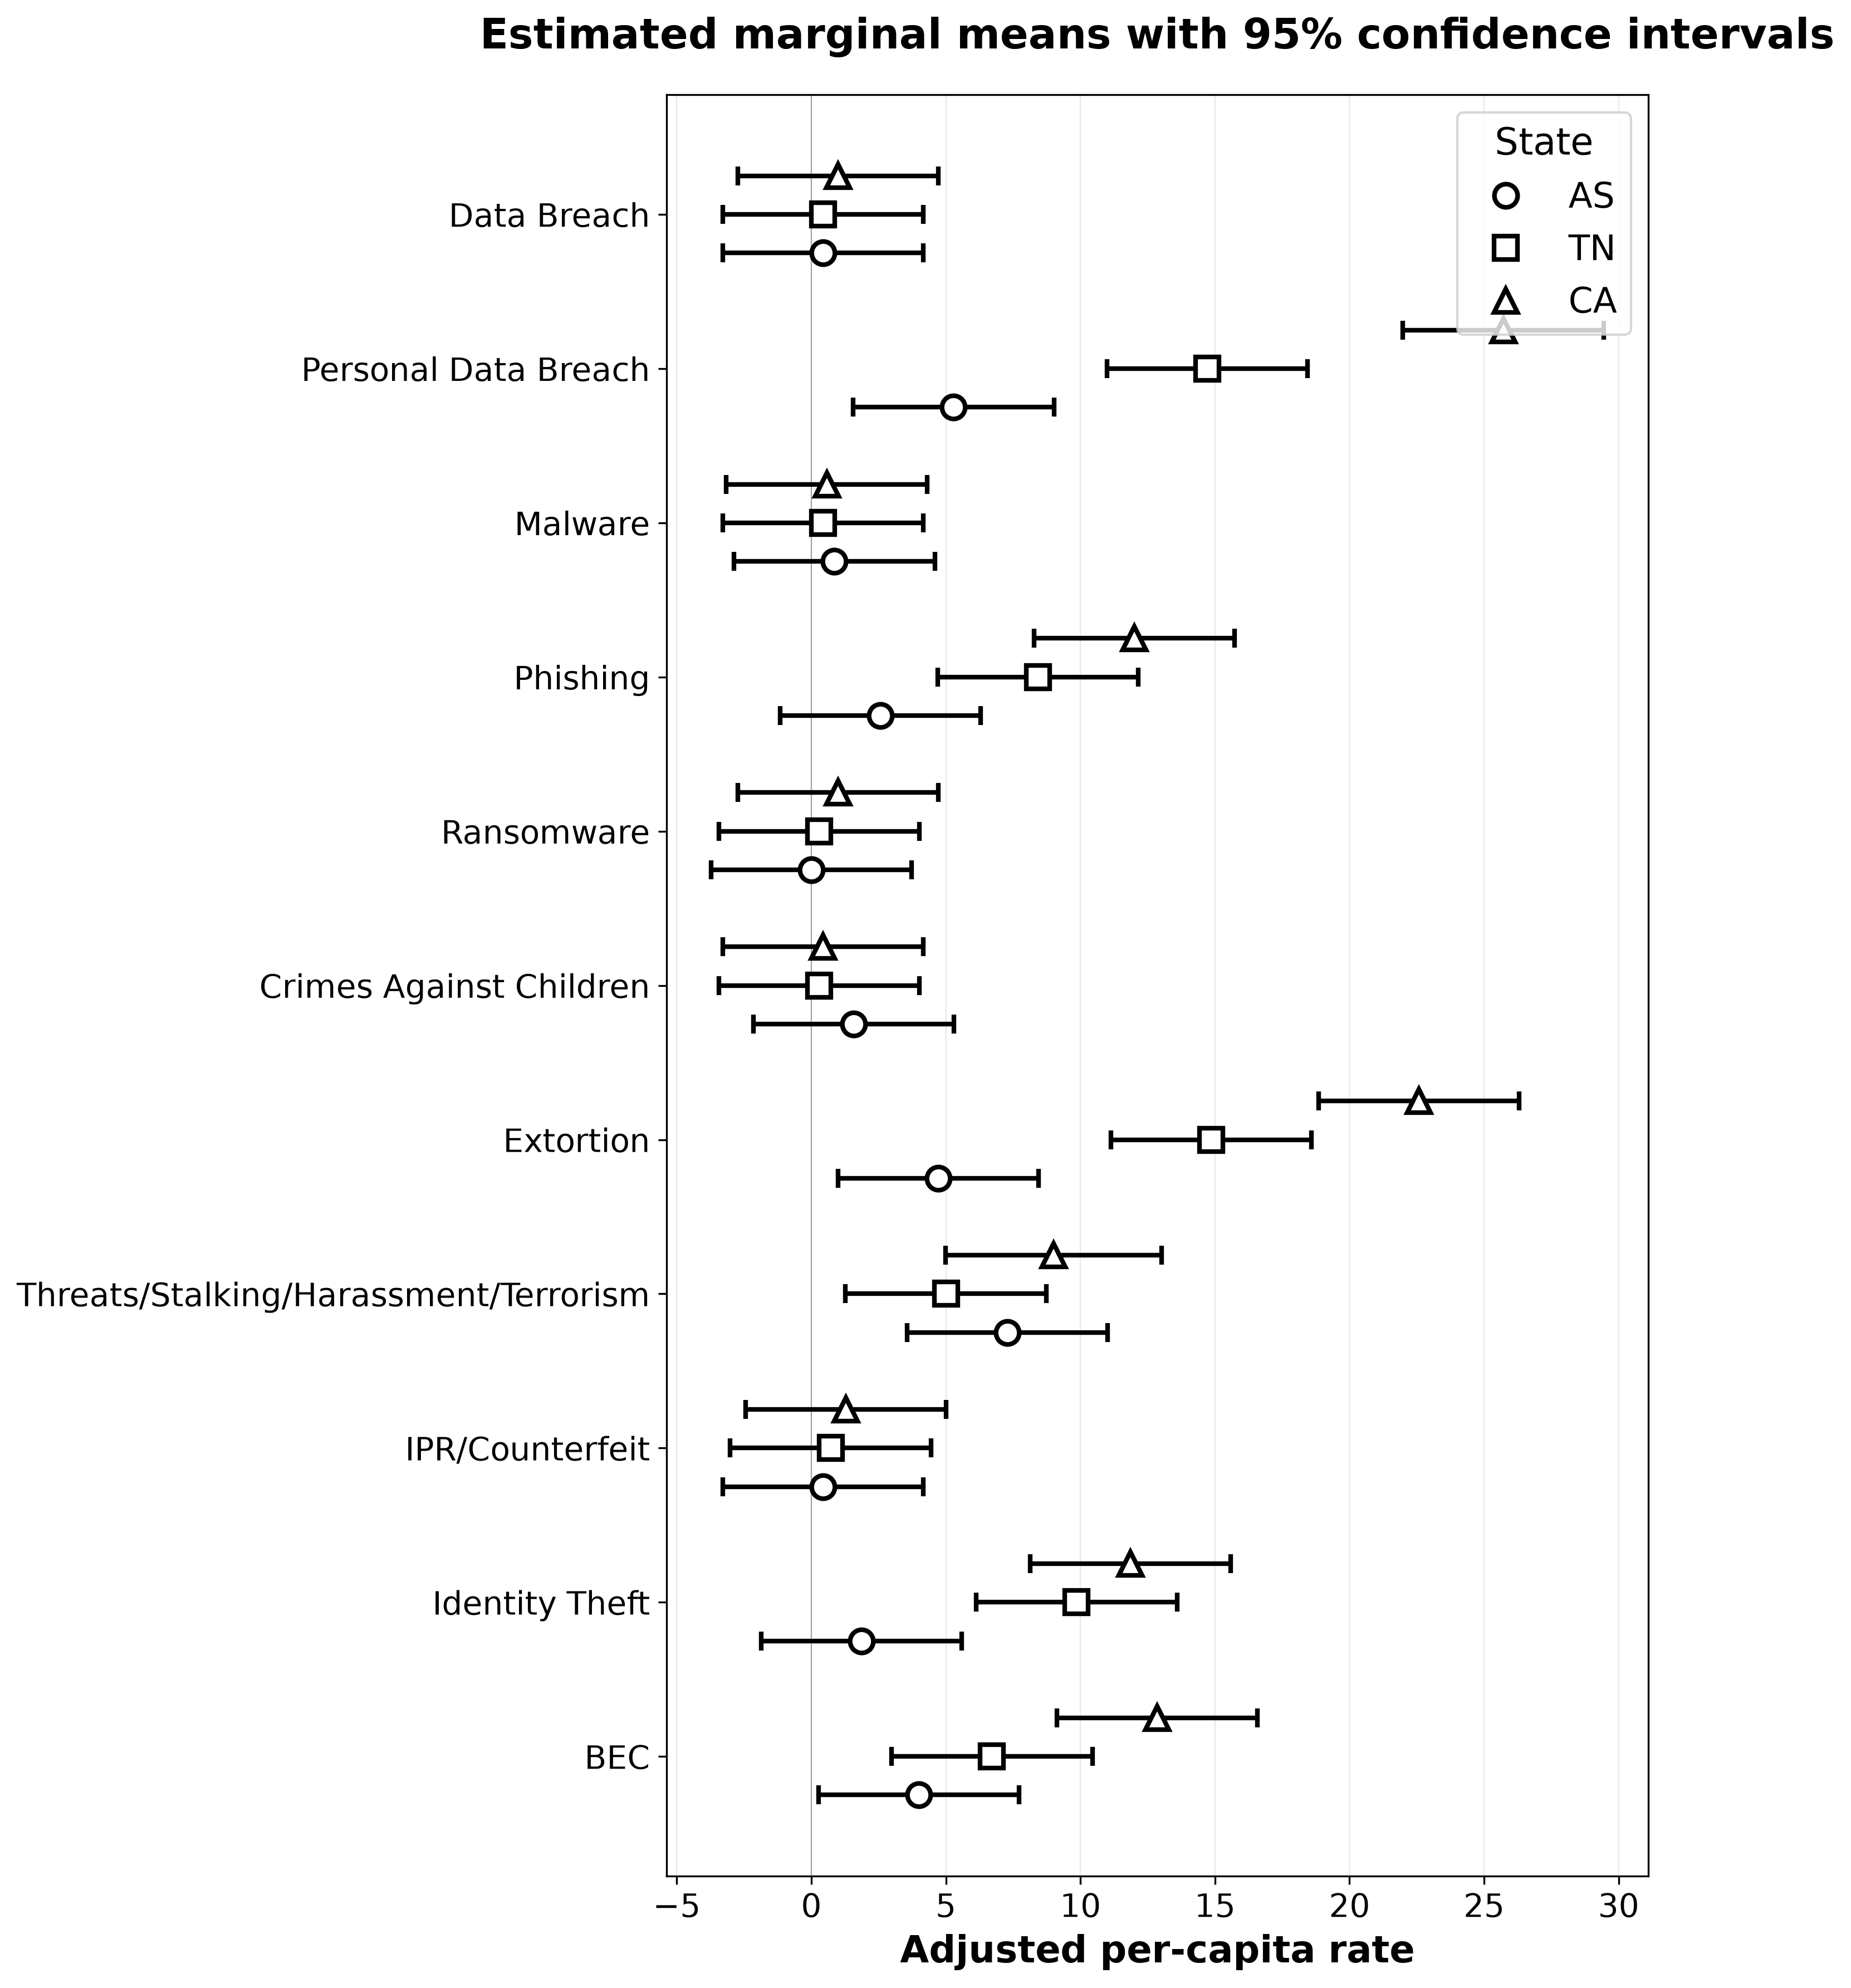
\includegraphics[width=\textwidth]{figures/cybercrime_emmeans_ci.png}
\caption{Estimated marginal means and 95\% confidence intervals.}
\end{figure}
\begin{figure}[H]
\centering
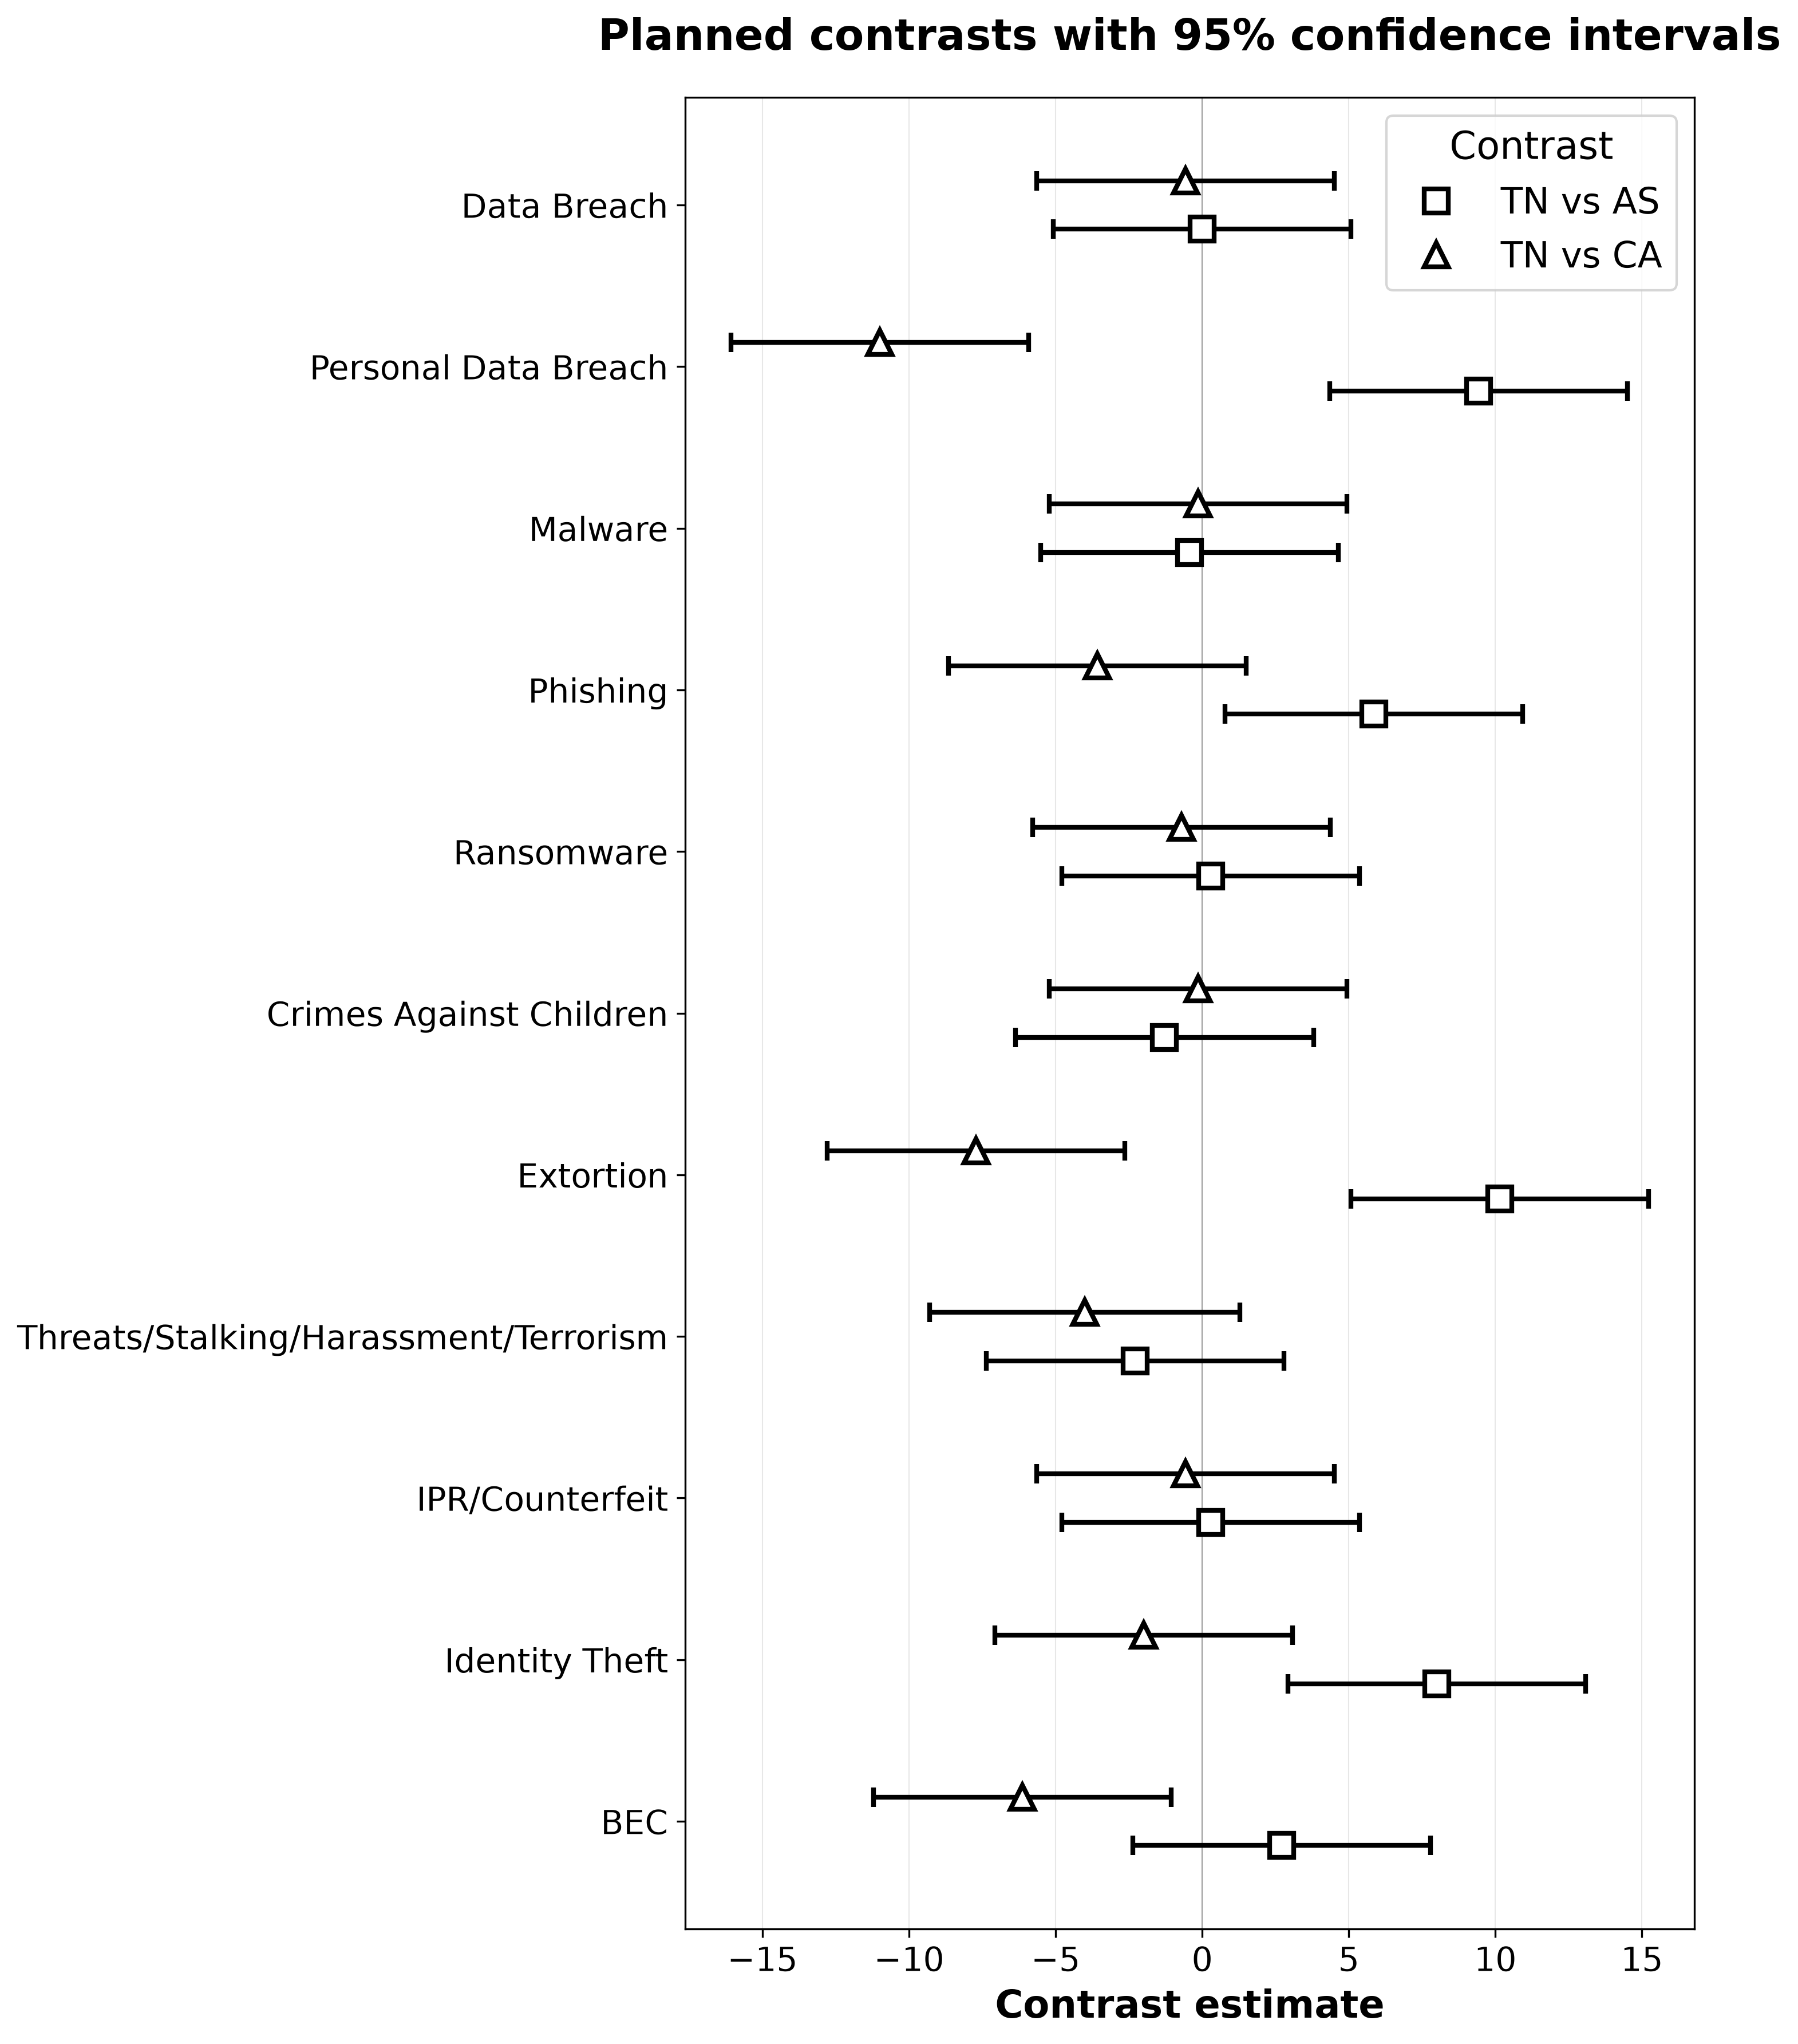
\includegraphics[width=\textwidth]{figures/cybercrime_contrasts_ci.png}
\caption{Planned contrast estimates and 95\% confidence intervals.}
\end{figure}

%----------------------------------------------------------------------------------------


\section{Conditional Framework Findings (AS<TN Screen)}

This section summarizes the conditional workflow:
\begin{enumerate}
  \item Screen categories using adjusted per-capita count means with the condition $AS<TN$.
  \item Keep only categories that pass that count screen.
  \item Re-evaluate count and impact ANOVA using the retained categories.
\end{enumerate}

\subsection{Category-level conditional screen results}

\begin{table}[H]
  \centering
  \caption{Conditional screen on adjusted per-capita count means ($AS<TN$).}
  \label{tab:conditional-screen-count1}
  \small
  \begin{tabular}{@{}p{0.20\linewidth}rrrccc@{}}
    \toprule
    Category & AS mean & TN mean & CA mean\\
    \midrule
    Personal Data Breach & 5.29 & 14.71 & 25.71 \\
    Phishing & 2.57 & 8.43 & 12.00\\
    Ransomware & 0.00 & 0.29 & 1.00 \\
    Extortion & 4.71 & 14.86 & 22.57\\
    IPR/Counterfeit & 0.43 & 0.71 & 1.29 \\
    Identity Theft & 1.86 & 9.86 & 11.86 \\
    BEC & 4.00 & 6.71 & 12.86 \\
    Data Breach & 0.43 & 0.43 & 1.00 \\
    Malware & 0.86 & 0.43 & 0.57 \\
    Crimes Against Children & 1.57 & 0.29 & 0.43 \\
    Threats\slash Stalking\slash Harassment\slash Terrorism & 7.29 & 5.00 & 9.17\\
    \bottomrule
  \end{tabular}
\end{table}

\noindent\textit{Note.} Inclusion in the conditional set is based on $AS<TN$ only. The $TN<CA$ column is shown as a diagnostic and is not used as the inclusion criterion.

\begin{table}[H]
  \centering
  \caption{Conditional screen on adjusted per-capita count means ($AS<TN$).}
  \label{tab:conditional-screen-count2}
  \small
  \begin{tabular}{@{}p{0.20\linewidth}rrrccc@{}}
    \toprule
    Category & $AS<TN$ & $TN<CA$ & Included?\\
    \midrule
    Personal Data Breach & Yes & Yes & Yes\\
    Phishing & Yes & Yes & Yes\\
    Ransomware\index{ransomware} & Yes & Yes & Yes\\
    Extortion & Yes & Yes & Yes\\
    IPR/Counterfeit & Yes & Yes & Yes\\
    Identity Theft & Yes & Yes & Yes\\
    BEC & Yes & Yes & Yes\\
    Data Breach & No & Yes & No\\
    Malware & No & Yes & No\\
    Crimes Against Children & No & Yes & No\\
    Threats\slash Stalking\slash Harassment\slash Terrorism & No & Yes & No\\
    \bottomrule
  \end{tabular}
\end{table}

\noindent\textit{Note.} Inclusion in the conditional set is based on $AS<TN$ only. The $TN<CA$ column is shown as a diagnostic and is not used as the inclusion criterion.
\subsection{Conditional ANOVA summaries}

\begin{table}[H]
  \centering
  \caption{One-way ANOVA summary for adjusted per-capita count means (retained categories only, $n=7$ per state).}
  \label{tab:conditional-count-summary}
  \begin{tabular}{@{}lr@{}}
    \toprule
    Statistic & Value\\
    \midrule
    Mean(AS) & 2.69\\
    Mean(TN) & 7.94\\
    Mean(CA) & 12.47\\
    Grand mean & 7.70\\
    SSB & 335.07\\
    SSW & 770.16\\
    F(2,18) & 3.92\\
    p-value & 0.0387\\
    \bottomrule
  \end{tabular}
\end{table}

\begin{table}[H]
  \centering
  \caption{One-way ANOVA summary for adjusted per-capita dollar-impact means using the same retained count categories ($n=7$ per state).}
  \label{tab:conditional-impact-summary}
  \begin{tabular}{@{}lr@{}}
    \toprule
    Statistic & Value\\
    \midrule
    Mean(AS) & \$2{,}103.13\\
    Mean(TN) & \$88{,}735.60\\
    Mean(CA) & \$174{,}106.02\\
    Grand mean & \$88{,}314.92\\
    SSB & 103{,}549{,}332{,}631.60\\
    SSW & 660{,}271{,}139{,}120.60\\
    F(2,18) & 1.41\\
    p-value & 0.2695\\
    \bottomrule
  \end{tabular}
\end{table}

\subsection{Pass/fail table by p-value threshold}

\begin{table}[H]
  \centering
  \caption{Hypothesis test outcomes at $\alpha=0.05$.}
  \label{tab:conditional-pass-fail1}
  \small
  \begin{tabular}{@{}llp{0.15\linewidth}lp{0.15\linewidth}@{}}
    \toprule
    Analysis & Data scope & p-value\\
    \midrule
    Count ANOVA & Full set (11 categories) & 0.08 \\
    Impact ANOVA & Full set (11 categories) & 0.36 \\
    Count ANOVA & Conditional retained set (7 categories) & 0.0387 \\
    Impact ANOVA & Conditional retained set (same 7 categories) & 0.2695\\
    \bottomrule
  \end{tabular}
\end{table}
\begin{table}[H]
  \centering
  \caption{Hypothesis test outcomes at $\alpha=0.05$.}
  \label{tab:conditional-pass-fail2}
  \small
  \begin{tabular}{@{}lp{0.10\linewidth}cp{0.10\linewidth}cp{0.65\linewidth}@{}}
    \toprule
    Analysis &  Pass/fail & Interpretation\\
    \midrule
    Count ANOVA & Fail & Not strong enough for full-framework inference\\
    Impact ANOVA & Fail & Not strong enough for full-framework inference\\
    Count ANOVA & Pass & Supports conditional count framework in retained categories\\
    Impact ANOVA & Fail & Does not support conditional impact framework\\
    \bottomrule
  \end{tabular}
\end{table}

\noindent\textbf{Conditional conclusion.}
Under the rule ``if a category fails the count screen, exclude it from impact,'' count shows statistical support in the retained subset, but impact still fails to reach significance.

%----------------------------------------------------------------------------------------
\begin{table}[H]
  \centering
  \caption{Summary of Cybercrime Category Analysis References (Part 1 of 2)}
  \label{tab:cybercrime\index{cybercrime}-anova-summary-1}
  \small
  \begin{tabular}{@{}p{0.18\linewidth}p{0.18\linewidth}p{0.18\linewidth}p{0.14\linewidth}p{0.22\linewidth}@{}}
    \toprule
    \textbf{\gls{cybercrime} Category} & \textbf{Object Type} & \textbf{Section Reference} & \textbf{Page Reference} & \textbf{Figure/Table Reference} \\
    \midrule
    Personal Data Breach & Lower Bound Computations & Section~\ref{sec:persdatabreach} & page~\pageref{sec:persdatabreach} & (subsection) \\
    & Upper Bound Computations & Section~\ref{sec:persdatabreach} & page~\pageref{sec:persdatabreach} & (subsection) \\
    & Figure for Monte Carlo simulation & Section~\ref{sec:persdatabreach} & page~\pageref{fig:screenshot-montecarlo-persdatabreach-count-discrete} & Figure~\ref{fig:screenshot-montecarlo-persdatabreach-count-discrete} \\
    & Table of simulation values & Section~\ref{sec:persdatabreach} & page~\pageref{tab:discrete_persdatabreach_montecarlo} & Table~\ref{tab:discrete_persdatabreach_montecarlo} \\
    \midrule
    Phishing\index{phishing} & Lower Bound Computations & Section~\ref{sec:phishing\index{phishing}} & page~\pageref{sec:phishing} & (subsection) \\
    & Upper Bound Computations & Section~\ref{sec:\gls{phishing}} & page~\pageref{sec:phishing} & (subsection) \\
    & Figure for Monte Carlo simulation & Section~\ref{sec:\gls{phishing}} & page~\pageref{fig:screenshot-montecarlo-phishing\index{phishing}-count-discrete} & Figure~\ref{fig:screenshot-montecarlo-phishing-count-discrete} \\
    & Table of simulation values & Section~\ref{sec:phishing} & page~\pageref{tab:discrete_phishing_montecarlo} & Table~\ref{tab:discrete_phishing_montecarlo} \\
    \midrule
    Ransomware\index{ransomware} & Lower Bound Computations & Section~\ref{sec:ransomware} & page~\pageref{sec:\gls{ransomware}} & (subsection) \\
    & Upper Bound Computations & Section~\ref{sec:\gls{ransomware}} & page~\pageref{sec:ransomware} & (subsection) \\
    & Figure for Monte Carlo simulation & Section~\ref{sec:ransomware\index{ransomware}} & page~\pageref{fig:screenshot-montecarlo-ransomware-count-histo} & Figure~\ref{fig:screenshot-montecarlo-ransomware-count-histo} \\
    & Table of simulation values & Section~\ref{sec:\gls{ransomware}} & page~\pageref{sec:ransomware} & (see subsection) \\
    \midrule
    Extortion & Lower Bound Computations & Section~\ref{sec:extortion} & page~\pageref{sec:extortion} & (subsection) \\
    & Upper Bound Computations & Section~\ref{sec:extortion} & page~\pageref{sec:extortion} & (subsection) \\
    & Figure for Monte Carlo simulation & Section~\ref{sec:extortion} & page~\pageref{fig:screenshot-montecarlo-extortion-count-discrete} & Figure~\ref{fig:screenshot-montecarlo-extortion-count-discrete} \\
    & Table of simulation values & Section~\ref{sec:extortion} & page~\pageref{tab:discrete_extortion_montecarlo} & Table~\ref{tab:discrete_extortion_montecarlo} \\
    \bottomrule
  \end{tabular}
\end{table}

\begin{table}[H]
  \centering
  \caption{Summary of Cybercrime Category Analysis References (Part 2 of 2)}
  \label{tab:cybercrime\index{cybercrime}-anova-summary-2}
  \small
  \begin{tabular}{@{}p{0.18\linewidth}p{0.18\linewidth}p{0.18\linewidth}p{0.14\linewidth}p{0.22\linewidth}@{}}
    \toprule
    \textbf{\gls{cybercrime} Category} & \textbf{Object Type} & \textbf{Section Reference} & \textbf{Page Reference} & \textbf{Figure/Table Reference} \\
    \midrule
    IPR/Counterfeit & Lower Bound Computations & Section~\ref{sec:ipr} & page~\pageref{sec:ipr} & (subsection) \\
    & Upper Bound Computations & Section~\ref{sec:ipr} & page~\pageref{sec:ipr} & (subsection) \\
    & Figure for Monte Carlo simulation & Section~\ref{sec:ipr} & page~\pageref{fig:screenshot-montecarlo-ipr-count-binary} & Figure~\ref{fig:screenshot-montecarlo-ipr-count-binary} \\
    & Table of simulation values & Section~\ref{sec:ipr} & page~\pageref{tab:binary_ipr_montecarlo} & Table~\ref{tab:binary_ipr_montecarlo} \\
    \midrule
    Identity Theft & Lower Bound Computations & Section~\ref{sec:identitytheft} & page~\pageref{sec:identitytheft} & (subsection) \\
    & Upper Bound Computations & Section~\ref{sec:identitytheft} & page~\pageref{sec:identitytheft} & (subsection) \\
    & Figure for Monte Carlo simulation & Section~\ref{sec:identitytheft} & page~\pageref{fig:screenshot-montecarlo-idtheft-count-discrete} & Figure~\ref{fig:screenshot-montecarlo-idtheft-count-discrete} \\
    & Table of simulation values & Section~\ref{sec:identitytheft} & page~\pageref{tab:discrete_idtheft_montecarlo} & Table~\ref{tab:discrete_idtheft_montecarlo} \\
    \midrule
    BEC & Lower Bound Computations & Section~\ref{sec:bec} & page~\pageref{sec:bec} & (subsection) \\
    & Upper Bound Computations & Section~\ref{sec:bec} & page~\pageref{sec:bec} & (subsection) \\
    & Figure for Monte Carlo simulation & Section~\ref{sec:bec} & page~\pageref{fig:screenshot-montecarlo-bec-count-discrete} & Figure~\ref{fig:screenshot-montecarlo-bec-count-discrete} \\
    & Table of simulation values & Section~\ref{sec:bec} & page~\pageref{tab:discrete_bec_montecarlo} & Table~\ref{tab:discrete_bec_montecarlo} \\
    \bottomrule
  \end{tabular}
  \raggedright{\small Note: Each cybercrime\index{cybercrime} category includes subsections for Lower Bound Computations and Upper Bound Computations derived from American Samoa (lower) and California (upper) data, scaled to the target population. Monte Carlo simulations were conducted with 10,000 iterations using appropriate distributions (discrete, binary, or normal) based on the data characteristics. The resulting figures and tables provide quantitative assessments of likelihood and impact for each category.}
\end{table}
\section{Results:  Restatement of Graphs}
%%%%%%%%%%%%%%%%%%%% PERSONAL DATA BREACH %%%%%%%%%%%%%%%%%%%%
\newpage
\subsection{Personal Data Breach}\label{sec:persdatabreach}
\subsubsection{Lower Bound Computation}
\[
\begin{bmatrix}
\mathbf{x}_{\text{American Samoa}}^{(\text{count})}\\
\mathbf{x}_{\text{American Samoa}}^{(\text{dollars})}
\end{bmatrix}
=
\begin{bmatrix}
2 & \cdots & 1 & \cdots & 3\\
\$0 & \cdots & \$0 & \cdots & \$11
\end{bmatrix}.
\]
\[
\begin{bmatrix}
\mathbf{x}_{\text{American Samoa}}^{(\text{count scaled to sample population})}\\
\mathbf{x}_{\text{American Samoa}}^{(\text{dollars scaled to sample population})}
\end{bmatrix}
=
\begin{bmatrix}
6 & \cdots & 3 & \cdots & 11.42\\
\$0 & \cdots & \$0 & \cdots & \$0
\end{bmatrix}.
\]
  \[
\bar{X}_{\text{American Samoa}}^{(m)}
= \frac{1}{N}\sum_{i=1}^{N} X_{\text{American Samoa},i}^{(m)},
\]
\\
\[
\qquad
m \in \{\text{scaled count},\text{scaled dollars}\}
\]
\[
\begin{bmatrix}
\bar{X}_{\text{American Samoa}}^{(\text{scaled count})}\\
\bar{X}_{\text{American Samoa}}^{(\text{scaled dollars})}
\end{bmatrix}
=
\begin{bmatrix}
5.35\\
\$270.50
\end{bmatrix}.
\]
\subsubsection{Upper Bound Computation}
\[
\begin{bmatrix}
\mathbf{x}_{\text{California}}^{(\text{count})}\\
\mathbf{x}_{\text{California}}^{(\text{dollars})}
\end{bmatrix}
=
\begin{bmatrix}
4{,}031 & \cdots & 4{,}764 & \cdots & 8{,}196\\
\$8{,}808{,}240 & \cdots & \$9{,}355{,}626 & \cdots & \$153{,}022{,}651
\end{bmatrix}.
\]
\[
\begin{bmatrix}
\mathbf{x}_{\text{California}}^{(\text{count scaled to sample population})}\\
\mathbf{x}_{\text{California}}^{(\text{dollars scaled to sample population})}
\end{bmatrix}
=
\begin{bmatrix}
18 & \cdots & 21 & \cdots & 38.56\\
\$39{,}332.26 & \cdots & \$41{,}240.16 & \cdots & \$709{,}475.44
\end{bmatrix}.
\]
\[
\bar{X}_{\text{California}}^{(m)}
= \frac{1}{N}\sum_{i=1}^{N} X_{\text{California},i}^{(m)},
\]
\\
\[
\qquad
m \in \{\text{scaled count},\text{scaled dollars}\}
\]
\[
\begin{bmatrix}
\bar{X}_{\text{California}}^{(\text{scaled count})}\\
\bar{X}_{\text{California}}^{(\text{scaled dollars})}
\end{bmatrix}
=
\begin{bmatrix}
28.51\\
\$212{,}708.42
\end{bmatrix}.
\]
\subsubsection{Monte Carlo Simulations for Likelihood and Impact}
\begin{figure}[H]
  \centering
  \rotatebox{0}{\scalebox{1}{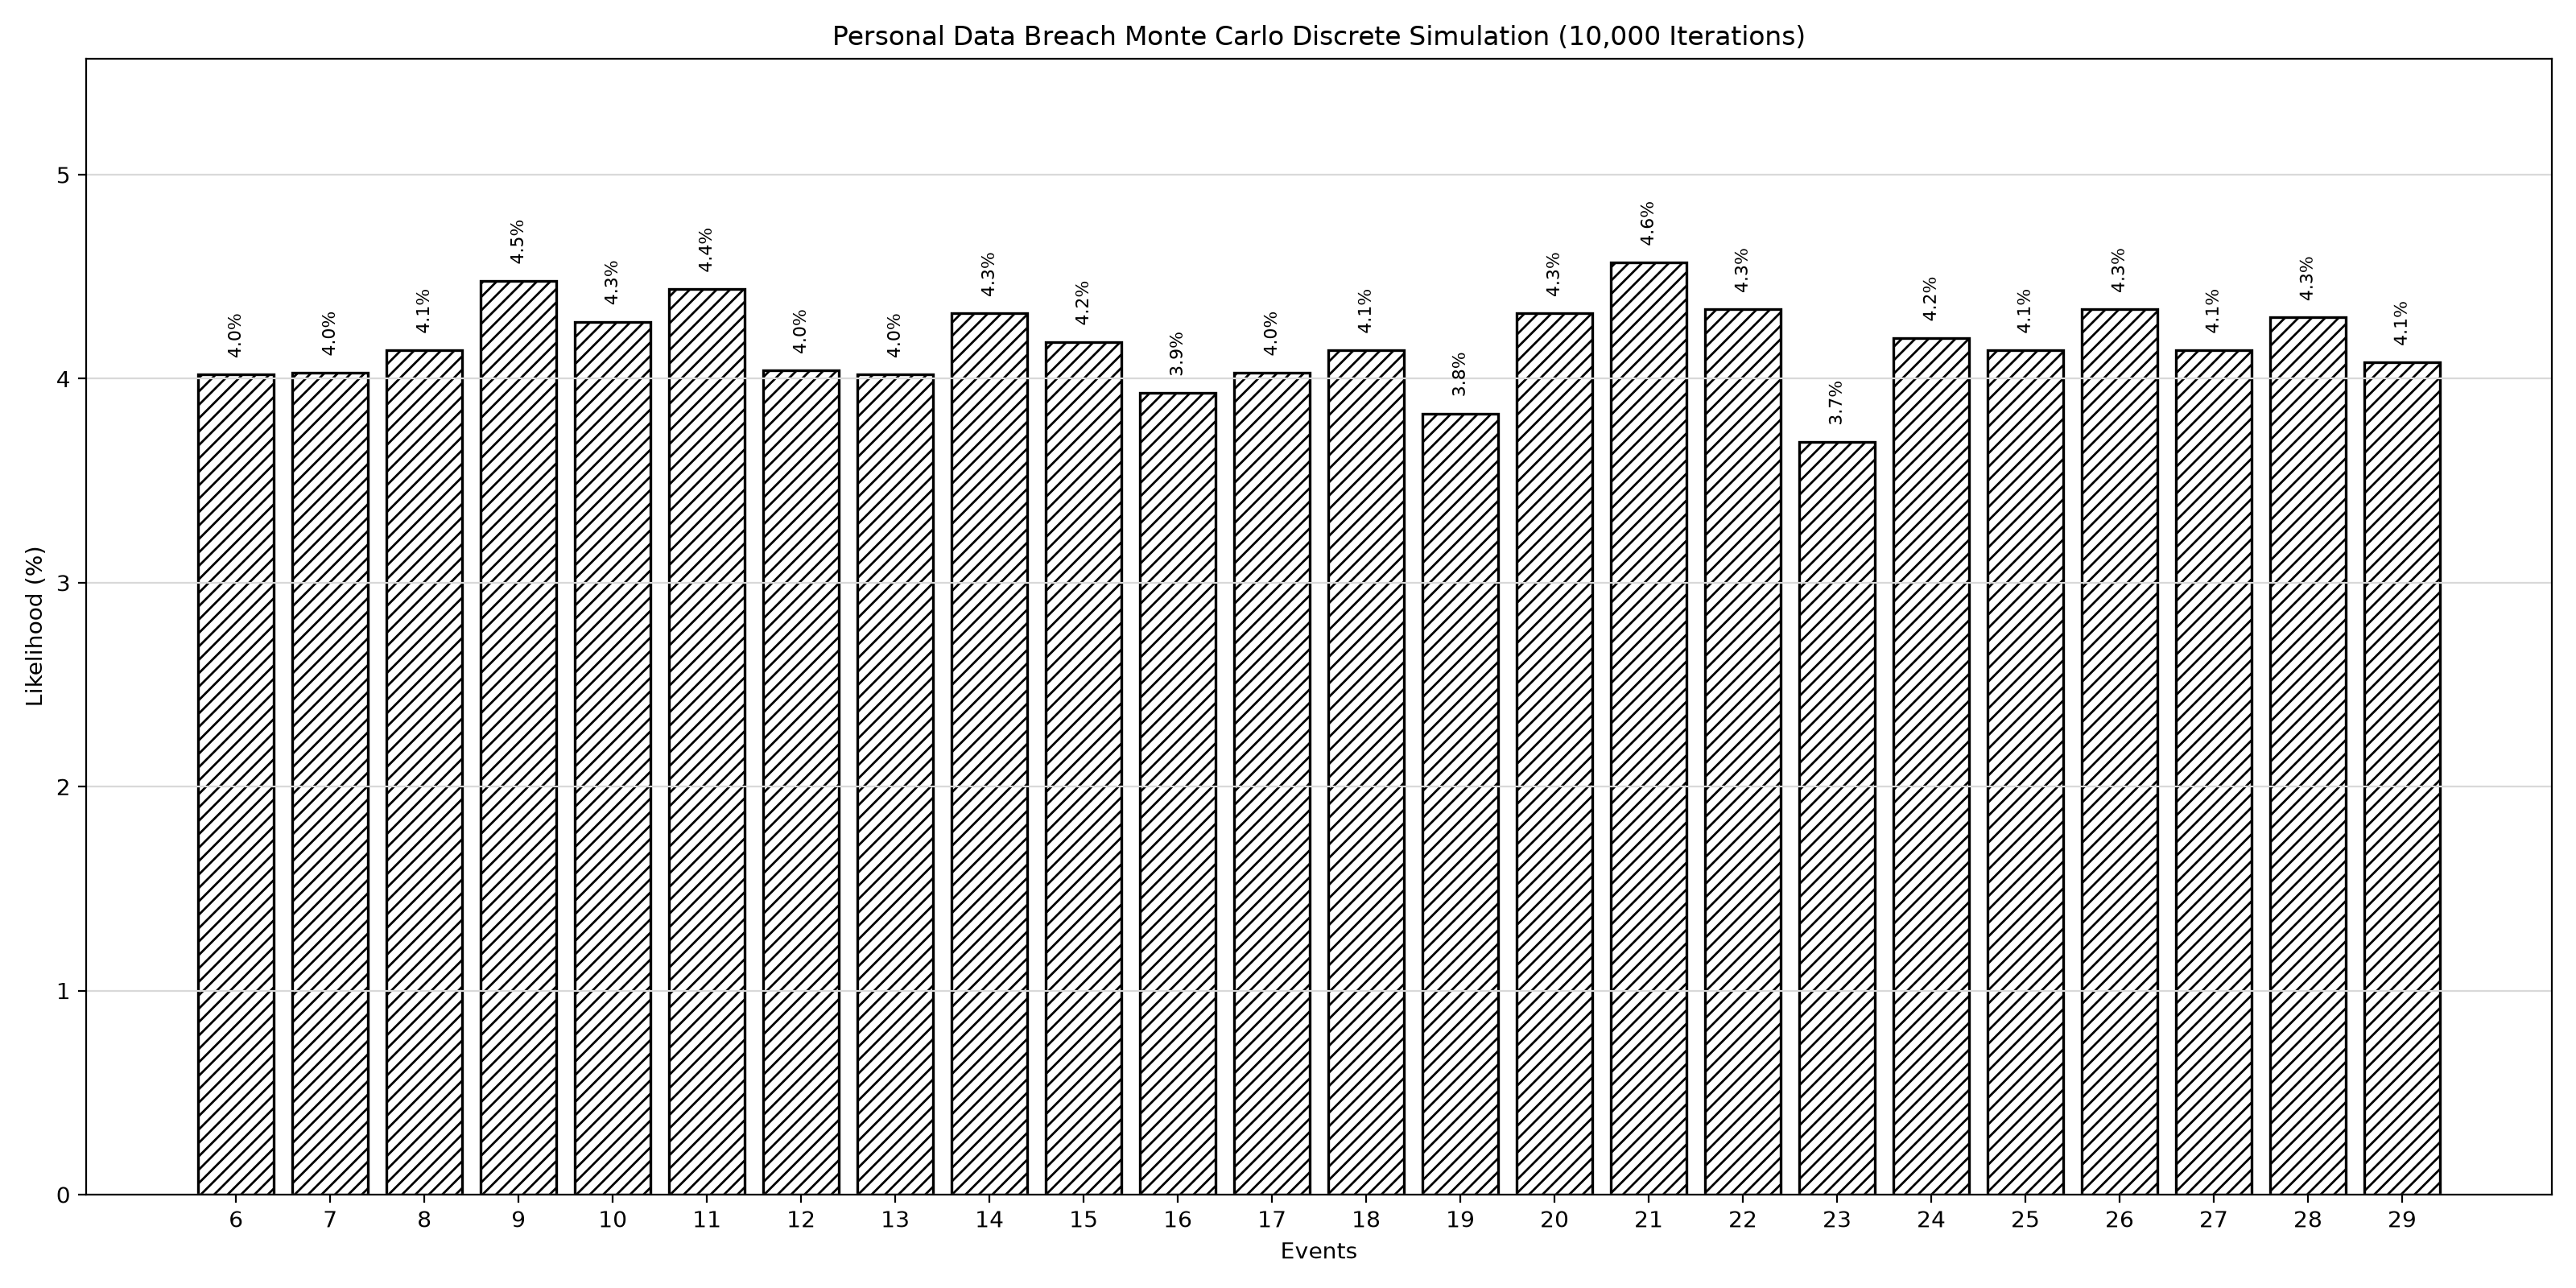
\includegraphics[width=\linewidth]{figures/discrete_persDataBreach_count.png}}}
  \caption{We ran a\index{Monte Carlo simulation} Monte Carlo simulation of 10{,}000 iterations with a discrete distribution to spread random instances between upper and lower bounds taken from the means of seven year samples. We bounded between 6 and 29 possible \index{personal data breach}personal \gls{databreach} events over a year.\protect\endnote{\index{sample} Sample size was set equivalent to the City of\index{Chattanooga} Chattanooga to determine the per capita rates for each year over data from \index{American Samoa} American Samoa and\index{California} California.  The means of those rates were used to set upper and lower bounds with \index{American Samoa} American Samoa and\index{California} California representing low and high \index{cybercrime} \gls{cybercrime} counts respectively.}
  \protect\endnote{Monte Carlo Modeling Toolkit authored by Derek E. Brink, \gls{cissp}, \url{www.linkedin.com/in/derekbrink}. March 2023.}
  }
  \label{fig:screenshot-montecarlo-persdatabreach-count-discrete}
\end{figure}
When we computed the upper and lower bounds, we recognized that a normal distribution would not fit well for forecasting likelihood.  We took the mean of the sample from American Samoa for the lower bound (5.35, rounded to 6); we took the mean from the sample from California for the upper bound (28.51, rounded to 29); we had a separation of 23 units.  Therefore, we switched to a discrete model with all 24 options sharing an equal likelihood.
\begin{table}[H]
  \centering
  \caption{Monte Carlo Discrete Simulation Values for Personal \gls{databreach}}
  \label{tab:discrete_persdatabreach_montecarlo}
  \begin{center}
\begin{tabular}{@{}>{\centering\arraybackslash}p{0.20\linewidth} >{\centering\arraybackslash}p{0.10\linewidth} >{\centering\arraybackslash}p{0.10\linewidth} >{\centering\arraybackslash}p{0.10\linewidth} >{\centering\arraybackslash}p{0.10\linewidth} >{\centering\arraybackslash}p{0.10\linewidth} >{\centering\arraybackslash}p{0.10\linewidth}}
    \toprule
Events
  &6
  &7
  &8
  &9
  &10
  &11\\
    \midrule
Likelihood
  &4.0\%
  &4.0\%
  &4.1\%
  &4.5\%
  &4.3\%
  &4.4\%\\
    \bottomrule \end{tabular}
\begin{tabular}{@{}>{\centering\arraybackslash}p{0.20\linewidth} >{\centering\arraybackslash}p{0.10\linewidth} >{\centering\arraybackslash}p{0.10\linewidth} >{\centering\arraybackslash}p{0.10\linewidth} >{\centering\arraybackslash}p{0.10\linewidth} >{\centering\arraybackslash}p{0.10\linewidth} >{\centering\arraybackslash}p{0.10\linewidth}}
    \toprule
Events
  &12
  &13
  &14
  &15
  &16
  &17\\
    \midrule
Likelihood
  &4.0\%
  &4.0\%
  &4.3\%
  &4.2\%
  &3.9\%
  &4.0\%\\
    \bottomrule \end{tabular}
\begin{tabular}{@{}>{\centering\arraybackslash}p{0.20\linewidth} >{\centering\arraybackslash}p{0.10\linewidth} >{\centering\arraybackslash}p{0.10\linewidth} >{\centering\arraybackslash}p{0.10\linewidth} >{\centering\arraybackslash}p{0.10\linewidth} >{\centering\arraybackslash}p{0.10\linewidth} >{\centering\arraybackslash}p{0.10\linewidth}}
    \toprule
Events
  &18
  &19
  &20
  &21
  &22
  &23\\
    \midrule
Likelihood
  &4.1\%
  &3.8\%
  &4.3\%
  &4.6\%
  &4.3\%
  &3.7\%\\
    \bottomrule \end{tabular}
\begin{tabular}{@{}>{\centering\arraybackslash}p{0.20\linewidth} >{\centering\arraybackslash}p{0.10\linewidth} >{\centering\arraybackslash}p{0.10\linewidth} >{\centering\arraybackslash}p{0.10\linewidth} >{\centering\arraybackslash}p{0.10\linewidth} >{\centering\arraybackslash}p{0.10\linewidth} >{\centering\arraybackslash}p{0.10\linewidth}}
    \toprule
Events
  &24
  &25
  &26
  &27
  &28
  &29\\
    \midrule
Likelihood
  &4.2\%
  &4.1\%
  &4.3\%
  &4.1\%
  &4.3\%
  &4.1\%\\
    \bottomrule \end{tabular}
    \end{center}
  \raggedright{A\index{Monte Carlo simulation} Monte Carlo simulation was run using a discrete distribution.  We bounded the simulation between 6 and 29 events.  We assigned an approximately 4.2\% likelihood to each bin.  A representative 10{,}000-iteration simulation produced the percentages shown above, with no unused event bins.}
\end{table}




%%%%%%%%%%%%%%%%%%%%  \gls{phishing} %%%%%%%%%%%%%%%%%%%%%%%%
\newpage
\subsection{Phishing}\label{sec:phishing}
\subsubsection{Lower Bound Computation}
\[
\begin{bmatrix}
\mathbf{x}_{\text{American Samoa}}^{(\text{count})}\\
\mathbf{x}_{\text{American Samoa}}^{(\text{dollars})}
\end{bmatrix}
=
\begin{bmatrix}
1 & 1 & 0 & 1 & 1 & 1 & 1\\
\$0 &\$0 &\$0 &\$0 &\$0 &\$0 &\$0 
\end{bmatrix}.
\]
\[
\begin{bmatrix}
\mathbf{x}_{\text{American Samoa}}^{(\text{count scaled to sample population})}\\
\mathbf{x}_{\text{American Samoa}}^{(\text{dollars scaled to sample population})}
\end{bmatrix}
=
\begin{bmatrix}
3 & \cdots & 3\\
\$0 & \cdots &\$0
\end{bmatrix}.
\]
  \[
\bar{X}_{\text{American Samoa}}^{(m)}
= \frac{1}{N}\sum_{i=1}^{N} X_{\text{American Samoa},i}^{(m)},
\]
\\
\[
\qquad
m \in \{\text{scaled count},\text{scaled dollars}\}
\]
\[
\begin{bmatrix}
\bar{X}_{\text{American Samoa}}^{(\text{scaled count})}\\
\bar{X}_{\text{American Samoa}}^{(\text{scaled dollars})}
\end{bmatrix}
=
\begin{bmatrix}
3\\
\$0
\end{bmatrix}.
\]
\subsubsection{Upper Bound Computation}
\[
\begin{bmatrix}
\mathbf{x}_{\text{California}}^{(\text{count})}\\
\mathbf{x}_{\text{California}}^{(\text{dollars})}
\end{bmatrix}
=
\begin{bmatrix}
2,059 & 3,302 & \cdots & 2,041\\
\$11,073,447 &\$8,864,419  & \cdots &\$14,628,440 
\end{bmatrix}.
\]
\[
\begin{bmatrix}
\mathbf{x}_{\text{California}}^{(\text{count scaled to sample population})}\\
\mathbf{x}_{\text{California}}^{(\text{dollars scaled to sample population})}
\end{bmatrix}
=
\begin{bmatrix}
9 & 15 & \cdots & 15\\
\$48,402 &\$40,268 & \cdots &\$64,505 
\end{bmatrix}.
\]
\[
\bar{X}_{\text{California}}^{(m)}
= \frac{1}{N}\sum_{i=1}^{N} X_{\text{California},i}^{(m)},
\]
\\
\[
\qquad
m \in \{\text{scaled count},\text{scaled dollars}\}
\]
\[
\begin{bmatrix}
\bar{X}_{\text{California}}^{(\text{scaled count})}\\
\bar{X}_{\text{California}}^{(\text{scaled dollars})}
\end{bmatrix}
=
\begin{bmatrix}
12\\
\$46,695
\end{bmatrix}.
\]
\subsubsection{Monte Carlo Simulations for Likelihood and Impact}
\begin{figure}[H]
  \centering
  \rotatebox{0}{\scalebox{1}{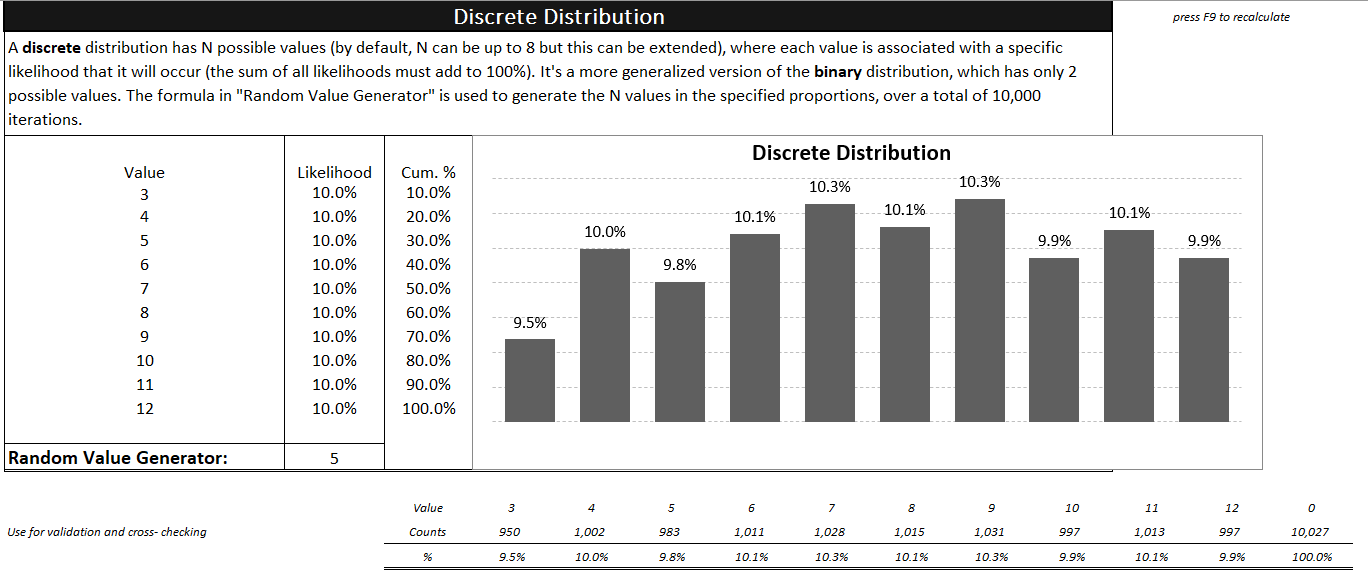
\includegraphics[width=\linewidth]{figures/discrete_phishing_count.png}}}
  \caption{We ran a\index{Monte Carlo simulation} Monte Carlo simulation of 10,000 iterations with a discrete distribution to spread random instances between confidence intervals taken from the means of seven year samples. We bounded between 3 and 12 possible \gls{phishing} events over a year.\protect\endnote{\index{sample} Sample size was set equivalent to the City of\index{Chattanooga} Chattanooga to determine the per capita rates for each year over data from \index{American Samoa} American Samoa and\index{California} California.  The medians of those rates were used to set 10\% and 90\%\index{confidence interval} confidence intervals with \index{American Samoa} American Samoa and\index{California} California representing low and high \index{cybercrime} cybercrime counts respectively.}
  \protect\endnote{Monte Carlo Modeling Toolkit authored by Derek E. Brink, \gls{cissp}, \url{www.linkedin.com/in/derekbrink}. March 2023.}
  }
  \label{fig:screenshot-montecarlo-phishing\index{phishing}-count-discrete}
\end{figure}
When we computed the upper and lower bounds, we recognized that a normal distribution would not fit well for forecasting likelihood.  We took the mean of the sample from American Samoa for the lower bound (3); we took the mean from the sample from California for the upper bound (12); we had a separation of 9 units.  Therefore, we switched to a discrete model with all 10 options sharing an equal likelihood.
\begin{table}[H]
  \centering
  \caption{Monte Carlo Discrete Simulation Values for \gls{phishing}}
  \label{tab:discrete_phishing_montecarlo}
  \begin{center}
  \begin{tabular}{@{}>{\centering\arraybackslash}
  p{0.20\linewidth} >{\centering\arraybackslash}
  p{0.10\linewidth} >{\centering\arraybackslash}
  p{0.10\linewidth} >{\centering\arraybackslash}
  p{0.10\linewidth} >{\centering\arraybackslash}
  p{0.10\linewidth} >{\centering\arraybackslash}
  p{0.10\linewidth}}
    \toprule
Events
&3
&4
&5
&6
&7\\
    \midrule
Likelihood    
&10.4\%
&9.9\%
&9.7\%
&10.0\%
&10.1\%\\
    \bottomrule \end{tabular}
\begin{tabular}{@{}>{\centering\arraybackslash}
  p{0.20\linewidth} >{\centering\arraybackslash}
  p{0.10\linewidth} >{\centering\arraybackslash}
  p{0.10\linewidth} >{\centering\arraybackslash}
  p{0.10\linewidth} >{\centering\arraybackslash}
  p{0.10\linewidth} >{\centering\arraybackslash}
  p{0.10\linewidth}}
    \toprule
Events    
    &8
    &9
    &10
    &11
    &12\\
    \midrule
Likelihood
&10.2\%
&10.1\%
&9.9\%
&9.9\%
&9.9\%\\
    \bottomrule \end{tabular}
    \end{center}
  \raggedright{A\index{Monte Carlo simulation} Monte Carlo simulation was run using a discrete distribution.  We bounded the simulation between 3 and 12 events.  We assigned a 10\% likelihood to each bin.  The resulting distribution showed the effect of randomness on each possible outcome.}
\end{table}

%%%%%%%%%%%%%%%%%%%%  RANSOMWARE %%%%%%%%%%%%%%%%%%%%%%%%
\newpage
\subsection{Ransomware}\label{sec:ransomware}
\subsubsection{Lower Bound Computation}
\[
\begin{bmatrix}
\mathbf{x}_{\text{American Samoa}}^{(\text{count})}\\
\mathbf{x}_{\text{American Samoa}}^{(\text{dollars})}
\end{bmatrix}
=
\begin{bmatrix}
0 & 0 & \cdots & 0\\
\$0 &\$0 & \cdots &\$0 
\end{bmatrix}.
\]
\[
\begin{bmatrix}
\mathbf{x}_{\text{American Samoa}}^{(\text{count scaled to sample population})}\\
\mathbf{x}_{\text{American Samoa}}^{(\text{dollars scaled to sample population})}
\end{bmatrix}
=
\begin{bmatrix}
0 & \cdots & 0\\
\$0 & \cdots &\$0
\end{bmatrix}.
\]
  \[
\bar{X}_{\text{American Samoa}}^{(m)}
= \frac{1}{N}\sum_{i=1}^{N} X_{\text{American Samoa},i}^{(m)},
\]
\\
\[
\qquad
m \in \{\text{scaled count},\text{scaled dollars}\}
\]
\[
\begin{bmatrix}
\bar{X}_{\text{American Samoa}}^{(\text{scaled count})}\\
\bar{X}_{\text{American Samoa}}^{(\text{scaled dollars})}
\end{bmatrix}
=
\begin{bmatrix}
0\\
\$0
\end{bmatrix}.
\]
\subsubsection{Upper Bound Computation}
\[
\begin{bmatrix}
\mathbf{x}_{\text{California}}^{(\text{count})}\\
\mathbf{x}_{\text{California}}^{(\text{dollars})}
\end{bmatrix}
=
\begin{bmatrix}
336 & 222 & \cdots & 296\\
\$260{,}331 &\$600{,}727  & \cdots &\$1{,}945{,}212 
\end{bmatrix}.
\]
\[
\begin{bmatrix}
\mathbf{x}_{\text{California}}^{(\text{count scaled to sample population})}\\
\mathbf{x}_{\text{California}}^{(\text{dollars scaled to sample population})}
\end{bmatrix}
=
\begin{bmatrix}
1 & 1 & \cdots & 1\\
\$775 &\$2{,}706 & \cdots &\$6{,}572 
\end{bmatrix}.
\]
\[
\bar{X}_{\text{California}}^{(m)}
= \frac{1}{N}\sum_{i=1}^{N} X_{\text{California},i}^{(m)},
\]
\\
\[
\qquad
m \in \{\text{scaled count},\text{scaled dollars}\}
\]
\[
\begin{bmatrix}
\bar{X}_{\text{California}}^{(\text{scaled count})}\\
\bar{X}_{\text{California}}^{(\text{scaled dollars})}
\end{bmatrix}
=
\begin{bmatrix}
1.06\\
\$6{,}761
\end{bmatrix}.
\]
\begin{figure}[H]
  \centering
  \rotatebox{0}{\scalebox{1}{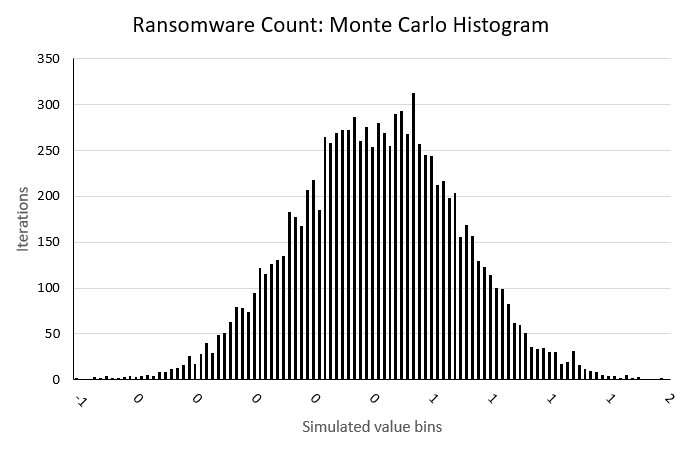
\includegraphics[width=\linewidth]{figures/histogram_ransomware.png}}}
  \caption{We ran a\index{Monte Carlo simulation} Monte Carlo simulation of 10,000 iterations to spread random instances between confidence intervals taken from means of a seven year sample. We bounded between 0 and 1 possible \gls{ransomware} events over a year.\protect\endnote{\index{sample} Sample size was set equivalent to the City of\index{Chattanooga} Chattanooga to determine the per capita rates for each year over data from \index{American Samoa} American Samoa and\index{California} California.  The medians of those rates were used to set upper and lower bounds with \index{American Samoa} American Samoa and\index{California} California representing low and high \index{cybercrime} \gls{cybercrime} counts respectively.}
  \protect\endnote{Monte Carlo Modeling Toolkit authored by Derek E. Brink, \gls{cissp}, \url{www.linkedin.com/in/derekbrink}. March 2023.}
  }
  \label{fig:screenshot-montecarlo-ransomware-count-histo}
\end{figure}

\begin{figure}[H]
  \centering
  \rotatebox{0}{\scalebox{1}{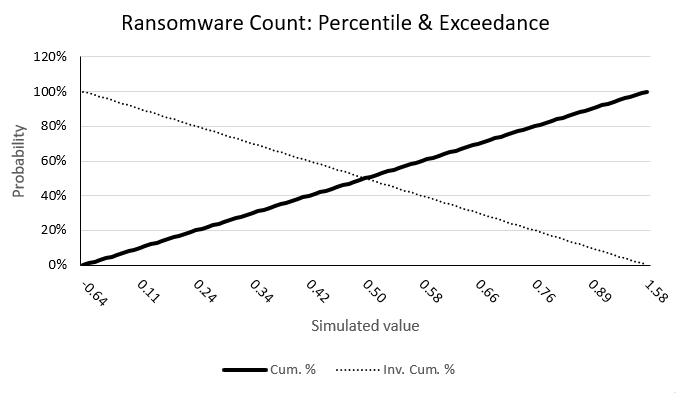
\includegraphics[width=\linewidth]{figures/count_ransomware_percentile.png}}}
  \caption{A\index{Monte Carlo simulation} Monte Carlo simulation suggests that there is a 50\% probability that 0.5 or more\index{ransomware} ransomware events will occur within the \index{sample} sample.  This unusual result is because the confidence bounds are between 0 and 1.  We interpret this as a 50\% probability that one malware event will occur. \protect\endnote{\index{sample} Sample size was set equivalent to the City of\index{Chattanooga} Chattanooga to determine the per capita rates for each year over data from \index{American Samoa} American Samoa and\index{California} California.  The medians of those rates were used to set upper and lower bounds with \index{American Samoa} American Samoa and\index{California} California representing low and high \index{cybercrime} cybercrime counts respectively.}
  \protect\endnote{Monte Carlo Modeling Toolkit authored by Derek E. Brink, \gls{cissp}, \url{www.linkedin.com/in/derekbrink}. March 2023.}
  }
  \label{fig:screenshot-montecarlo-ransomware-count-percent}
\end{figure}

%%%%%%%%%%%%%%%%%%%%  EXTORTION %%%%%%%%%%%%%%%%%%%%%%%%
\newpage
\subsection{Extortion}\label{sec:extortion}
\subsubsection{Lower Bound Computation}
\[
\begin{bmatrix}
\mathbf{x}_{\text{American Samoa}}^{(\text{count})}\\
\mathbf{x}_{\text{American Samoa}}^{(\text{dollars})}
\end{bmatrix}
=
\begin{bmatrix}
2 & 1 & \cdots & 2\\
\$0 & \$0 & \cdots & \$7
\end{bmatrix}.
\]
\[
\begin{bmatrix}
\mathbf{x}_{\text{American Samoa}}^{(\text{count scaled to sample population})}\\
\mathbf{x}_{\text{American Samoa}}^{(\text{dollars scaled to sample population})}
\end{bmatrix}
=
\begin{bmatrix}
6 & \cdots & 7.62\\
\$0 & \cdots & \$300
\end{bmatrix}.
\]
  \[
\bar{X}_{\text{American Samoa}}^{(m)}
= \frac{1}{N}\sum_{i=1}^{N} X_{\text{American Samoa},i}^{(m)},
\]
\\
\[
\qquad
m \in \{\text{scaled count},\text{scaled dollars}\}
\]
\[
\begin{bmatrix}
\bar{X}_{\text{American Samoa}}^{(\text{scaled count})}\\
\bar{X}_{\text{American Samoa}}^{(\text{scaled dollars})}
\end{bmatrix}
=
\begin{bmatrix}
5.60\\
\$300
\end{bmatrix}.
\]
\subsubsection{Upper Bound Computation}
\[
\begin{bmatrix}
\mathbf{x}_{\text{California}}^{(\text{count})}\\
\mathbf{x}_{\text{California}}^{(\text{dollars})}
\end{bmatrix}
=
\begin{bmatrix}
2{,}257 & 2{,}054 & \cdots & 4{,}746\\
\$2{,}413{,}243 & \$1{,}725{,}544 & \cdots & \$22
\end{bmatrix}.
\]
\[
\begin{bmatrix}
\mathbf{x}_{\text{California}}^{(\text{count scaled to sample population})}\\
\mathbf{x}_{\text{California}}^{(\text{dollars scaled to sample population})}
\end{bmatrix}
=
\begin{bmatrix}
10 & 9 & \cdots & 22.33\\
\$10{,}692.26 & \$7{,}560.81 & \cdots & \$2{,}331.31
\end{bmatrix}.
\]
\[
\bar{X}_{\text{California}}^{(m)}
= \frac{1}{N}\sum_{i=1}^{N} X_{\text{California},i}^{(m)},
\]
\\
\[
\qquad
m \in \{\text{scaled count},\text{scaled dollars}\}
\]
\[
\begin{bmatrix}
\bar{X}_{\text{California}}^{(\text{scaled count})}\\
\bar{X}_{\text{California}}^{(\text{scaled dollars})}
\end{bmatrix}
=
\begin{bmatrix}
26.48\\
\$43{,}167.06
\end{bmatrix}.
\]
\subsubsection{Monte Carlo Simulations for Likelihood and Impact}
\begin{figure}[H]
  \centering
  \rotatebox{0}{\scalebox{1}{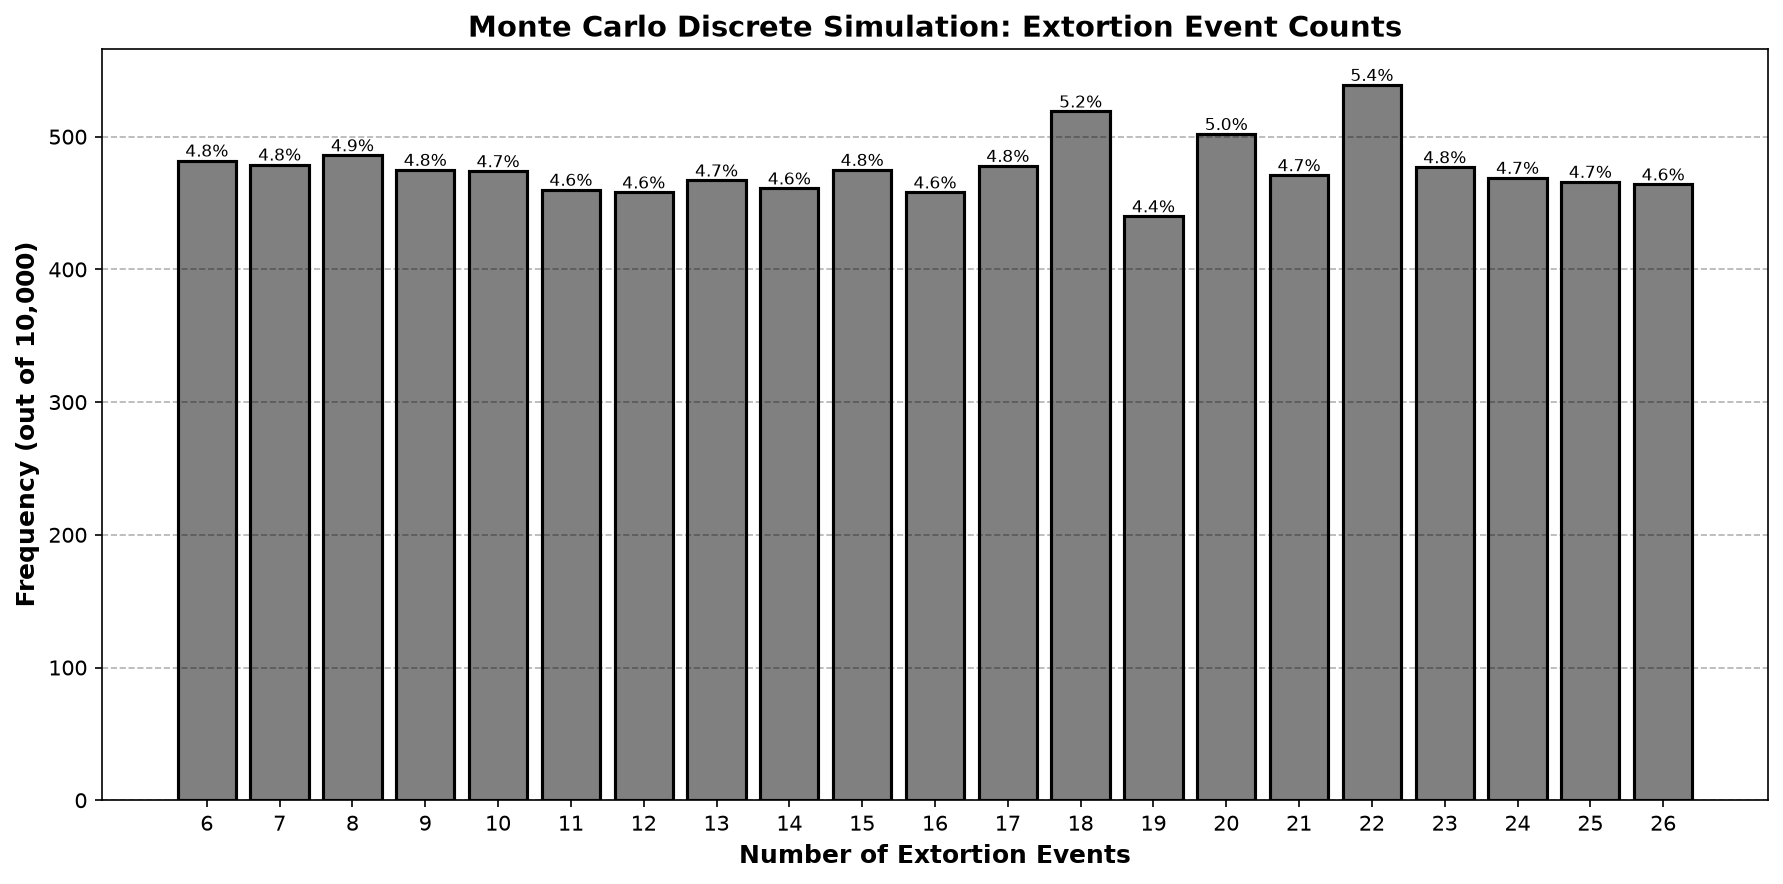
\includegraphics[width=\linewidth]{figures/discrete_extortion_count.png}}}
  \caption{We ran a\index{Monte Carlo simulation} Monte Carlo simulation of 10,000 iterations with a discrete distribution to spread random instances between upper and lower bounds taken from the means of seven year samples. We bounded between 6 and 26 possible \index{extortion}extortion events over a year.\protect\endnote{\index{sample} Sample size was set equivalent to the City of\index{Chattanooga} Chattanooga to determine the per capita rates for each year over data from \index{American Samoa} American Samoa and\index{California} California.  The means of those rates were used to set upper and lower bounds with \index{American Samoa} American Samoa and\index{California} California representing low and high \index{cybercrime} cybercrime counts respectively.}
  \protect\endnote{Monte Carlo Modeling Toolkit authored by Derek E. Brink, CISSP, \url{www.linkedin.com/in/derekbrink}. March 2023.}
  }
  \label{fig:screenshot-montecarlo-extortion-count-discrete}
\end{figure}
When we computed the upper and lower bounds, we recognized that a normal distribution would not fit well for forecasting likelihood.  We took the mean of the sample from American Samoa for the lower bound (5.60, rounded to 6); we took the mean from the sample from California for the upper bound (26.48, rounded to 26); we had a separation of 20 units.  Therefore, we switched to a discrete model with all 21 options sharing an equal likelihood.
\begin{table}[H]
  \centering
  \caption{Monte Carlo Discrete Simulation Values for Extortion}
  \label{tab:discrete_extortion_montecarlo}
  \begin{center}
  \begin{tabular}{@{}>{\centering\arraybackslash}
  p{0.20\linewidth} >{\centering\arraybackslash}
  p{0.10\linewidth} >{\centering\arraybackslash}
  p{0.10\linewidth} >{\centering\arraybackslash}
  p{0.10\linewidth} >{\centering\arraybackslash}
  p{0.10\linewidth} >{\centering\arraybackslash}
  p{0.10\linewidth}}
    \toprule
Events
    &6
    &7
    &8
    &9
    &10\\
    \midrule
Likelihood
    &4.8\%
    &4.8\%
    &4.8\%
    &4.8\%
    &4.8\%\\
    \bottomrule \end{tabular}
  \begin{tabular}{@{}>{\centering\arraybackslash}
  p{0.20\linewidth} >{\centering\arraybackslash}
  p{0.10\linewidth} >{\centering\arraybackslash}
  p{0.10\linewidth} >{\centering\arraybackslash}
  p{0.10\linewidth} >{\centering\arraybackslash}
  p{0.10\linewidth} >{\centering\arraybackslash}
  p{0.10\linewidth}}
    \toprule
Events
    &11
    &12
    &13
    &14
    &15\\
    \midrule
Likelihood
    &4.8\%
    &4.8\%
    &4.8\%
    &4.8\%
    &4.8\%\\
    \bottomrule \end{tabular}
  \begin{tabular}{@{}>{\centering\arraybackslash}
  p{0.20\linewidth} >{\centering\arraybackslash}
  p{0.10\linewidth} >{\centering\arraybackslash}
  p{0.10\linewidth} >{\centering\arraybackslash}
  p{0.10\linewidth} >{\centering\arraybackslash}
  p{0.10\linewidth} >{\centering\arraybackslash}
  p{0.10\linewidth}}
    \toprule
Events
    &16
    &17
    &18
    &19
    &20\\
    \midrule
Likelihood
    &4.8\%
    &4.8\%
    &4.8\%
    &4.8\%
    &4.8\%\\
    \bottomrule \end{tabular}
  \begin{tabular}{@{}>{\centering\arraybackslash}
  p{0.20\linewidth} >{\centering\arraybackslash}
  p{0.10\linewidth} >{\centering\arraybackslash}
  p{0.10\linewidth} >{\centering\arraybackslash}
  p{0.10\linewidth} >{\centering\arraybackslash}
  p{0.10\linewidth} >{\centering\arraybackslash}
  p{0.10\linewidth}}
    \toprule
Events
    &21
    &22
    &23
    &24
    &25\\
    \midrule
Likelihood
    &4.8\%
    &4.8\%
    &4.8\%
    &4.8\%
    &4.8\%\\
    \bottomrule \end{tabular}
  \begin{tabular}{@{}>{\centering\arraybackslash}
  p{0.20\linewidth} >{\centering\arraybackslash}
  p{0.10\linewidth}}
    \toprule
Events
    &26\\
    \midrule
Likelihood
    &4.8\%\\
    \bottomrule \end{tabular}
    \end{center}
  \raggedright{A\index{Monte Carlo simulation} Monte Carlo simulation was run using a discrete distribution.  We bounded the simulation between 6 and 26 events.  We assigned an approximately 4.8\% likelihood to each bin.  The resulting distribution showed the effect of randomness on each possible outcome.}
\end{table}

%%%%%%%%%%%%%%%%%%%%  IPR %%%%%%%%%%%%%%%%%%%%%%%%
\newpage
\subsection{Intellectual Property Rights (\gls{ipr})}\label{sec:ipr}
\subsubsection{Lower Bound Computation}
\[
\begin{bmatrix}
\mathbf{x}_{\text{American Samoa}}^{(\text{count})}\\
\mathbf{x}_{\text{American Samoa}}^{(\text{dollars})}
\end{bmatrix}
=
\begin{bmatrix}
0 & \cdots & 0 & \cdots & 0\\
\$0 & \cdots & \$0 & \cdots & \$0
\end{bmatrix}.
\]
% Columns represent years 2016, \cdots, 2017, \cdots, 2022 for American Samoa IPR/Counterfeit.
% Raw counts: 2016=0, 2017=0, 2022=0.  Raw dollars: 2016=\$0, 2017=\$0, 2022=\$0.
\[
\begin{bmatrix}
\mathbf{x}_{\text{American Samoa}}^{(\text{count scaled to sample population})}\\
\mathbf{x}_{\text{American Samoa}}^{(\text{dollars scaled to sample population})}
\end{bmatrix}
=
\begin{bmatrix}
0 & \cdots & 0 & \cdots & 0\\
\$0 & \cdots & \$0 & \cdots & \$0
\end{bmatrix}.
\]
% Per-capita scaled to Chattanooga population: 2016=0, 2017=0, 2022=0 victims; dollars: all \$0.
\[
\bar{X}_{\text{American Samoa}}^{(m)}
= \frac{1}{N}\sum_{i=1}^{N} X_{\text{American Samoa},i}^{(m)},
\]
\\
\[
\qquad
m \in \{\text{scaled count},\text{scaled dollars}\}
\]
\[
\begin{bmatrix}
\bar{X}_{\text{American Samoa}}^{(\text{scaled count})}\\
\bar{X}_{\text{American Samoa}}^{(\text{scaled dollars})}
\end{bmatrix}
=
\begin{bmatrix}
0.43\\
\$0
\end{bmatrix}.
\]
% Mean of 7-year scaled counts (0,0,0,0,0,3,0) = 3/7 = 0.43.  All dollar values = \$0.
\subsubsection{Upper Bound Computation}
\[
\begin{bmatrix}
\mathbf{x}_{\text{California}}^{(\text{count})}\\
\mathbf{x}_{\text{California}}^{(\text{dollars})}
\end{bmatrix}
=
\begin{bmatrix}
383 & \cdots & 399 & \cdots & 318\\
\$1{,}946{,}413 & \cdots & \$1{,}750{,}437 & \cdots & \$1
\end{bmatrix}.
\]
% Columns represent years 2016, \cdots, 2017, \cdots, 2022 for California IPR/Counterfeit.
% Raw counts: 2016=383, 2017=399, 2022=318.
% Raw state losses: 2016=\$1,946,413; 2017=\$1,750,437; 2022=\$1 (data anomaly in source report).
\[
\begin{bmatrix}
\mathbf{x}_{\text{California}}^{(\text{count scaled to sample population})}\\
\mathbf{x}_{\text{California}}^{(\text{dollars scaled to sample population})}
\end{bmatrix}
=
\begin{bmatrix}
1 & \cdots & 1 & \cdots & 1\\
\$5{,}082 & \cdots & \$4{,}387 & \cdots & \$734
\end{bmatrix}.
\]
% Per-capita scaled to Chattanooga population:
% 2016=1 victim, \$5,082; 2017=1 victim, \$4,387; 2022=1 victim, \$734.
\[
\bar{X}_{\text{California}}^{(m)}
= \frac{1}{N}\sum_{i=1}^{N} X_{\text{California},i}^{(m)},
\]
\\
\[
\qquad
m \in \{\text{scaled count},\text{scaled dollars}\}
\]
\[
\begin{bmatrix}
\bar{X}_{\text{California}}^{(\text{scaled count})}\\
\bar{X}_{\text{California}}^{(\text{scaled dollars})}
\end{bmatrix}
=
\begin{bmatrix}
1.29\\
\$5{,}199
\end{bmatrix}.
\]
% Mean of 7-year scaled counts (1,1,1,1,2,2,1) = 9/7 = 1.29.
% Mean of 7-year scaled losses (\$5082+\$4387+\$4879+\$9228+\$6663+\$5422+\$734)/7 = \$5,199.
\subsubsection{Monte Carlo Simulations for Likelihood and Impact}
\begin{figure}[H]
  \centering
  \rotatebox{0}{\scalebox{1}{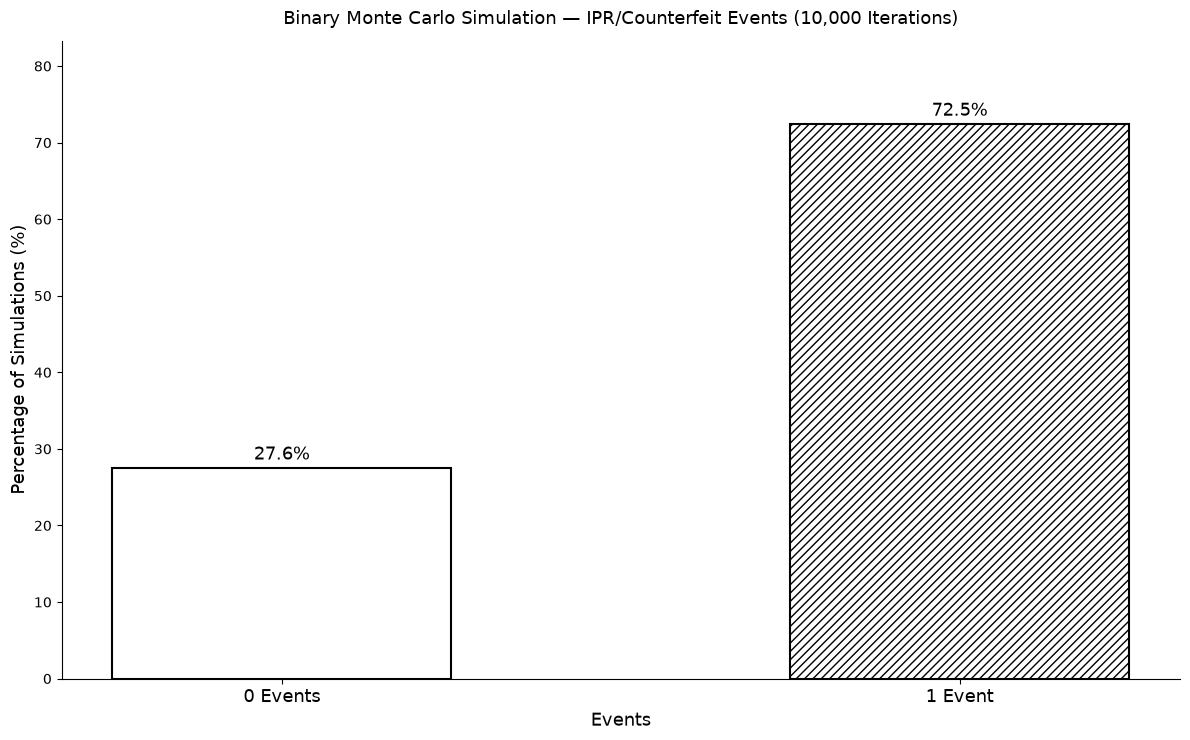
\includegraphics[width=\linewidth]{figures/binary_ipr_count.png}}}
  \caption{We ran a\index{Monte Carlo simulation} Monte Carlo simulation of 10,000 iterations with a \gls{binary} distribution to
  spread random instances between upper and lower bounds taken from the means of seven year samples.
  We bounded between 0 and 1 possible \index{intellectual property rights} intellectual property rights
  (\gls{ipr}) events over a year.\protect\endnote{\index{sample} Sample size was set equivalent to the
  City of\index{Chattanooga} Chattanooga to determine the per capita rates for each year over data
  from \index{American Samoa} American Samoa and\index{California} California.  The means of those
  rates were used to set upper and lower bounds with \index{American Samoa} American Samoa
  and\index{California} California representing low and high \index{cybercrime} \gls{cybercrime} counts
  respectively.}
  \protect\endnote{Monte Carlo Modeling Toolkit authored by Derek E.\ Brink, \gls{cissp},
  \url{www.linkedin.com/in/derekbrink}. March 2023.}
  }
  \label{fig:screenshot-montecarlo-ipr-count-binary}
\end{figure}

When we computed the upper and lower bounds, we recognized that a normal distribution would not fit
well for forecasting likelihood.  We took the mean of the sample from American Samoa for the lower
bound (0.43); we took the mean from the sample from California for the upper bound (1.29); we had a
separation of 0.86 units.  Because the confidence bounds are between 0 and 1, we used a \gls{binary} model.
A \gls{binary} distribution assigns a probability to 0 or 1 events occurring.  We set the probability of
one \gls{ipr}/Counterfeit event at approximately 71.4\%---the midpoint between the lower bound probability
(0.43) and the upper bound probability (capped at 1.0).

\begin{table}[H]
  \centering
  \caption{Monte Carlo \gls{binary} Simulation Values for Intellectual Property Rights (\gls{ipr})}
  \label{tab:binary_ipr_montecarlo}
  \begin{center}
  \begin{tabular}{@{}>{\centering\arraybackslash}
  p{0.30\linewidth} >{\centering\arraybackslash}
  p{0.15\linewidth} >{\centering\arraybackslash}
  p{0.15\linewidth}}
    \toprule
Events  & 0 & 1\\
    \midrule
Likelihood  & 27.6\% & 72.5\%\\
    \bottomrule
  \end{tabular}
  \end{center}
  \raggedright{A\index{Monte Carlo simulation} Monte Carlo simulation was run using a \gls{binary}
  distribution.  We bounded the simulation between 0 and 1 events.  We assigned approximately a
  71.4\% probability to one event occurring.  The resulting distribution showed the effect of
  randomness; the simulation produced 0 events 27.6\% of the time and 1 event 72.5\% of the time.}
\end{table}


%%%%%%%%%%%%%%%%%%%%  IDENTITY THEFT %%%%%%%%%%%%%%%%%%%%%%%%
\newpage
\subsection{Identity Theft}\label{sec:identitytheft}
\subsubsection{Lower Bound Computation}
\[
\begin{bmatrix}
\mathbf{x}_{\text{American Samoa}}^{(\text{count})}\\
\mathbf{x}_{\text{American Samoa}}^{(\text{dollars})}
\end{bmatrix}
=
\begin{bmatrix}
0 & \cdots & 0 & \cdots & 2\\
\$0 & \cdots & \$0 & \cdots & \$600
\end{bmatrix}.
\]
% Columns represent years 2016, \cdots, 2017, \cdots, 2022 for American Samoa Identity Theft.
% Raw counts: 2016=0, 2017=0, 2022=2.  Raw dollars: 2016=$0, 2017=$0, 2022=$600.
\[
\begin{bmatrix}
\mathbf{x}_{\text{American Samoa}}^{(\text{count scaled to sample population})}\\
\mathbf{x}_{\text{American Samoa}}^{(\text{dollars scaled to sample population})}
\end{bmatrix}
=
\begin{bmatrix}
0 & \cdots & 0 & \cdots & 8\\
\$0 & \cdots & \$0 & \cdots & \$2{,}100
\end{bmatrix}.
\]
% Per-capita scaled to Chattanooga population: 2016=0, 2017=0, 2022=8 victims; dollars: 2016=$0, 2017=$0, 2022=$2,100.
  \[
\bar{X}_{\text{American Samoa}}^{(m)}
= \frac{1}{N}\sum_{i=1}^{N} X_{\text{American Samoa},i}^{(m)},
\]
\\
\[
\qquad
m \in \{\text{scaled count},\text{scaled dollars}\}
\]
\[
\begin{bmatrix}
\bar{X}_{\text{American Samoa}}^{(\text{scaled count})}\\
\bar{X}_{\text{American Samoa}}^{(\text{scaled dollars})}
\end{bmatrix}
=
\begin{bmatrix}
2\\
\$300
\end{bmatrix}.
\]
\subsubsection{Upper Bound Computation}
\[
\begin{bmatrix}
\mathbf{x}_{\text{California}}^{(\text{count})}\\
\mathbf{x}_{\text{California}}^{(\text{dollars})}
\end{bmatrix}
=
\begin{bmatrix}
2{,}368 & \cdots & 2{,}609 & \cdots & 2{,}854\\
\$17{,}862{,}807 & \cdots & \$10{,}216{,}795 & \cdots & \$27{,}903{,}539
\end{bmatrix}.
\]
% Columns represent years 2016, \cdots, 2017, \cdots, 2022 for California Identity Theft.
\[
\begin{bmatrix}
\mathbf{x}_{\text{California}}^{(\text{count scaled to sample population})}\\
\mathbf{x}_{\text{California}}^{(\text{dollars scaled to sample population})}
\end{bmatrix}
=
\begin{bmatrix}
10 & \cdots & 11 & \cdots & 13\\
\$75{,}434 & \cdots & \$43{,}076 & \cdots & \$127{,}101
\end{bmatrix}.
\]
\[
\bar{X}_{\text{California}}^{(m)}
= \frac{1}{N}\sum_{i=1}^{N} X_{\text{California},i}^{(m)},
\]
\\
\[
\qquad
m \in \{\text{scaled count},\text{scaled dollars}\}
\]
\[
\begin{bmatrix}
\bar{X}_{\text{California}}^{(\text{scaled count})}\\
\bar{X}_{\text{California}}^{(\text{scaled dollars})}
\end{bmatrix}
=
\begin{bmatrix}
12\\
\$118{,}823
\end{bmatrix}.
\]
\subsubsection{Monte Carlo Simulations for Likelihood and Impact}
\begin{figure}[H]
  \centering
  \rotatebox{0}{\scalebox{1}{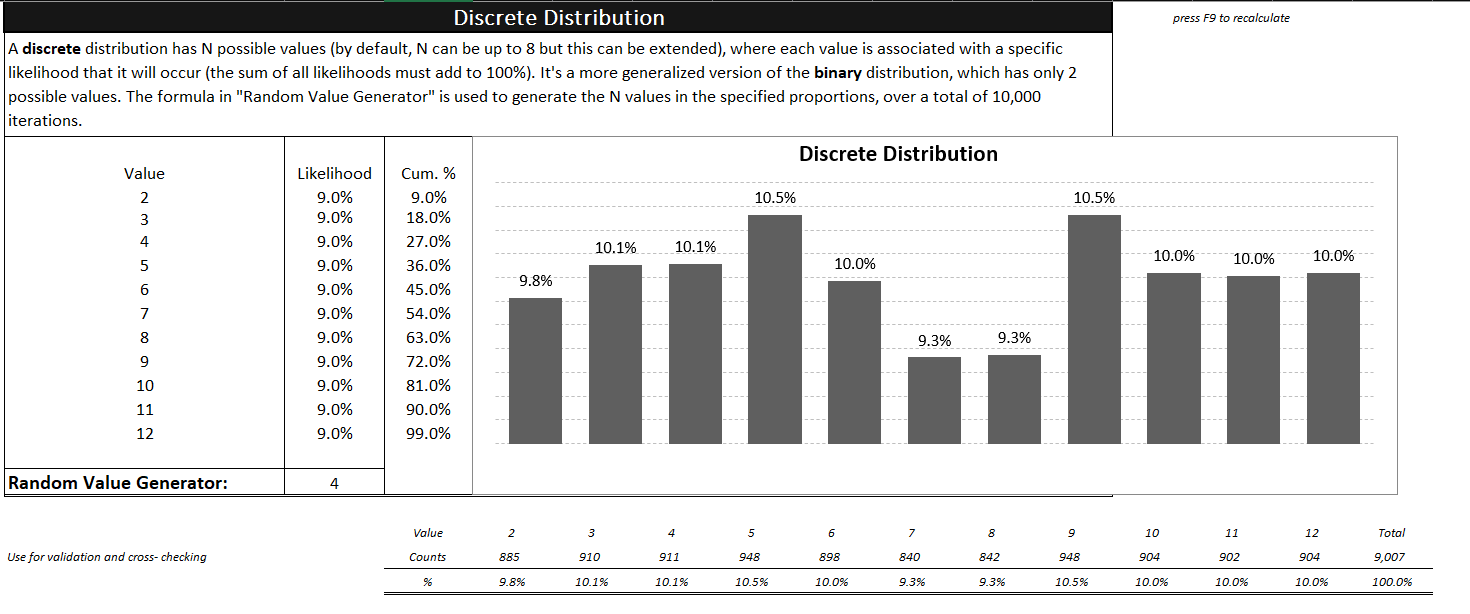
\includegraphics[width=\linewidth]{figures/discrete_idtheft_count.png}}}
  \caption{We ran a\index{Monte Carlo simulation} Monte Carlo simulation of 10,000 iterations with a discrete distribution to spread random instances between confidence intervals taken from the means of seven year samples. We bounded between 2 and 12 possible \index{identity theft}identity theft events over a year.\protect\endnote{\index{sample} Sample size was set equivalent to the City of\index{Chattanooga} Chattanooga to determine the per capita rates for each year over data from \index{American Samoa} American Samoa and\index{California} California.  The means of those rates were used to set 10\% and 90\%\index{confidence interval} confidence intervals with \index{American Samoa} American Samoa and\index{California} California representing low and high \index{cybercrime} cybercrime counts respectively.}
  \protect\endnote{Monte Carlo Modeling Toolkit authored by Derek E. Brink, \gls{cissp}, \url{www.linkedin.com/in/derekbrink}. March 2023.}
  }
  \label{fig:screenshot-montecarlo-idtheft-count-discrete}
\end{figure}
When we computed the upper and lower bounds, we recognized that a normal distribution would not fit well for forecasting likelihood.  We took the mean of the sample from American Samoa for the lower bound (2); we took the mean from the sample from California for the upper bound (12); we had a separation of 10 units.  Therefore, we switched to a discrete model with all 11 options sharing an equal likelihood.
\begin{table}[H]
  \centering
  \caption{Monte Carlo Discrete Simulation Values for Identity Theft}
  \label{tab:discrete_idtheft_montecarlo}
  \begin{center}
  \begin{tabular}{@{}>{\centering\arraybackslash}
  p{0.20\linewidth} >{\centering\arraybackslash}
  p{0.10\linewidth} >{\centering\arraybackslash}
  p{0.10\linewidth} >{\centering\arraybackslash}
  p{0.10\linewidth} >{\centering\arraybackslash}
  p{0.10\linewidth} >{\centering\arraybackslash}
  p{0.10\linewidth} >{\centering\arraybackslash}
  p{0.10\linewidth}}
    \toprule
Events
&2
&3
&4
&5
&6
&7\\
    \midrule
Likelihood    
&8.9\%
&9.5\%
&9.1\%
&8.8\%
&9.4\%
&9.7\%\\
    \bottomrule \end{tabular}
\begin{tabular}{@{}>{\centering\arraybackslash}
  p{0.20\linewidth} >{\centering\arraybackslash}
  p{0.10\linewidth} >{\centering\arraybackslash}
  p{0.10\linewidth} >{\centering\arraybackslash}
  p{0.10\linewidth} >{\centering\arraybackslash}
  p{0.10\linewidth} >{\centering\arraybackslash}
  p{0.10\linewidth}}
    \toprule
Events    
    &8
    &9
    &10
    &11
    &12\\
    \midrule
Likelihood
&9.1\%
&9.4\%
&8.6\%
&8.3\%
&9.2\%\\
    \bottomrule \end{tabular}
    \end{center}
  \raggedright{A\index{Monte Carlo simulation} Monte Carlo simulation was run using a discrete distribution.  We bounded the simulation between 2 and 12 events.  We assigned a $\approx$9.1\% likelihood to each bin.  The resulting distribution showed the effect of randomness on each possible outcome.}
\end{table}

%%%%%%%%%%%%%%  BUSINESS EMAIL COMPROMISE %%%%%%%%%%%%%%%%%%%%
\newpage
\subsection{Business Email Compromise}\label{sec:bec}
\subsubsection{Lower Bound Computation}
\[
\begin{bmatrix}
\mathbf{x}_{\text{American Samoa}}^{(\text{count})}\\
\mathbf{x}_{\text{American Samoa}}^{(\text{dollars})}
\end{bmatrix}
=
\begin{bmatrix}
0 & 0 & \cdots & 2\\
\$0 &\$0 & \cdots &\$960 
\end{bmatrix}.
\]
\[
\begin{bmatrix}
\mathbf{x}_{\text{American Samoa}}^{(\text{count scaled to sample population})}\\
\mathbf{x}_{\text{American Samoa}}^{(\text{dollars scaled to sample population})}
\end{bmatrix}
=
\begin{bmatrix}
0 & 0 & \cdots & 8\\
\$0 & \$0 & \cdots &\$3{,}360
\end{bmatrix}.
\]
  \[
\bar{X}_{\text{American Samoa}}^{(m)}
= \frac{1}{N}\sum_{i=1}^{N} X_{\text{American Samoa},i}^{(m)},
\]
\\
\[
\qquad
m \in \{\text{scaled count},\text{scaled dollars}\}
\]
\[
\begin{bmatrix}
\bar{X}_{\text{American Samoa}}^{(\text{scaled count})}\\
\bar{X}_{\text{American Samoa}}^{(\text{scaled dollars})}
\end{bmatrix}
=
\begin{bmatrix}
4\\
\$13{,}851
\end{bmatrix}.
\]
\subsubsection{Upper Bound Computation}
\[
\begin{bmatrix}
\mathbf{x}_{\text{California}}^{(\text{count})}\\
\mathbf{x}_{\text{California}}^{(\text{dollars})}
\end{bmatrix}
=
\begin{bmatrix}
2{,}155 & 2{,}429 & \cdots & 3{,}269\\
\$69{,}208{,}381 &\$106{,}225{,}791  & \cdots &\$439{,}425{,}357 
\end{bmatrix}.
\]
\[
\begin{bmatrix}
\mathbf{x}_{\text{California}}^{(\text{count scaled to sample population})}\\
\mathbf{x}_{\text{California}}^{(\text{dollars scaled to sample population})}
\end{bmatrix}
=
\begin{bmatrix}
9 & 11 & \cdots & 15\\
\$289{,}037 &\$481{,}055 & \cdots &\$2{,}016{,}329 
\end{bmatrix}.
\]
\[
\bar{X}_{\text{California}}^{(m)}
= \frac{1}{N}\sum_{i=1}^{N} X_{\text{California},i}^{(m)},
\]
\\
\[
\qquad
m \in \{\text{scaled count},\text{scaled dollars}\}
\]
\[
\begin{bmatrix}
\bar{X}_{\text{California}}^{(\text{scaled count})}\\
\bar{X}_{\text{California}}^{(\text{scaled dollars})}
\end{bmatrix}
=
\begin{bmatrix}
13\\
\$784{,}561
\end{bmatrix}.
\]
\subsubsection{Monte Carlo Simulations for Likelihood and Impact}
\begin{figure}[H]
  \centering
  \rotatebox{0}{\scalebox{1}{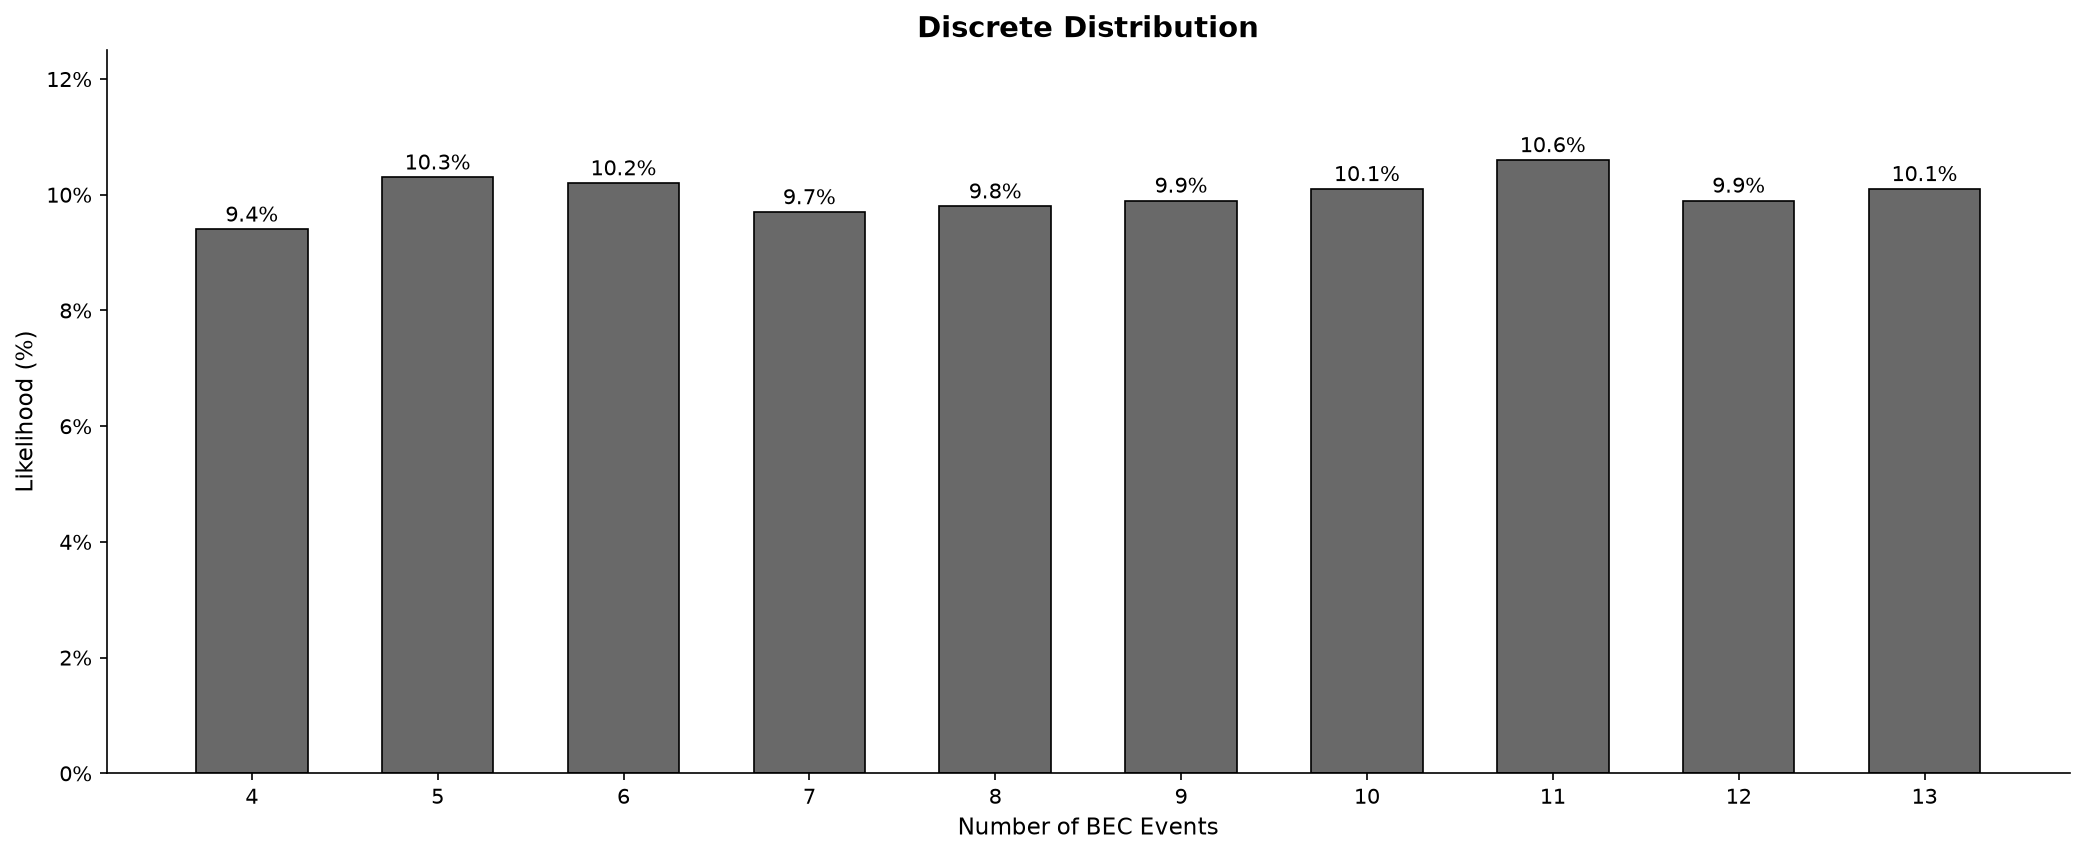
\includegraphics[width=\linewidth]{figures/discrete_bec_count.png}}}
  \caption{We ran a\index{Monte Carlo simulation} Monte Carlo simulation of 10,000 iterations with a discrete distribution to spread random instances between confidence intervals taken from the means of seven year samples. We bounded between 4 and 13 possible \index{business email compromise}business email compromise events over a year.\protect\endnote{\index{sample} Sample size was set equivalent to the City of\index{Chattanooga} Chattanooga to determine the per capita rates for each year over data from \index{American Samoa} American Samoa and\index{California} California.  The means of those rates were used to set lower and upper bounds with \index{American Samoa} American Samoa and\index{California} California representing low and high \index{cybercrime} \gls{cybercrime} counts respectively.}
  \protect\endnote{Monte Carlo Modeling Toolkit authored by Derek E. Brink, \gls{cissp}, \url{www.linkedin.com/in/derekbrink}. March 2023.}
  }
  \label{fig:screenshot-montecarlo-bec-count-discrete}
\end{figure}
When we computed the upper and lower bounds, we recognized that a normal distribution would not fit well for forecasting likelihood.  We took the mean of the sample from American Samoa for the lower bound (4); we took the mean from the sample from California for the upper bound (13); we had a separation of 9 units.  Therefore, we switched to a discrete model with all 10 options sharing an equal likelihood.
\begin{table}[H]
  \centering
  \caption{Monte Carlo Discrete Simulation Values for Business Email Compromise}
  \label{tab:discrete_bec_montecarlo}
  \begin{center}
  \begin{tabular}{@{}>{\centering\arraybackslash}
  p{0.20\linewidth} >{\centering\arraybackslash}
  p{0.10\linewidth} >{\centering\arraybackslash}
  p{0.10\linewidth} >{\centering\arraybackslash}
  p{0.10\linewidth} >{\centering\arraybackslash}
  p{0.10\linewidth} >{\centering\arraybackslash}
  p{0.10\linewidth}}
    \toprule
Events
&4
&5
&6
&7
&8\\
    \midrule
Likelihood    
&9.4\%
&10.3\%
&10.2\%
&9.7\%
&9.8\%\\
    \bottomrule \end{tabular}
\begin{tabular}{@{}>{\centering\arraybackslash}
  p{0.20\linewidth} >{\centering\arraybackslash}
  p{0.10\linewidth} >{\centering\arraybackslash}
  p{0.10\linewidth} >{\centering\arraybackslash}
  p{0.10\linewidth} >{\centering\arraybackslash}
  p{0.10\linewidth} >{\centering\arraybackslash}
  p{0.10\linewidth}}
    \toprule
Events    
    &9
    &10
    &11
    &12
    &13\\
    \midrule
Likelihood
&9.9\%
&10.1\%
&10.6\%
&9.9\%
&10.1\%\\
    \bottomrule \end{tabular}
    \end{center}
  \raggedright{A\index{Monte Carlo simulation} Monte Carlo simulation was run using a discrete distribution.  We bounded the simulation between 4 and 13 events.  We assigned a 10\% likelihood to each bin.  The resulting distribution showed the effect of randomness on each possible outcome.}
\end{table}

\section{Discussion}

\subsection{Why Some Categories Might Be Lower}
As we look over some of our generated statistics, we can see that sometimes our expectations were defied.  Why, for example, are some of the categories so low in likelihood?  At our level of access to the data from \gls{ic3}, we don't know more of the background details that might point directly to a cause for that.  Perhaps law enforcement gets better insight; but, we have to make do with what we have.  Let's consider some of the categories and suppose, arbitrarily and based on our experience, why some of the figures might be the way they are.

First, we have the overall effect of the convenience sample.  As we mentioned earlier, these reports are based on voluntary disclosures to \gls{us} \gls{fbi} \gls{ic3}.  That means that we could see lower numbers in areas where victims were not motivated to disclose.

Potential victims could also have successful mitigation efforts in place.  For example, we see lower corporate data breaches than personal data breaches.  Persumably, corporations have security departments that can help them to operate enterprise grade defensive tools when individual people cannot.  Also, we see low counts in \gls{malware} and \gls{ransomware} when those categories are often in the news.  It could be that conventional antivirus scanners and endpoint defenses do a good job of neutralizing known \gls{malware} threats.  If a large number of antivirus users are being protected successfully, then we might have a small number of victimization claims to the \gls{ic3}.


\subsection{Crimes Against Children and Complaints}

\subsection{Business Email Compromise Versus \gls{ransomware}}
A long standing pattern of expectation is that a user will be phished, \gls{malware} will be deployed on their machine, and then a company will face a \gls{ransomware} \gls{attack}.  Besides this, we see a business email compromise category.  If \gls{bec} is a precedent \gls{attack}, then why aren't its numbers higher?

One of the reasons could be the ramifications of the attacks and their flow into later reporting classifications.  \gls{bec}
attacks could also flow in other directions like credential stuffing attacks or passive surveillance. In credential stuffing, the known business email address might be reused in later follow-on attacks to other systems.  If an attacker chooses a victim that's a key individual in the company, then passive surveillance of the email account might yield valuable information.  Several 10K reports cite top executives getting their accounts monitored through what looks like a combination of passive surviellance and \gls{bec}.

These hint in the numbers can suggest to us an illustration that the overall classification of an \gls{attack} may not offer direct insight on all of the tactics and techniques that concern us as defenders.  This shouldn't surprise us; we see plenty of evidence in MITRE ATT\&CK, for instance, that most \gls{apt}s use several layers of \gls{ttps}.

\section{Summary of Cybercrime Analysis References}

Tables~\ref{tab:\gls{cybercrime}-anova-summary-1} and~\ref{tab:cybercrime\index{cybercrime}-anova-summary-2} provide a comprehensive reference guide for the quantitative analysis conducted on each \gls{cybercrime} category in this chapter. These tables summarize the locations of lower bound computations, upper bound computations, Monte Carlo simulation figures, and simulation value tables that can be used for risk assessment after ANOVA validation.


\begin{table}[htbp]
\centering
\caption{Alignment of Retained Cybercrime Categories with MITRE ATT\&CK Techniques: Categories and Tactics}
\label{tab:attack_alignment_1}
\begin{tabular}{|p{3.5cm}|p{4.5cm}|}
\hline
\textbf{Category} & \textbf{ATT\&CK Tactic} \\
\hline
Personal Data Breach & Collection, Exfiltration \\
\hline
Phishing & Initial Access \\
\hline
Ransomware & Impact \\
\hline
Extortion & Impact \\
\hline
IPR / Counterfeit & Collection, Exfiltration \\
\hline
Identity Theft & Credential Access \\
\hline
BEC & Initial Access, Credential Access, Impact \\
\hline
\end{tabular}
\end{table}

\begin{table}[htbp]
\centering
\caption{Alignment of Retained Cybercrime Categories with MITRE ATT\&CK Techniques: Representative Techniques}
\label{tab:attack_alignment_2}
\begin{tabular}{|p{3.5cm}|p{8.0cm}|}
\hline
\textbf{Category} & \textbf{Representative ATT\&CK Techniques} \\
\hline
Personal Data Breach & Data from Information Repositories (T1213), Archive Collected Data (T1560), Exfiltration Over Web Services (T1567) \\
\hline
Phishing & \gls{phishing} (T1566), Phishing Attachment (T1566.001), Phishing Link (T1566.002), Spearphishing (T1566) \\
\hline
Ransomware & Data \gls{encrypt}ed for Impact (T1486), Financial Theft (T1657) \\
\hline
Extortion & Financial Theft (T1657), Data Encrypted for Impact (T1486), Data Leak Threats associated with double-extortion campaigns \\
\hline
IPR / Counterfeit & Data from Information Repositories (T1213), Exfiltration Over Web Services (T1567), Automated Collection (T1119) \\
\hline
Identity Theft & Credentials from \gls{password} Stores (T1555), Steal or Forge \gls{authentication} Credentials (T1649), Brute Force (T1110) \\
\hline
BEC & Phishing (T1566), Valid Accounts (T1078), Financial Theft (T1657), Account Manipulation (T1098) \\
\hline
\end{tabular}
\end{table}



\markchapterendnotes